\documentclass[12pt,twoside]{report}
\usepackage{titlesec}         %para 4 níveis de subsection com numeração
\setcounter{secnumdepth}{4}   %para 4 níveis de subsection com numeração
\setcounter{tocdepth}{4}      %pata 4 níveis no TOC com numeração aparecendo
%\documentclass[12pt,a4paper]{ltxdoc}
%\documentclass[12pt,a4paper]{article}
\usepackage{lmodern}			% Usa a fonte Latin Modern			
\usepackage[T1]{fontenc}		% seleção de códigos de fonte.
\usepackage[utf8]{inputenc}		% determina a codificação utilizada (conversão automática dos acentos)
\usepackage[breaklinks]{hyperref}
\usepackage{parskip}			% espaçamento entre os parágrafos
\usepackage{microtype} 			% para melhorias de justificação
\usepackage{morefloats}			% permite mais floats
\usepackage{setspace}
%\singlespacing
\onehalfspacing
%\doublespacing
%\setstretch{1.1}

%\documentclass[10pt,a4paper]{article}
\usepackage[utf8]{inputenc}
\usepackage[english]{babel}
\usepackage{amsmath}
\usepackage{amsfonts}
\usepackage{amssymb}
\usepackage{graphicx}
\usepackage{algorithm,algorithmic}
\usepackage{xcolor}
%Alessandro input: makecell package to permite line break inside tables
\usepackage{makecell}
\usepackage[alf]{abntex2cite}	% citacoes

%\documentclass[12pt,twoside]{report}
%\usepackage[utf8]{inputenc}
%\usepackage{graphicx}
\graphicspath{ {images/} }
%\usepackage{caption}
%\usepackage{subcaption}
\usepackage[a4paper,width=150mm,top=25mm,bottom=25mm,bindingoffset=6mm]{geometry}
\usepackage{fancyhdr}
\pagestyle{fancy}
%
\renewcommand{\headrulewidth}{0.4pt}
\renewcommand{\footrulewidth}{0.4pt}

%\usepackage[style=authoryear,sorting=none]{biblatex}
%\addbibresource{references.bib}

\title{Automated Verification of Stand-alone Solar Photovoltaic Systems: Optimal Sizing and Project Validation}
\author{Alessandro Trindade}
\date{31 July 2019}

\begin{document}

\begin{titlepage}
    \begin{center}
        \vspace*{1cm}
        
        \Huge
        \textbf{Automated Verification Applied to Stand-alone Solar Photovoltaic Systems}
        
        \vspace{0.5cm}
        \LARGE
        Optimal Sizing and Project Validation
        
        \vspace{1.5cm}
        
        \textbf{Alessandro Bezerra Trindade}
        
        \vfill
        
        A thesis presented for the degree of\\
        Doctor of Philosophy in Informatics
        
        \vspace{0.8cm}
        
        
\includegraphics[width=0.3\textwidth]{ufam_logo}
        
        \Large
        Computing Institute (IComp)\\
        Federal University of Amazonas (UFAM)\\
        Brazil\\
        July 2019
        
    \end{center}
\end{titlepage}

\begin{titlepage}
    \begin{center}
%        \vspace*{1cm}
        \Large
        Federal University of Amazonas (UFAM)\\
        Computing Institute (IComp)\\
		Graduate Program in Informatics (PPGI)\\

        \vspace*{1cm}
        
		\Large
		ALESSANDRO BEZERRA TRINDADE

        \vspace*{2cm}
        		        
        \Huge
        \textbf{Automated Verification of Stand-alone Solar Photovoltaic Systems}
        
        \vspace{0.5cm}
        \LARGE
        Optimal Sizing and Project Validation
        
        \vspace{2cm}
    \end{center}        
    
%        \vfill

\hspace{6cm}        A thesis submitted in partial fulfillment

\hspace{6cm}        of the requirements for the Degree of Doctor

\hspace{6cm}        of Philosophy in Informatics

\hspace{6cm}        Graduate Program in Informatics 

\hspace{6cm}        Federal University of Amazonas
        
        \vspace{2cm}
        
        \begin{center}
        Supervisor: Prof. Lucas Carvalho Cordeiro, Ph.D.\\
        \vspace{1cm}
        MANAUS\\
        2019\\
        \end{center}
\end{titlepage}
\thispagestyle{empty}
\pagenumbering{gobble}

\thispagestyle{plain}
%\begin{center}
%    \Large
%    \textbf{Automated Verification Applied to Stand-alone Solar Photovoltaic Systems}
%    
%    \vspace{0.4cm}
%    \large
%    Optimal Sizing and Project Validation
%    
%    \vspace{0.4cm}
%    \textbf{Alessandro Trindade}
%    
%    \vspace{0.9cm}
%    \textbf{Ficha Catalográfica elaborada por Suely O. Moraes - CRB 11/365}
%\end{center}
%
%
\thispagestyle{empty}
\null\vfill

\begin{center}
Ficha Catalográfica elaborada por Suely Oliveira Moraes – CRB 11/365
\begin{tabular}{|p{14.5cm}|}%{p{12cm}}
\hline
\begin{small}
\begin{verbatim}
       Trindade, Alessandro Bezerra.
T833a     Automated verification of stand-alone solar photovoltaic 
       systems: optimal sizing and project validation / Alessandro 
       Bezerra Trindade. Manaus: UFAM, 2020.

         130 fl.: il.: 21 cm 

         Orientador: Prof. PhD. Lucas Carvalho Cordeiro

         Tese (Doutorado em Informática) - Universidade Federal do
       Amazonas, Programa de Pós-Graduação em Informática. 

         1. Verificação formal. 2. Model checking. 3. Sistemas solares
       fotovoltaicos I. Cordeiro, Lucas Carvalho (Orient.) II. 
       Universidade Federal do Amazonas. III. Título.

                                               CDU 004.02:621.31(043.2)
\end{verbatim}
\end{small}
\\ \hline
\end{tabular}
\end{center}

\thispagestyle{plain}
%\thispagestyle{empty}
\newpage 

\thispagestyle{plain}
\begin{center}
%    \Large
%    \textbf{Automated Verification Applied to Stand-alone Solar Photovoltaic Systems}
%    
%    \vspace{0.4cm}
%    \large
%    Optimal Sizing and Project Validation
%    
%    \vspace{0.4cm}
%    \textbf{Alessandro Trindade}
%    
    \vspace{0.9cm}
    \textbf{Abstract}
\end{center}
With decreasing costs and increasing performance, the deployment of renewable energy systems is now growing faster now than in the past decade. In 2017, for the first time, the number of people without access to electricity dipped below 1 billion, but trends in energy access still fall short of global goals. Particular attention is given to stand-alone solar photovoltaic systems in rural areas or where grid extension is unfeasible. Tools to evaluate or to size electrification projects are available, but they are based on simulations that do not cover all aspects of the design space. However, the use of formal methods to model and validate any system has grown with time, mainly to find bugs in sophisticated hardware and software systems: they aim to establish system correctness with mathematical rigor. The use of formal methods in electrical systems is a new subject, with published research spanning only in the last four years.
Moreover, the use of automated synthesis in order to obtain the optimal sizing of solar photovoltaic systems has never been done before. This thesis marks the achievement of two major goals: first, the application of software model checking to verify formally the design of a stand-alone solar photovoltaic system, including solar panel, charge controller, battery, inverter, and electric load; second, a sound and automated approach to obtaining optimal sizing of stand-alone photovoltaic systems using program synthesis. For the  formal verification, we used case studies from real photovoltaic systems deployed in five different sites, ranging from 700 W to 1,200 W, in order to evaluate the proposed approach and to compare it with a specialized simulation tool. Different verification tools are evaluated also, in order to compare performance and soundness. Data from practical applications show the effectiveness of our proposed approach, where specific conditions that lead to failures in a photovoltaic solar system are detailed only by the automated verification method.
In addition, for the use of program synthesis, we propose a variant of the counterexample guided inductive synthesis (CEGIS) approach. This variant has two phases linking the technical and the cost analysis. First, we synthesize a feasible candidate based on power reliability, but which may not attain the lowest cost. Second, the candidate is then verified iteratively with a lower bound cost via symbolic model checking. If the verification step succeeds, the lower bound is adjusted; if it fails, a counterexample provides the optimal solution. The proposed synthesis method is novel and unprecedented as it streamlines the design of photovoltaic systems. Experimental results using seven case studies demonstrate that our synthesis method can produce optimal system sizing within an acceptable run-time. We also present a comparison with a specialized simulation tool over real photovoltaic systems in order to show the effectiveness of our approach, which can provide a more detailed and accurate solution than the simulation tool.

\textit{Keywords}: Formal verification; automated verification; model checking; program synthesis; electrical systems; and solar photovoltaic systems.

\pagestyle{empty}
%\thispagestyle{empty}
\newpage

\thispagestyle{plain}
\begin{center}
%    \Large
%    \textbf{Automated Verification Applied to Stand-alone Solar Photovoltaic Systems}
%    
%    \vspace{0.4cm}
%    \large
%    Optimal Sizing and Project Validation
%    
%    \vspace{0.4cm}
%    \textbf{Alessandro Trindade}
%    
    \vspace{0.9cm}
    \textbf{Resumo}
\end{center}
Com custos decrescentes e com melhoria de desempenho, a implantação de sistemas de energia renovável está crescendo cada vez mais rapidamente no mundo. Em 2017, pela primeira vez, o número de pessoas sem acesso a eletricidade ficou abaixo de 1 bilhão, mas os dados quanto à universalização do acesso a energia ficaram aquém das metas globais. Particular atenção é dada aos sistemas isolados solares fotovoltaicos em áreas rurais ou onde a extensão da rede é inviável. 
Ferramentas para avaliar ou dimensionar projetos de eletrificação estão disponíveis, mas elas são baseadas em simulações que não cobrem todos os aspectos do espaço de projeto. Por outro lado, o uso de métodos formais para modelar e validar qualquer tipo de sistema está crescendo com o tempo, principalmente para encontrar bugs em sistemas complexos de \textit{hardware} e \textit{software}: seu objetivo é estabelecer a corretude do sistema com rigor matemático. 
O uso de métodos formais em sistemas elétricos é um assunto recente, com pesquisas sendo publicadas apenas nos últimos quatro anos. Além disso, a síntese automatizada nunca foi usada antes para obter um ótimo dimensionamento de sistemas solares fotovoltaicos nunca foi feito antes. 
Esta tese marca duas conquistas principais: (1) a primeira aplicação de verificação de modelos de software para verificar o projeto de um sistema isolado solar fotovoltaico, incluindo painel solar, controlador de carga, bateria, inversor e carga elétrica; e (2) uma abordagem confiável e automatizada para obter o dimensionamento ótimo de sistemas fotovoltaicos usando a síntese de programas onde cada componente e função de um sistema solar fotovoltaico é descrito, incluindo suas propriedades, e o modelo comportamental que representa o dimensionamento ótimo é sintetizado automaticamente. 
Relacionado à verificação formal, estudos de caso de sistemas fotovoltaicos reais instalados em cinco localidades diferentes são usados para avaliar a abordagem proposta e para compará-la com ferramenta de simulação especializada.
Diferentes ferramentas de verificação são avaliadas também, a fim de comparar o desempenho e a confiabilidade dos resultados. Dados de aplicações práticas mostram a eficácia da abordagem proposta, onde condições específicas que levam a falhas em um sistema solar fotovoltaico são detalhadas apenas pelo método de verificação automatizado. 
Além disso, em relação ao uso da síntese de programas, propõe-se uma variante do método de síntese indutiva guiada por contraexemplos (CEGIS), com duas fases bem definidas: primeiro, ele sintetiza o dimensionamento de sistemas fotovoltaicos baseados em confiabilidade de energia, mas que pode não alcançar o menor custo; segundo, a solução proposta é então verificada iterativamente com um limite inferior via verificação de modelo simbólico. Se a etapa de verificação não falhar, o limite inferior será ajustado; e se falhar, o contraexemplo é fornecido com o dimensionamento ótimo, vinculando assim a resposta técnica da primeira fase à análise de custo da segunda fase. Os dados de equipamentos comerciais de diferentes fabricantes são fornecidos ao mecanismo de síntese e as soluções candidatas são derivadas da análise financeira do dimensionamento obtido. O método de síntese proposto é novo e sem precedentes para simplificar o projeto de sistemas fotovoltaicos. Resultados experimentais usando sete estudos de caso mostram que o nosso método de síntese é capaz de produzir em um tempo de execução aceitável o dimensionamento ótimo do sistema fotovoltaico, e um comparativo com uma ferramenta de simulação especializada e sistemas fotovoltaicos reais mostra a eficácia da abordagem adotada.



\textit{Palavras-chave}: Verificação formal; verificação automatizada; verificação de modelos; síntese de programa; sistemas elétricos; sistema solar fotovoltaico
%\thispagestyle{empty}

%\chapter*{Dedication}
%To mum and dad
%
%\chapter*{Declaration}
%I declare that..
%
\chapter*{Acknowledgements}
(It is not possible to get here without the help of several people. I hope I have not forgotten any and do no wrong).

I would like to thank God (for the gift of life); Solange and Louise (without the patience and support of my family I could not be here); my parents and grandparents; Lucas (for having believed in me and for the patience); the Electricity Department at UFAM (for the support); Professors Feitosa, Marco Cristo and Barreto from IComp (support and advice); IT support team from IComp (Virtual Machine maintenance); secretary people from IComp (for the administrative support); the financial support from FAPEAM, British Council/Newton Fund and Fundação Amazonas Sustentável; Davide Poggio from University of Sheffield for the HOMER Pro license (Research England QR GCRF Institutional Allocation); and Coventry University team (Elena, Kojo, and Ross for the opportunity to use field deployed photovoltaic solar systems).

\pagestyle{empty}

\tableofcontents

\listoffigures

\listoftables
\newpage 
\thispagestyle{plain}
\begin{center}
%    \Large
%    \textbf{Automated Verification Applied to Stand-alone Solar Photovoltaic Systems}
%    
%    \vspace{0.4cm}
%    \large
%    Optimal Sizing and Project Validation
%    
%    \vspace{0.4cm}
%    \textbf{Alessandro Trindade}
%    
    \vspace{0.9cm}
    \textbf{List of Abbreviations, Units and Nomenclature}
\end{center}

\noindent $a$ Ideality or quality factor \\
AC Alternating current \\
ANEEL National Electricity Agency (from Brazil) \\
$C_{10}$ 10h of rated battery capacity \\
$C_{bank}$ Total capacity of the battery bank \\
CBMC C Bounded Model Checker \\
CEGIS Counterexample Guided Inductive Synthesis \\
CFA Control-Flow Automata \\
$ cos \varphi $ Power factor of the inverter \\
CPA Configurable Program Analysis \\
CPAchecker Configurable Program Analysis Checker \\
CPES Cyber-Physical Energy Systems \\
CPS Cyber-Physical Systems \\
DC Direct current \\
$DOD$ Maximum depth of discharge ($DOD=1-SOC$), considering the battery autonomy \\
$DOD_{day}$ Depth of discharge for one day \\
$E_{consumption}$ Energy consumption \\
$E_{corrected}$ Energy corrected \\
$E_{p}$ Energy produced by one panel \\
EQ Experimental Question \\
ESBMC Efficient SMT-based Bounded Model Checker \\
$G$ Solar irradiance \\
$ G_{ref} $ Solar irradiance at STC ($1000 W/m^{2}$) \\
GEF Global Environment Facility \\
HDI Human Development Index \\
IEA International Energy Agency \\
IRR  Internal Rate of Return \\
$I$ Current \\
$Insolation$ Also called solar irradiation or solar exposure ($kWh/m^{2}$ per day) \\
$I_{0}$ Reverse saturation current \\
$ I_{AC} $ Current that the inverter supply to the house \\
$I_{c,min}$ Charge controller minimum current \\
$ I_{DC} $ Current required by the inverter from the DC source \\
$I_{min,DCbus}$ Minimum DC bus current to be considered during sizing \\
$ I_{in} $ Input current \\
$I_{load}$ Current that feeds the load \\
$ I_{out} $ Output current \\
$I_{ph}$ Photocurrent \\
$ I_{ph,ref} $ Photocurrent at STC \\
$I_{pv}$ Current from the PV system \\
$I_{total,PVpanels}$ Total current supplied by the PV panels array \\
$ I_{sc} $ Short-circuit current \\
$ I_{sc,amb} $ Ambient short-circuit current \\
$ I_{sc,ref} $ Short-circuit current at STC \\
$ k_{B} $ Boltzmann constant ($ 1.3806503\times10^{-23}J/K $); \\
LCC  Life Cycle Cost \\
LCOE Levelized Cost of Energy \\
LLP  (or LPLP) Loss of Load probability \\
LPSP Loss of Power Supply Probability \\
$MAX_{AC,ref}$ Peak power that the inverter can support \\
MPPT Maximum Power Point Tracking \\
$N$ Number of series-connected cells \\
$N_{B}total$ Number of sized batteries \\
$N_{BP}$ Number of sized parallel batteries \\
$N_{BP}min$ Total minimum number of parallel batteries \\
$N_{BS}$ Number of sized series batteries \\
$N_{BS}min$ Total minimum number of series batteries \\
NOCT Nominal Operating Cell Temperature \\
NPC  Net Present Cost \\
$N_{PS}$ Number of sized panels in series \\
$N_{PSmin}$ Total number of panels in series \\
$N_{PP}$ Number of sized panels in parallel \\
$N_{PPmin}$ Total umber of panels in parallel \\
$ N_{TP} $ Number of sized panels \\
$N_{TPmin}$ Total minimum number of solar panels needed \\
PV Photovoltaic \\
P Power \\
$P_{min,panels}$ Minimum power that the PV panels must supply, used during PV sizing \\
$P_{in}$ Input power \\
$P_{out}$ Output power \\
$P_{surge}$ Maximum peak power demanded by house for few seconds \\
$q$ Absolute value of the electron's charge ($ -1.60217646\times10^{-19}C $) \\
QF  quantifier-free (formula) \\
RQ Research Question \\
REEEP Renewable Energy and Energy Efficiency Partnership \\
SAT Satisfiability or Boolean satisfiability problem \\
SAT When the verification tool returns a failure \\
SDGs Sustainable Development Goals \\
SMT Satisfiability module theories \\
$ SOC $ Battery state of charge \\
STC Standard Test Condition (reference state) \\
$T$ Temperature \\
$ T_{air} $ Ambient temperature \\
$ T_{ref}$ Temperature at STC ($=298.15 K$ or $25^{o}C$) \\
UNEP United Nations Environment Programme \\
UNSAT Condition when verification tool succeeds (could not reach an error) \\
V Voltage \\
$ V_{AC}  $ Voltage that the inverter supplies to the house \\
$V_{c}$ Battery charge voltage  \\
VC Verification conditions \\
$V_{d}$ Battery discharge voltage \\
$ V_{DC} $ Input voltage to the inverter delivered by the DC source \\
$ V_{in} $ Input voltage \\
$ V_{oc} $ Open-circuit voltage \\
$ V_{oc,ref} $ Reference open-circuit voltage at STC \\
$ V_{out} $ Output voltage \\
$ V_{system} $ DC voltage of the bus \\
$V_{total,PVpanels}$ Total voltage supplied by the PV panels array \\
$V_{T}$ Thermal voltage ($ V_{T}=k_{B}T/q $) \\
$\Delta T$ Temperature variation ($\Delta T=T-T_{ref} $) \\
$ \mu_{I} $ Short-circuit current temperature coefficient ($A/K$) \\
$ \mu_{V} $ Open-circuit voltage temperature coefficient ($ V/K $) \\
$\eta_{b}$ Battery efficiency \\
$\eta_{c}$ Charge controller efficiency \\
$\eta_{i}$ Inverter efficiency \\
$\eta_{p}$ PV panel efficiency \\

\chapter{Introduction}
\pagenumbering{arabic}
\pagestyle{fancy}
\fancyhead{}
\fancyhead[RO,LE]{Automated Verification of Stand-alone Solar Photovoltaic Systems}
\fancyfoot{}
\fancyfoot[LE,RO]{\thepage}
\fancyfoot[CO,CE]{Chapter \thechapter}
\fancyfoot[LO,RE]{A. B. Trindade}
\renewcommand{\headrulewidth}{0.4pt}
\renewcommand{\footrulewidth}{0.4pt}
%\textcolor{red}{What is the relation between CPS and PV? We should make it clear already in the beginning...}
Energy production, distribution, and optimization are all Cyber-Physical Systems (CPS) problems~\cite{UC}. CPS are engineered systems, which are built from, and depend on, the seamless integration of computational and physical components~\cite{NSF2015,ChavesIBCF19,iet-cps.2018.5006}. During operation, these components must frequently adapt to the operating environment changes (dynamics of the physical processes) faced at run-time. They must be able to continue to behave in a controlled and safe way, thus posing novel technical challenges for the software engineering of services and applications for CPS~\cite{Metzger2014}. Software pervasiveness in CPS places new challenges and demands new paradigms for software design, particularly in the face of highly dynamic environments, rapidly changing requirements, unpredictable and uncertain operating conditions demand new paradigms for software design~\cite{Filieri2015}.

While some existing research efforts do aim to enhance and optimize the software development processes for CPS, further investigation and discussion of better and more effective models are still needed in practice~\cite{Al-Jaroodi2016}. Among the opportunities for enhancements in the development processes for CPS software, there exists the need to develop new techniques and tools to support CPS requirement gathering and analysis to synthesize \textit{correct-by-construction} implementations of CPS. These techniques have to deal with predefined requirements enforced by nature and inherited constraints of the target CPS. Besides, they should be able to provide verification and validation mechanisms for completeness, correctness, and consistency~\cite{Al-Jaroodi2016}. Uncertainty and variability, at the same time, can be dealt with by formal verification~\cite{NESSI}. 

Among the many CPS systems, in this thesis, we will focus specifically on energy generation by stand-alone solar PV systems. The lack of access to clean and affordable energy is considered a core dimension of poverty~\cite{Hussein2012}. Nevertheless, the world is progressing; in particular, the number of people without electricity access fell below the 1 billion thresholds for the first time in 2017~\cite{IEAweo2018}. The share of people without access to electricity from Africa is 58\%, while 19\% of the share comes from developing Asia, and 31\% from Latin America~\cite{IEAweo2018}. Numbers from Brazil show the aim to electrify 270 isolated areas and 2.7 million people by 2023~\cite{EPE2018}. 
Furthermore, there is a close relationship between the lack of energy and the low HDI (Human Development Index) of those localities~\cite{Coelho}. It follows that increased access to energy allows economic growth and poverty alleviation \cite{Karekesi}.

The use of power generation technology with renewable energy sources is developing rapidly due to industrial development~\cite{Yatimi}. Renewable energy leads to advances all over the world by protecting the environment: it is clean (low greenhouse gas emissions), operates silently, long-lasting, low maintenance costs, zero fuel costs and an inexhaustible supply~\cite{Noroozian}. Renewable energy, and particularly power generated from solar energy using photovoltaic (PV) panels, has emerged as an alternative to fossil or nuclear fuel generation. 

Renewable sources of energy include hydro, wind, and solar PV. According to~\cite{SEIA} and~\cite{Chauhan}, the sun is the most abundant source of renewable energy on earth. In solar PV systems, solar radiation is captured from the sun and turned into electricity using solar PV cells made of silicon and other materials.

Nothing more than a niche market only a few years ago, solar PV systems have become a mainstream electricity provider, with an approximate 50\% increase (or 100.9 GW)in new PV installations from 2016 to 2017~\cite{EPIA}, although this growth is not driven by stand-alone systems. However, in order to provide universal electricity, decentralized systems led by solar photovoltaic (PV) in off-grid and mini-grid systems will be the lowest-cost solution for three-quarters of the additional connections needed. Grid extension will be the standard, especially in urban areas~\cite{IEAweo2018}.

The PV cell in a solar PV system, as defined in \cite{Rawat}, is a semiconductor device, which directly converts solar radiation directly into electrical energy. Apart from the PV modules, the PV systems consist of a battery bank, controller, and inverter, plus the load.
%The definition of energy access usually includes both electricity access and access to modern fuels for cooking and heating, in order to replace traditional biomass. 
%
%However, to the best of our knowledge, this work can be the first work to perform automated verification of a stand-alone solar PV project solution.  
%
%The increase in a number of PV systems installed all over the world brings the need for proper modeling and simulation tools for researcher and practitioners involved in their application.

The increase in the number of PV systems installed all over the world underscores the need for proper modeling of the equipment and simulation tools for researchers and practitioners involved in their application. 

Moreover, the optimum sizing of these devices is essential for reliable operation. Therefore, these systems need to be designed under the site, the land area available, load requirement, load pattern, environmental conditions, and economics in order to utilize available resources efficiently and economically~\cite{Rawat}.

%-------------------------------------------------
\section{The Problem}
%-------------------------------------------------
%
%Global demand for energy is predicted to increase in the coming decades. The International Energy Agency’s 2007 World Energy Outlook states that between now and 2030:Global energy needs are expected to grow, with fossil fuels remaining the dominant source.
%Between 2005 and 2030, energy needs are projected to expand by 55 per cent, with demand increasing from 11.4 billion tons of oil equivalent to 17.7 billion. Between 2005 and 2030, energy consumption is expected to increase by 50 per cent, with the bulk of the demand coming from developing countries. Oil, coal and gas together account for the majority of global primary energy consumption. However, 
%

Energy access is an essential issue because it can put together economic growth, human development, and environmental sustainability. Energy has long been recognized as essential for humanity to develop and thrive, but the adoption in 2015 by 193 countries of a goal to ensure access to affordable, reliable, sustainable and modern energy for all by 2030, as part of the new United Nations Sustainable Development Goals (SDGs), marked a new level of political recognition~\cite{IEAweo2018}.

The International Energy Agency (IEA) revealed that from 2000 to 2016, nearly all of those who gained access to electricity worldwide did so through new grid connections, mostly with power generation from fossil fuels. Over the last five years, however, renewable sources have started to gain ground, as have off-grid and mini-grid systems. By 2030, renewable energy sources power over 60\% of new access, and off-grid and mini-grid systems provide the means for almost half of new access~\cite{IEAweo2018}. Moreover, if we focus on the Amazonas State, Brazil, where around 5\% of the population in 2018 was isolated in 2,261 communities (or 41,167 houses), without electrical energy or even road access, using just boats by rivers, therefore energy is a fundamental issue. 

Under this scenario, it is crucial to have very well designed PV systems that will not fail when installing in the field and at the lowest acquisition cost possible.

In order to address different aspects of a solar PV project, there is a variety of public domain and commercial software solutions available, such as RETScreen, HOMER, PVWatts, SAM, and Hybrid2 \cite{Pradhan,Swarnkar,NRELDobos,NRELBlair,Mills}; and even general-purpose simulation tools such as PSpice, and the MATLAB/Simulink package \cite{Gow1999,Benatiallah2017}. According to~\cite{Brooks}, the capabilities of these tools range from simple solar resource and energy production estimation to site survey and system design tools, and sophisticated financial analysis software (with optimization). Some tools also provide support to rebate program applications and tax incentives (specific to each country or region). In contrast, other programs and worksheets focus on the technical aspects of system sizing and design.  
%
Manufacturers and integrators also have their proprietary software to perform system sizing~\cite{Zhou2010}, with the drawback of indicating only their products among the possibilities of choice, which restricts their solution. 
%
%PV systems can be classified into grid-connected and stand-alone systems. At this proposal, only off-grid or stand-alone systems will be considered. The utilization of solar energy in off-grid mode has the potential to meet the energy need for remote rural areas of developing countries.  
However, public domain and commercial software and even proprietary tools are based on running experiments in simulation models. Simulation has the advantage of being cheap (if compared to testing in real systems) and can be employed before the system design is concluded. However, it has the drawback of incomplete coverage since the verification of all possible combinations, and potential system failures are unfeasible~\cite{ClarkeHV18}.

Formal methods based on model checking offer a great potential to obtain a faster and more effective verification in the design process~\cite{ClarkeHV18}, including, for example, applications to CPS~\cite{Abateetal2017,AbateBCCDKK17,Bessa,ChavesBCKF17,AbateBCCCDKKP17}, with behavior that is, in principle, well determined. 
Any system type can be specified as computer programs using mathematical logic, which constitutes the intended (correct) behavior; one can then try to produce a formal proof or otherwise establish that the program meets its specification~\cite{DBLP:journals/sttt/GadelhaIC17}. User or project requirements can be added during the creation of the formal model to be verified~\cite{Trindade,TrindadeDJISC17}. 
%
This research area is referred to as formal methods~\cite{Clarkeetal}, which aim to establish system correctness with mathematical rigor. 
In recent decades, research in formal methods has led to the development of up-and-coming verification techniques that facilitate the early detection of flaws in order to ensure the correctness of the system, including programming languages such as C/C++ and Java~\cite{esbmc2018,RamalhoFSMC013,CordeiroKKST18}. 

Model-based verification techniques are based on models that describe possible system behavior in a mathematically precise, and unambiguous manner. Thus, problems such as incompleteness, ambiguities, and inconsistencies, which are generally discovered only in the later stages of the design, can be detected in advance, as described by \cite{Trindade,TrindadeDJISC17}. 
Model-checking algorithms can then verify the system model by systematically exploring all its states to check whether the given system meets the requirements.
%
%Formal methods, alternatively, provide facilities for the modeling of each component of any complex system~\cite{Hall1990}. 
%

%automated synthesis
Optimization of PV systems is not a recent topic; since the $1990$s different techniques have been developed and evaluated using a wide variety of criteria to find the ultimate combinations for design parameters based on intuitive, numerical, and analytical methods~\cite{Applasamy2011}. The ideal combination for any PV system is made by the best compromise between two considered objectives, which are \textit{power reliability} and \textit{system cost}~\cite{Alsadi2018}.
 
However, formal methods based on \textit{symbolic model checking} applied to synthesize PV systems have not been further explored in the literature, which could offer an excellent opportunity to obtain a more effective design process for PV systems~\cite{ClarkeHV18}.

%----------------------------------------------
\section{Objectives}
%----------------------------------------------

The main objective of this thesis is thus to prove that it is possible to use a formal verification method to validate the design and to use a formal synthesis method to optimize the sizing of stand-alone solar PV systems. Secondarily, we aim to develop two tools written in ANSI-C and platform-independent, based on the new proposed techniques to evaluate different state-of-the-art symbolic software verifiers (and solvers). We also aim to compare the experimental results with the simulation tool and with data from real PV systems installed in riverside communities, thereby evaluating correctness and performance.

%The main objective of this thesis is thus to create a new approach of formal methods and evaluate it as a solution to research issues pertaining to solar PV systems. We therefore adopt specific computer science techniques to tackle specific issues of PV systems, such as design validation and sizing optimization. In particular, we focus on automated verification and automated synthesis. Secondarily, we focus on: evaluating different state-of-the-art symbolic software verifiers (and solvers) with the goal of obtaining the best performance in our verification back-end;  applications written in ANSI-C that are platform-independent. We further evaluate our proposed solution comparing it with commercial simulation tools and using data collected from real PV systems deployed in riverside communities.
%The main objective of this thesis is thus to create a new approach of formal methods and evaluate it as an alternative to solve research issues from solar PV systems. We therefore foster the use of specific computer science techniques to tackle specific issues of PV systems, as design validation and sizing optimization.  In particular, we focus on automated verification and automated synthesis. Secondarily, we focus on: evaluating different state-of-art symbolic software verifiers (and solvers) with the goal of obtaining the best performance in our verification back-end; on applications written in ANSI-C that are platform-independent. %; and we do not perform code modification on the verifiers or solvers, we use it as available by their developers. 
%We further evaluate our proposed solution by comparative with commercial simulation tool and by data collected from real PV systems deployed at riverside communities.

%More specifically we will:
%The thesis produces a methodological research with innovative value regarding the first use of automated synthesis for optimal sizing of solar PV systems.
The originality of this thesis lies in the creation of an automated verification technique for solar PV systems. The research led to the creation of two software solutions to carry out computational experiments and to compare with commercial tools and real data from systems installed in the field. One software solution to perform automated verification and validate the solar PV systems behavior, the other to produce the optimal sizing of solar PV systems through an automated synthesis program.

%This Ph.D. thesis has the novelty of create an automated verification approach to solar PV systems. The research led to the creation of two software to carry out computational experiments and to compare with commercial tools and real data from systems installed in the field. One software to perform automated verification and validate the solar PV systems behavior, and another one to produce the optimal sizing of solar PV systems through automated synthesis program.
In this study, a mathematical model of each component of a stand-alone PV system: the solar panel, charge controller, batteries, inverter, and electrical load, is used for formal verification. The intended behavior of each system component can be verified and observed with the support of formal models, as a joint operation of the components, which in this case represents the operation of the solar PV system itself. The project requirements, such as battery autonomy and power demand, as well as the weather conditions, such as solar irradiance and ambient temperature, are provided for the proposed tool and automatically verified during the formal process. The model checking tool reports in which conditions a system does not meet the user requirements. A key benefit to this approach is that it helps in the detection of flaws in the design phase of system development, thereby considerably improving system reliability~\cite{Akram2018}. 
%Those programs are viewed as mathematical objects, and the use of 
%Bringing this technique to solar PV systems, i
%Instead of finding a bug or a software inconsistence, t
%Here it will be verified a stand-alone PV system, with all their components modeled mathematically,   
%Among the non-deterministic variables considerated, is it worth to mention environmental issues (like solar irradiance, and temperature), and the variation of the electrical load (power consumption) or the battery' state of charge, as shown in Fig.\ref{fig:flowchartgeneral}.

The proposed technique is applied through an algorithm implemented using the C programming language. We employed three state-of-the-art model checkers to verify PV designs formally, thus aiming to evaluate performance and correctness. The C Bounded Model Checker (CBMC)~\cite{Kroening}, the Efficient SMT-based Bounded Model Checker (ESBMC)~\cite{esbmc2018}, and the Configurable Program Analysis Checker (CPAchecker).
%three the efficient SMT-based bounded model checker (ESBMC)~\cite{esbmc2018}. %, which allows one to incrementally verify a PV system as an imperative program using a fragment of decidable first-order theories~\cite{DBLP:books/daglib/0019162}.

Concerning the \textbf{automated synthesis} technique and optimal sizing of stand-alone PV systems, this thesis presents the development of a variant of counterexample guided inductive synthesis (CEGIS) that uses commercial equipment data, user requirements and weather conditions as input. Given a correctness specification $\sigma$, the proposed method uses $\sigma$ as a starting point and then iteratively produces a sequence of candidate solutions that satisfy $\sigma$ for power reliability. In particular, in each iteration, we synthesize the sizing of stand-alone PV systems, which may not attain the lowest cost. The candidate solution is then verified via symbolic model checking with a lower bound that serves as the minimum cost of reference; if the verification step does not fail, the lower bound is adjusted. If it fails, then a counterexample is provided with an optimal sizing that meets power reliability and system cost requirements. Note that in this study, the focus is not on new criteria or even optimization objectives. Instead, the novelty lies in the practical approach to the pursuit of the optimal solution of PV systems using formal methods, which outperforms existing state-of-the-art simulation tools.

\textbf{ We aim to present new techniques that will guarantee a good design of stand-alone solar PV systems, that do not cause a drop in energy supply after deployment, and that these systems are designed at the lowest possible cost.}

%----------------------------------------------
\section{The Solution: an Outline}
%----------------------------------------------
%\textcolor{red}{you should briefly describe here the outline of your solution. As example, take a look at \url{https://ssvlab.github.io/lucasccordeiro/papers/phd\_thesis\_cordeiro.pdf.}}

Our approach deals with the theoretical and pragmatic aspects of using model checking in stand-alone solar PV systems to tackle two issues: validation of a designed system and optimal sizing. 

Validation is a important issue when a sized system must be evaluated in order to decide if it meets the design requirements and user needs. In other words, it is a way to guarantee that a sized PV system will not fail (stopping to supply energy to a house, for example) after deployment at the field.

\textcolor{red}{Optimization is important when there exist (just) the requirements of the house to be electrified. In our particular case, we need a optimal PV system solution, in technical and economical terms, that can show us a list of equipment to be bought and how it will be connected together (configuration)}. 

We thus develop algorithms and the corresponding tools; we then evaluate them through several case studies, in comparison with specialized simulation tools, supported by real data from installed PV systems.

%Our approach deals with the theoretical and pragmatic aspects of using model checking in stand-alone solar PV systems in order to tackle two issues: validation of a designed system and optimal sizing. Validation when a sized system must be evaluated in order to define if it meets the design requirements and user needs; and optimization when there are just the requirements and the PV system is not sized, or then the user tries to obtain a better solution that he or she has. We thus develop algorithms and the corresponding tools; moreover, we evaluate them with several case studies, in a comparative with specialized simulation tools, supported by real data from deployed PV systems.
Fig.~\ref{fig:validation_outline} outlines the proposed solution to perform the validation of stand-alone solar PV systems via automated verification. Fig.\ref{fig:optimization_outline} illustrates the proposed solution to obtain the optimal sizing of stand-alone solar PV systems via automated synthesis. We pictured here only a summary of each phase of our proposed approach, highlighting the input parameters, the outputs for the validation, or the optimal size of the solar PV system; more details will be presented in the next chapters. Moreover, the illustrations show the methodological approach concerning comparative result analysis, employing our approaches, the commercial software tool, and data from real PV systems deployed in the field.

\begin{figure}[h]
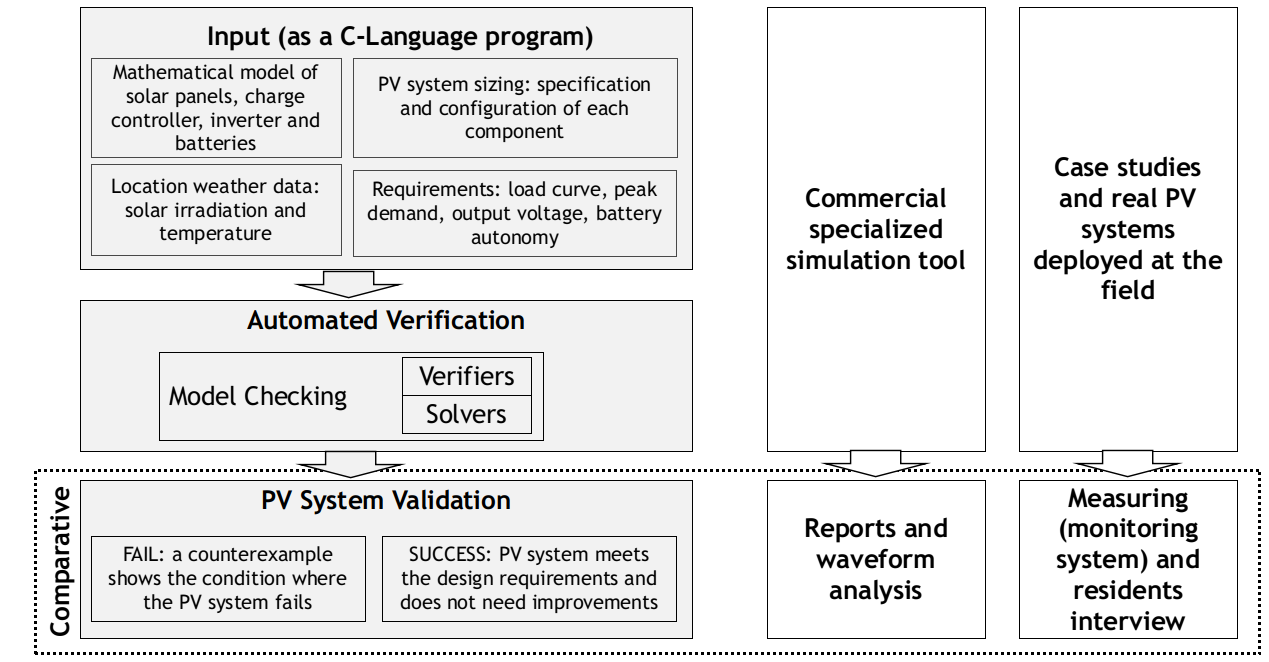
\includegraphics[width=0.85\textwidth]{verification_outline3.png}
\centering
\caption{Proposed validation of PV systems via automated verification.}
\label{fig:validation_outline} 
\end{figure}


\begin{figure}[h]
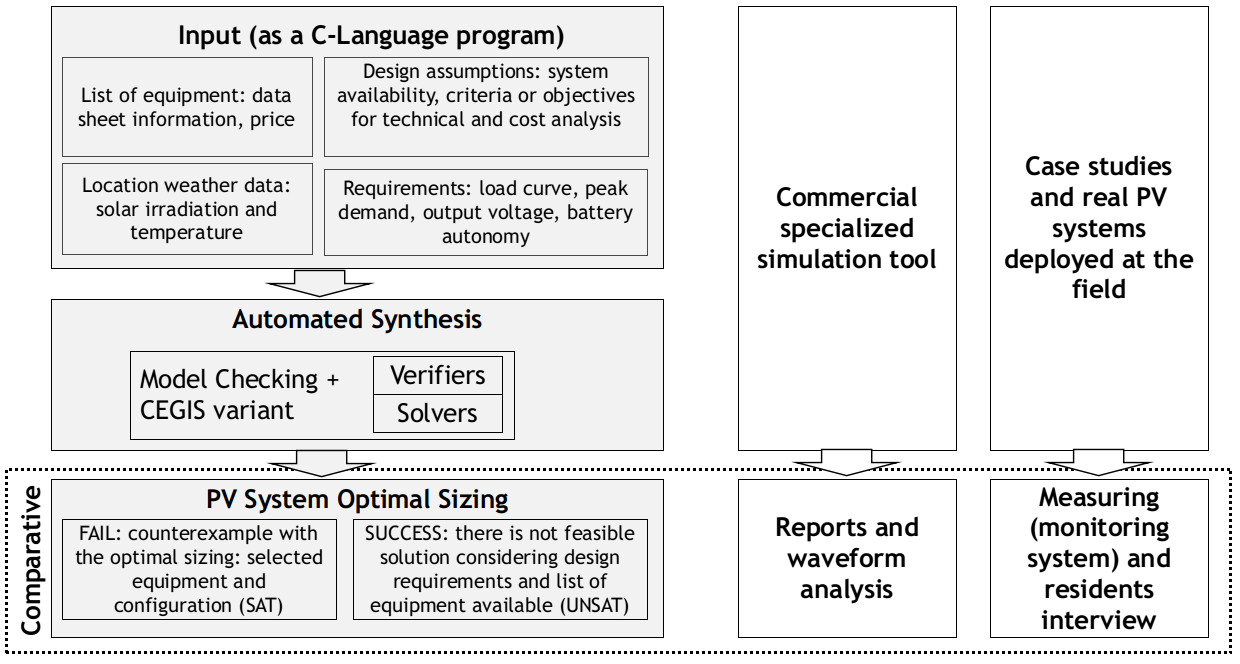
\includegraphics[width=0.85\textwidth]{optimization_outline3.png}
\centering
\caption{Proposed optimal sizing of PV systems via automated synthesis.}
\label{fig:optimization_outline} 
\end{figure}

Note that it is out of our scope to perform code modification on the verifiers or the solvers used during the automated verification or automated synthesis steps of our approach. Here we intend to create front-end applications for the verifiers and solvers (which are the back-end). That decision is based on the fact that we can be verifier-independent, and evaluate different back-ends, now and in the future, always searching for the best performance and soundness.

%----------------------------------------------
\section{Contributions}
%----------------------------------------------

\textcolor{red}{My comment: paragraphs broken in small and organized parts:}

Concerning the proposed \textbf{automated verification} technique, this thesis makes three main contributions: 
\begin{itemize}
\item \textbf{First}, we propose an algorithm written in the C programming language which implements the automated verification method to formally check the sizing and the operation of a given stand-alone PV system; 
\item \textbf{Second}, we evaluate the verification technique by comparing three state-of-the-art model checkers in five real case studies; and 
\item \textbf{Third}, experimental results show that this approach can find subtle design errors in stand-alone PV systems not easily detected by other approaches based on simulation.
\end{itemize}

In the area of \textbf{automated synthesis}, our study makes a further three original contributions: 
\begin{itemize}
\item \textbf{First}, it is the first application of a sound and automated formal synthesis approach which can provide accurate results for optimal sizing of stand-alone PV systems; 
\item \textbf{Second}, we propose a variant CEGIS method of synthesis with striking differences of how the Synthesize and Verify phases from the original CEGIS work (without solution candidate vector and using an incremental and iterative loop to reach the optimal cost solution); and 
\item \textbf{Third}, experimental results in seven case studies show that our approach qualitatively outperforms state-of-the-art simulation tools: our solution is far more detailed and closer to real PV systems than solutions presented by simulation.
\end{itemize}

% Firstly, we describe a modular modeling of each component of a PV system by means of mathematical models that can be encoded into fragments of first-order theories supported by software model checkers. Secondly
%
%With respect to the proposed \textbf{automated verification} method, this thesis makes three main contributions. 
%\textbf{First}, we propose an algorithm written in the C programming language, which implements the automated verification method to formally check the sizing and the operation of a given stand-alone PV system. \textbf{Second}, we evaluate the verification method by comparing three state-of-the-art model checkers in five real case studies. \textbf{Third}, experimental results show that this proposed approach can find subtle design errors in stand-alone PV systems, which are not easily detected by other approaches based on simulation. 
%
%The framework provided at this paper outlines the requirements, the process and the mathematical modeling to perform automated formal verification of a stand-alone PV system, using the satisfiability modulo theories (SMT)-based verification method.
%
%And linked to \textbf{automated synthesis}, our work makes more three original contributions: \textbf{First}, it is the first application of a sound and automated formal synthesis approach, which can provide accurate results of optimal sizing of stand-alone PV systems; \textbf{Secondly}, we propose a variant CEGIS method of synthesis with striking differences of how the {\sc Synthesize} and {\sc Verify} phases from original CEGIS work (without solution candidate vector and using an incremental and iterative loop to reach the optimal cost solution); and \textbf{Thirdly}, experimental results with seven case studies show that our approach qualitatively outperforms state-of-the-art simulation tool: our solution is far detailed and closer to real PV systems than the solution presented by simulation.
%
%three major contributions. 
%\textbf{First}, the use of automated symbolic verification methods in electrical systems was uncommon in recent prior studies~\cite{abs-1811-09438}, and specifically their use in synthesizing optimal PV sizing is unprecedented. Here, a list of PV components (i.e., PV panels, charge controllers, inverters, and batteries) can be fed to the proposed synthesis method together with the user requirements and environment constraints, and the proposed synthesis algorithm based on symbolic model checking can find the optimal solution in technical and economical terms. 
%\textbf{Second}, we evaluate different state-of-art symbolic software verifiers with the goal of obtaining the best performance in the verification back-end for synthesizing optimal PV systems, thereby being the first work that performs this type of evaluation. 
%\textbf{Third}, the experimental results show that the proposed synthesis method is an effective and efficient approach on the pursuit of the optimal solution of PV systems using formal methods, which outperforms existing state-of-the-art simulation tool. As a result, this thesis marks the first application of a sound and automated formal synthesis approach able to provide accurate results of optimal sizing of stand-alone PV systems. Thus, this research considerably advances the state-of-the-art in applied energy over the last two decades with the goal of optimally designing PV systems.
 
%---------------------------------------------- 
\section{Related Work}
%----------------------------------------------

In this section, we discuss only the use of formal methods in electrical systems in general since the optimization of PV sizing is currently not obtained by formal methods or even program synthesis. %Here we discuss only the use of formal methods on electrical systems in general since currently there exists no use of it or even program synthesis to obtain the optimization of PV sizing.

The conversion of the traditional power grid into a smart grid, a fundamental example of a CPS, raises many issues that require novel methods and applications. In $2012$, a Chinese smart grid implementation was considered as a case study to address the verification problem for performance and energy consumption~\cite{Yukseletall2012}. The authors employed a stochastic model checking approach and presented a modeling and analysis study using PRISM, which is a probabilistic model checker~\cite{KwiatkowskaNP11}. The focus of this study was on how CPSs integrate information and communication technology functions to the physical elements of a system for monitoring and controlling purposes. The authors did not focus on power generation or even solar PV systems.

In $2015$, an automated approach for applying Monte-Carlo simulation to power system protection schemes presented limitations of incomplete coverage of all possible operating conditions~\cite{Sengupta2015}. The authors proposed an automated simulation-based verification technique to verify the correctness of protection settings efficiently using a hybrid automata-temporal-logic framework. The initial focus was on relay operations and test-case generation to ensure the early detection of design errors. However, this study was limited to power system protection and did not deal with electricity generation or even solar PV systems.

Other related studies from $2015$ include a framework named Modana to achieve an integrated process from modeling with SysML/MARTE to analysis using statistical model checking for CPS in terms of non-functional properties such as time and energy~\cite{Cheng2015}. In order to demonstrate Modana's capability, the authors modeled energy-aware buildings as a case study and discussed the analysis of energy consumption in different scenarios. The focus here is on smart buildings and HVAC (heating, ventilation, and air conditioning) systems. This research, however, did not address the design and verification of solar PV systems. 
 
In $2017$, a researcher suggested the application of formal methods to verify and control the behavior of computational devices, interacting over a shared and smart infrastructure~\cite{Abate2017}. The author discussed the aggregation of large populations of thermostatically-controlled loads and PV panels, and the similar problems of energy management in smart buildings, of demand-response on smart grids, and respectively of frequency stabilization and grid robustness. The focus was on controlling the behavior of components, thereby verifying the given smart grid as a ``system of systems'' within the context of "internet of things". The author, however, used an approximate model checking of stochastic and hybrid models.

In $2018$, a verification methodology was proposed for the Cyber-Physical Energy Systems (CPES) with applications to PV panels and its distributed powerpoint tracking~\cite{Driouich2018}. This approach relied on representing the unpredictable behavior of the environment to cover all possible feasible scenarios. The simulation results obtained by JModelica covered the system's complete dynamic behavior; however, almost three days of computer effort to verify the design space of a single operational hour of the PV panels’ behavior made it clear that time was an issue. This related study did not include any other components of a stand-alone solar PV system. %however, it was evident the time-consuming issue with almost three days of computer effort to verify the design space of one operation hour of the PV panels behavior. This related study did not include other components of a stand-alone solar PV system.

Another study from $2018$ presented an approach to modeling smart grid components using a formal specification. The authors used a state-based formal specification language named Z; they demonstrated the application of Z to four smart grid components~\cite{Akram2018}. The formal specification presented can be considered a first step towards modeling smart grids using formal methods. The starting point of this study was that a smart home could be considered an integrated system consisting of various objects and systems, which communicate and interact with each other. This approach is based on Petri nets and works under the assumption that modeling smart homes lead to a clear understanding of the overall behavior of the smart grids.

However, prior studies did not deal with formal verification of a complete stand-alone PV system (with batteries, charge controller, and power inverter) or even solar PV systems optimization. Formal methods based on \textit{symbolic model checking} and its application to synthesize PV systems are still unexplored in the literature. Moreover, it is precisely on these gaps that this thesis is focused on.

%----------------------------------------------
\section{Thesis Organization}
%----------------------------------------------

This introduction has outlined the context, motivation, and problem addressed by this thesis and the objectives, solutions, and contributions of the research. The remaining chapters are organized as follows:

Chapter `~\nameref{chap:background}' presents the theoretical basis of formal methods, formal verification, automated verification, solar PV systems, design and validation of PV systems, program synthesis, and the mathematical modeling. 

Chapter `~\nameref{chap:automatedverification}' presents the automated formal verification technique, the experimentation details, and the results obtained with the tool created using this new method of PV systems validation. 

Chapter `~\nameref{chap:automatedsynthesis}' presents the automated synthesis technique from computer science and its application to obtain the optimal sizing of stand-alone solar PV systems, with details of the experimentation, and the results using the tools created to compare this new technique with a simulation tool and from data collected from fieldwork. 

In the `~\nameref{chap:conclusions}', we present the main contributions, future work directions and concluding remarks.

~\autoref{chap:publications} presents a list of papers that we submitted to international journals and conferences on the topic of the automated verification method. It covers the years 2015-2019, restricted to the Ph.D. process.

~\autoref{chap:tools} depicts the tools created during the Ph.D. process to implement and validate the two scientific methods of the thesis (and instructions for their use).

~\autoref{chap:data} presents detailed data from all the equipment used during the experimental part of the thesis, covering information from data-sheet, electrical features, brands, and models. 

It is worth mentioning that we decided, with the consent of the coordination of the graduate program, that this document would be written in the active voice and entirely in English. The choice of the active voice comes from the choice of the English language, which in the thesis studied was always presented in the active voice. The decision to use the English language stems from the possibility that the research may lead to further developments and activities, in the possibility of reaching a more significant number of people and helping in the internationalization of the Federal University of Amazonas.

\chapter{Background}
\label{chap:background}
In this chapter we present some concepts related to the intersection of the two areas:  computer science methods used to solve electrical engineering problems; in this case, the use of formal verification methodology to perform automated verification and optimal sizing of stand-alone solar PV systems.

First, we introduce the concept of formal verification as background to understanding how a methodology that performs (mainly) bug detection can be used to validate a design sizing or to obtain an optimal solution of PV systems.

And secondly, how a solar PV system can be modeled in order to be validated or optimized by formal verification methodology.

%%%%%%%%%%%%%%%%%%%%%%%%%%%%%%%%%%%%%%%%%%%%%%%%%%%%%%%%
\section{Formal Methods, Formal Design and Formal Verification}
%%%%%%%%%%%%%%%%%%%%%%%%%%%%%%%%%%%%%%%%%%%%%%%%%%%%%%%%

Formal methods are system design techniques that use rigorously specified mathematical models to validate systems, most notably (and known for) software and hardware systems~\cite{Collins98}. In contrast to other design systems, formal methods use mathematical proof as a complement to system testing in order to ensure correct behavior. With increasing scale and complexity, when safety becomes a more important issue, the formal approach to system design offers a better level of insurance.

Formal methods differ from other design systems through the use of formal verification schemes; the basic principles of the system must be proven correct before they are accepted~\cite{Bowen93}. Traditional system design has used extensive testing to verify behavior, but testing is capable of only finite conclusions. Dijkstra and others have demonstrated that tests can only show the situations where a system will not fail, but can say nothing about the behavior of the system outside of the testing scenarios~\cite{Bentley99}. In contrast, a theorem once proven true remains true.

Prior to the 1980s, mainly deductive verification was used as the formal method, with the use of axioms and proving rules to demonstrate the correctness of the system. The original focus was to verify critical systems based on the premise that if the system is important, time must be spent to verify it~\cite{Lowry1998}. Originally, formal methods were performed by hand.

It is worth pointing out that formal verification does not avoid the need for testing~\cite{Bowen95}. Formal verification can not correct bad assumptions in the design, but it can help to identify errors in reasoning which would otherwise be left unverified. In several cases, engineers have reported finding flaws in systems following a formal review of their designs~\cite{Kling95}.

A formal design can be summarized as a three step process, as described below~\cite{Collins98}:

\begin{itemize}
\item Formal Specification: During the formal specification phase, the engineer rigorously defines a system using a modeling language. Modeling languages are fixed grammars which allow users to model complex structures from predefined types (that are rigorously defined). This process of formal specification is similar to the process of converting a word problem into algebraic notation and helps engineers to clearly define their problems, goals and solutions. Several engineers who have used formal specifications claim that the clarity that this stage produces is a benefit in itself~\cite{Kling95}.
\item Verification: As stated above, formal methods differ from other specification systems by their heavy emphasis on provability and correctness. In building a system using formal specification, the designer is actually developing a set of theorems about his system. By proving these theorems correct, the formal verification ensures that the modeled system has an intended behavior. Verification is a difficult process, largely because even the simplest system has several dozen theorems, each of which has to be proven. Given the demands of complexity and Moore's law, almost all formal systems use an automated theorem proving tool of some form~\cite{Collins98}. That is the origin of 'automated verification' definition. These tools can prove simple theorems, verify the semantics of theorems, and provide assistance for verifying more complicated proofs, with feedback about the trace of the error (in order to correct the system and the specification of it).
\item Implementation: Once the model has been specified and verified, it is implemented by converting the specification into code.

\end{itemize}

%Formal methods are viewed with a certain degree of suspicion. While formal methods research has been progressing since 1960's, formal methods are only being slowly accepted by engineers. There are several reasons for this, but most of the problems seem to be a result of misapplication. Most formal systems are extremely descriptive and all-encompassing, modeling languages have generally been judged by their capacity to model anything. Unfortunately, these same qualities make formal methods very difficult to use, especially for engineers untrained in the type theory needed for most formal systems.[Bowen93]
%
%Conversely, it is apparent that some form of formal specification is necessary: complex systems require formal models. In addition,the mathematics required for formal methods is becoming a more prominent fixture of engineering curricula, engineering schools in Europe are already requiring courses in VDM, Z and similar formal specifications. Ultimately, formal methods will acquire some form of acceptance, but compromises will be made in both directions: formal methods will become simpler and formal methods training will become more common.
%
%Key Concepts
%Provability And Automated Verification
%Formal methods are distinguished from other specification systems by their emphasis on correctness and proof, which is ultimately another measure of system integrity. Proof is a complement, not a substitute, for testing. Testing is an important part of guaranteeing any system's fitness, but it is finite. Testing cannot demonstrate that a system operates properly; it can only demonstrate that the system works for the tested cases. Because testing cannot demonstrate that the system should work outside the tested cases, formal proof is necessary.
%
%Formally proving computer systems is not a new idea. Knuth and Dijkstra have written extensively on the topic, although their methods of proof are based on the traditional mathematical methods. In pure sciences, proofs are verified through extensive peer review before publication. Such techniques are time-intensive and less than perfect; it isn't unusual for a published proof to contain a flaw. Given the cost and time requirements of systems engineering, traditional proving techniques are not really applicable.
%
%Because of the costs of hand verification, most formal methods use automated theorem proving systems to verify their designs. Automated theorem provers are best described as mathematical CAD tools: they can prove simple propositions and automatically and provide assistance for verifying more complex theorems.
%
%Benefits Of Formal Models
%Formal methods offer additional benefits outside of provability, and these benefits do deserve some mention. However, most of these benefits are available from other systems, and usually without the steep learning curve that formal methods require.
%
%Discipline: By virtue of their rigor, formal systems require an engineer to think out his design in a more thorough fashion. In particular, a formal proof of correctness is going to require a rigorous specification of goals, not just operation. This thorough approach can help identify faulty reasoning far earlier than in traditional design.[Bowen95]
%The discipline involved in formal specification has proved useful even on already existing systems. Engineers using the PVS system, for example, reported identifying several microcode errors in one of their microprocessor designs.[Miller95]
%
%Precision: Traditionally, disciplines have moved into jargons and formal notation as the weaknesses of natural language descriptions become more glaringly obvious. There is no reason that systems engineering should differ, and there are several formal methods which are used almost exclusively for notation.[Bowen93]
%For engineers designing safety-critical systems, the benefits of formal methods lie in their clarity. Unlike many other design approaches, the formal verification requires very clearly defined goals and approaches. In a safety critical system, ambiguity can be extremely dangerous, and one of the primary benefits of the formal approach is the elimination of ambiguity.[Kling94].
%
%Weaknesses Of Formal Methods
%: Bowen points out that formal methods are generally viewed with suspicion by the professional engineering community, and the propensity of tentative case studies and advocacy papers for the formal approach would seem to support his thesis [Bowen93]. There are several reasons why formal methods are not used as much as they might be, most stemming from overreaching on the part of formal methods advocates.
%Expense:Because of the rigor involved, formal methods are always going to be more expensive than traditional approaches to engineering. However, given that software cost estimation is more of an art than a science, it is debatable exactly how much more expensive formal verification is. In general, formal methods involve a large initial cost followed by less consumption as the project progresses; this is a reverse from the normal cost model for software development.[Bowen93]
%
%Limits Of Computational Models:While not a universal problem, most formal methods introduce some form of computational model, usually hamstringing the operations allowed in order to make the notation elegant and the system provable. Unfortunately, these design limitations are usually considered intolerable from a developer's perspective.
%An excellent example comes from SML. Statements of proof in SML depend on a purely functional programming model: all data is passed through the parameter/return mechanism of a function, no side effect alterations, modifications of global variables or the like is allowed [Paulson96]. Handling side effects and other aberrancies are a requirement for any system involving input, network operations or other systems which require interrupts, meaning that SML's model is, to some extent, broken.
%
%Usability:Traditionally, formal methods have been judged on the richness of their descriptive model. That is, 'good' formal methods have described a wide variety of systems, and 'bad' formal methods have been limited in their descriptive capacities. While an all-encompassing formal description is attractive from a theoretical perspective, it invariably involved developing an incredibly complex and nuanced description language, which returns to the difficulties of natural language. Case studies of full formal methods often acknowledge the need for a less all-encompassing approach.[Miller95]
%Arguably, many of these failures can be attributed to overreaching on the part of formal methods advocates. This reasoning has led to the lightweight approach to formal specification.
%
%The Lightweight Approach
%The flaws in formal specifications have been heavily focused on in the past few years, leading to several alternate approaches. The traditional view of formal methods as all-encompassing highly abstracted schemes has led to formal methods being all-encompassing, extremely rigorous, and very expensive. While theoretically appealing, formal methods have generally been ignored by engineers in the field.
%The lightweight approach to formal design recognizes that formal methods are not a panacea: there are areas where formal methods are useful, and areas where a formal specification will accomplish nothing. In a lightweight design, formal methods are used in specific locations, and different formal methods may be used in different subsystems, ideally playing to the strengths of each method [Easterbrook 98]. In such a system, Petri Nets might be used to describe the communications protocol, and a LARCH system might be used to model the data storage. For other parts of the system, formal specifications might be avoided entirely: for example, the user interface may be refined using a rapid prototyping system and client interviews.
%
%The lightweight approach is a traditional engineering compromise, and there is a tradeoff. As formal methods become more common, engineers will have to learn type theory, modern algebra and proof techniques. Ultimately, engineers will have to think more like mathematicians.

%%%%%%%%%%%%%%%%%%%%%%%%%%%%%%%%%%%%%%%%%%%%%%%%%%%%%%%%
\section{Project Validation, Automated Verification and Synthesis Using Model Checking}
\label{sec:AutomatedVerification}
%%%%%%%%%%%%%%%%%%%%%%%%%%%%%%%%%%%%%%%%%%%%%%%%%%%%%%%%

%\section{Automated Verification }
It is necessary to keep in mind that validation is the process of determining whether a design meets the needs of the user, whereas verification is the process of determining whether a design meets a set of requirements, specifications, and regulations.  

If the requirements, specifications, and regulations are given in a formal language, then it may be possible to automate verification.  

Simulation may also be used for validation, but it raises more problems for verification. In order to use simulation for verification, it is necessary to ensure adequate coverage of operating conditions, scenarios, and system inputs. Testing can also be used for validation, but for the same reasons, it too raises problems for verification.
 
According to \cite{Clarke2008}, verification procedure is an intelligent exhaustive search of the state space of the design. In addition, according to \cite{Forejt2011}, formal verification is a systematic approach that applies mathematical reasoning to obtain guarantees about the correctness of a system. One successful method in this domain is model checking.

\subsection{Model Checking}
  
Model checking is an automatic verification technique, as defined by \cite{Clarke2008}. Model checking was originally developed for reasoning about finite state of concurrent systems, though nowadays it is mainly used for hardware and software verification, but can be applied to any kind of system. 

The process of model checking can be divided in three components: modeling, specification, and verification method. 

\begin{itemize}
\item In modeling, a model (normally mathematical) of the system is created; 
\item In specification, normally a list of properties to be satisfied by the system is established, i.e., the requirements, such as reliability to performance, for example; 
\item Normally it is expressed in temporal logic form ($CTL$); 
\item The model checking is the verification method itself. 
\end{itemize}

The model checking algorithm can be described as:  

\begin{itemize}
\item Given the model $ 'M' $ and a $CTL$ formula $ \phi $ as input;  
\item The moodel checking algorithm provides all the states of model $ M $ which satisfy $ \phi $;  
\item It returns $YES$ if $ \phi $ is $TRUE$, or returns $NO$ if $ \phi $ is $FALSE$.  

\end{itemize}
Specifically, in the case of $ \phi $ being $FALSE$, the algorithm returns a counterexample that is useful as a system diagnostic, in order to discover in which situation the model has been violated. \cite{Clarke2008} considers this to be the most important advantage of model checking.  
 
Model checking presents several other advantages: proofs are not needed (the algorithm is not a deductive procedure); there is no problem with partial specifications of the system, logics can easily express many concurrency properties; it is fast (compared to other rigorous methods such as interactive theorem proving). However, there is one major disadvantage in model checking: the state explosion problem. 

The model checking problem can be defined as shown in \cite{Clarke2008}: 

\begin{itemize}
\item Let $M$ be a Kripke structure (i.e., a state transition graph);
\item $f$ be the specification in temporal logic (a formula);
\item Find all states $s$ of $M$ such that $M , s \models f$
\end{itemize}

Fig. \ref{fig:modelcheckstruc} shows the structure of a typical model checking system. A preprocessor extracts a state transition graph from a system (program or circuit).

\begin{figure}[h]
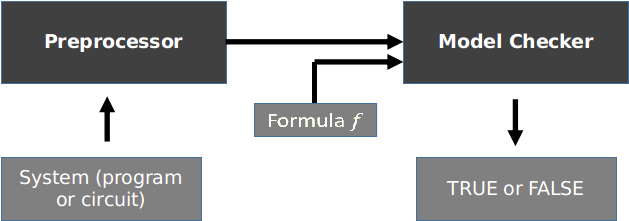
\includegraphics[width=0.8\textwidth]{modelcheckstruc}
\centering
\caption{Model Checker structure. Source: \cite{Clarke2008}.}
\label{fig:modelcheckstruc}
\end{figure}

Here it is worth mentioning that the term "model" is not used here with its dictionary definition. In other words, the problem is not dealing with an abstraction of the actual system under study. 

The Fig. \ref{fig:systemverif} shows the process of converting a real system to a model in order to be verified by model checking. 

\begin{figure}[h]
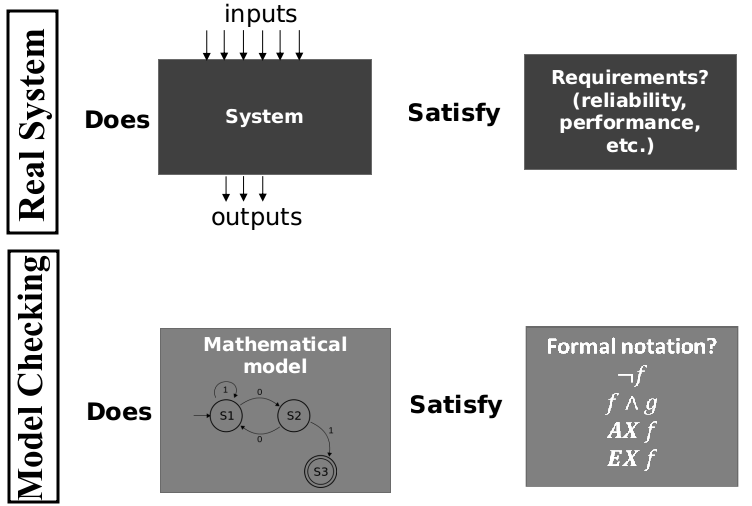
\includegraphics[width=0.8\textwidth]{systemverif3}
\centering
\caption{From real system verification to model checking. Source: adapted from \cite{Clarke2008}.}
\label{fig:systemverif}
\end{figure}

In order to solve the problem of state explosion, many different techniques have been developed over the last decades. One of the most promising is Bounded Model Checking (BMC). 

BMC is a method that checks the model up to a given point in the path length. The BMC algorithms traverse a finite state machine for a fixed number of steps, $k$, and check whether violation occurs within this bound. It uses fast SAT solvers, where SAT means satisfiability. 

A SAT problem, as defined by \cite{Clarke2008}, is a problem of determining if there are certain conditions or interpretations that satisfy a given Boolean expression. SAT solvers are used in BMC, such that if there is some Boolean function, the solver would search the model for conditions (value of variables) that would make the formula $TRUE$. If the SAT Solver finds a substitution for the formula/function then the substitute induces a counterexample.  

%%CBMC is considering the best-known model verification tool to validate code in ANSI-C and C++, as can be seen in \cite{Kroening}. 
%
%ESBMC is a context-bounded model checker for embedded C/C++ software based on Satisfiability Modulo Theories (SMT) solver, which can use CBMC as front-end.  
The use of SMT, instead of Boolean Satisfiability SAT from the original BMC, comes as an alternative to overcome limitations of the system's modeling, especially considering that the complexity of these is increasing and the SMT method has a higher level and richer theories than the SAT to represent the models. 

%Although simulation and testing explore possible behaviors and scenarios of a given system, they leave open the question of whether unexplored trajectories may contain a flaw~\cite{ClarkeHV18}. Formal verification conducts an exhaustive exploration of all possible behaviors; when a design is said to be ``correct'' by a formal verification method, it implies that all behaviors have been explored; questions regarding adequate coverage or missed behavior becomes irrelevant~\cite{Clarke2012}. Formal verification is a systematic approach that applies mathematical reasoning to obtain guarantees about the correctness of a system; one successful method in this domain is model checking~\cite{Clarke2012}. 

In this study we will evaluate three state-of-the-art model checkers to formally verifying and synthesize PV designs w.r.t. user requirements. In addition, other solvers will be evaluated, according to the feature of each model checker.

%%%%%%%%%%%%%%%%%%%%%%%%%%%%%%%%%%%%%%%%%%%%%%%%%%%%%%%%
\subsection{CBMC}
%%%%%%%%%%%%%%%%%%%%%%%%%%%%%%%%%%%%%%%%%%%%%%%%%%%%%%%%

The C Bounded Model Checker (CBMC) falsifies assertions in C programs or proves that they are safe if a completeness threshold is given~\cite{Kroening}. CBMC implements a bit-precise translation of a C program, annotated with assertions and with loops unrolled up to a given depth, into a logical formula. If the formula is satisfiable, then a failing execution that leads to a violated assertion exists~\cite{Kroening}. 

CBMC's verification flow can be summarized in three stages: 

\begin{itemize}
\item Front-end: scans, parses and type-checks C code; it converts control flow elements, such as \textit{if} or \textit{switch} statements, loops and jumps, into equivalent guarded \textit{goto} statements, thus aiming to reduce verification effort; 
\item Middle-end: performs symbolic execution by eagerly unwinding loops up to a fixed bound, which can be specified by the user on a per-loop basis or globally, for all loops and finally; 
\item Back-end: supports SAT and SMT solvers to discharge verification conditions.
\end{itemize}

Specifically, CBMC comes with a built-in solver for bit-vector formulas that is based on MiniSat. We used this solver during the experimentation in this Ph.D thesis~\cite{Kroening}.

%%%%%%%%%%%%%%%%%%%%%%%%%%%%%%%%%%%%%%%%%%%%%%%%%%%%%%%%
\subsection{ESBMC}
%%%%%%%%%%%%%%%%%%%%%%%%%%%%%%%%%%%%%%%%%%%%%%%%%%%%%%%%

The Efficient SMT-based Bounded Model Checker (ESBMC) is a bounded and unbounded model checker for C~\cite{esbmc2018}, C++~\cite{RamalhoFSMC013}, Qt~\cite{MonteiroGCF17}, and CUDA~\cite{PereiraASMMFC17} programs, which supports the verification of LTL properties with bounded traces~\cite{DBLP:journals/sosym/MorseCN015}. 

ESBMC's verification flow can be summarized in three stages: 

\begin{itemize}
\item A front-end that can read and compile C code, where the system's formal specification is first handled; 
\item Preprocessing steps deal with code representation, control flow and unwinding of loops, and model simplification, thereby aiming to reduce verification effort; and finally 
\item The SMT solving stage, where all constraints and properties of the system are encoded into SMT and checked for satisfiability.
\end{itemize}
 
ESBMC exploits the standardized input language of SMT solvers (SMT-LIB\footnote{http://smtlib.cs.uiowa.edu/} logic format) to make use of a resource called \textit{assertion stack}~\cite{Morse2015}. This enables ESBMC, and the respective solver, to learn from previous checks, thus optimizing the search procedure and potentially eliminating a large amount of formula state space to be searched, because it solves and disregards data during the process, incrementally. This technique is called 'incremental SMT'~\cite{DBLP:journals/fac/SchrammelKBMTB17} and allows ESBMC to reduce the memory overhead, mainly when the verified system is complex and the computing platform does not have a large amount of memory to deal with the entire design space state. ESBMC in 'incremental SMT' uses only the Z3 solver~\cite{DeMoura}.

%%%%%%%%%%%%%%%%%%%%%%%%%%%%%%%%%%%%%%%%%%%%%%%%%%%%%%%%
\subsection{CPAchecker}
%%%%%%%%%%%%%%%%%%%%%%%%%%%%%%%%%%%%%%%%%%%%%%%%%%%%%%%%

Automatic program verification requires a choice between precision and efficiency. The more precise a method, the fewer false positives it will produce, but also the more expensive it is, and thus applicable to fewer programs. 

Historically, this trade-off was reflected in two major approaches to static verification: program analysis and model checking. In order to experiment with the trade-off, and in order to be able to set the dial between the two extreme points, Configurable Program Analysis (CPA) provides a conceptual basis for expressing different verification approaches in the same formal setting. 

CPA formalism provides an interface for the definition of program analyses. Consequently, CPAchecker provides an implementation framework that allows the seamless integration of program analyses that are expressed in the CPA framework. The comparison among different approaches in the same experimental setting is intended to be easy and the experimental results are expected to be more meaningful~\cite{Beyer2011}. As to the architecture, the central data structure is a set of control-flow automata (CFA), which consists of control-flow locations and control-flow edges. 

The CPA framework provides interfaces to SMT solvers and interpolation procedures~\cite{Beyer2011}. Currently, CPAchecker uses MathSAT as SMT solver; and CSIsat and MathSAT as interpolation procedures~\cite{Beyer2011}. %CPAchecker performs reachability analysis and operates on an object of the abstract data type CPA, i.e., the underlying verification algorithm applies operations from the CPA interface without knowing which concrete CPA it is analyzing. For most configurations, the concrete CPA will be a composite CPA, which implements the combination of different CPAs. \textcolor{red}{It is unclear what a CPA is.}
%In software verification, it is usual to take a considerable amount of effort to convert a verification idea into actual experimental results and CPAchecker aims to accelerate this process~\cite{Beyer2011}.

%-----------------------------------------------------------
\subsection{CEGIS and Program Synthesis}
\label{sec:ProgramSynthesis}
%-----------------------------------------------------------

Program synthesis addresses an age-old problem in computer science: can a computer program itself?~\cite{Bornholt2019}. Before the computer can automatically generate a program, it is necessary to give it a specification of what the program should do. The specification needs to describe the program's desired behavior to ensure that the program does what it is intended.

The basic idea of program synthesis is to automatically construct a program $P$ that satisfies a correctness specification $\sigma$. In particular, program synthesis is automatically performed by engines that use a correctness specification $\sigma$ as starting point, and then incrementally produce a sequence of candidate solutions that partially satisfy $\sigma$~\cite{Abateetal2017}. As a result, a given candidate program $p$ is iteratively refined, in order to match $\sigma$ more closely. 

CEGIS represents one of the most popular approaches to program synthesis that are currently in use for CPS~\cite{Abateetal2017}, whose basic architecture is illustrated in Figure~\ref{Counter-Example-Guided-Inductive-Synthesis} and has close connections to algorithmic debugging using counterexamples and abstraction refinement~\cite{Alur}. 

\begin{figure}[h]
	\centering
	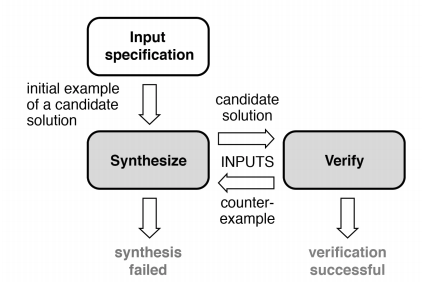
\includegraphics[width=0.75\columnwidth]{fig2_orig}
	\caption{Counterexample Guided Inductive Synthesis (CEGIS).}
	\label{Counter-Example-Guided-Inductive-Synthesis}
\end{figure}

The correctness specification $\sigma$ provided to our program synthesizer is of the form $\exists \vec{F} .  \forall \vec{x}.  \sigma(\vec{x}, \vec{F})$, where $\vec{F}$ ranges over functions, $\vec{x}$ ranges over ground terms, and $\sigma$ is a quantifier-free (QF) formula typically supported by SMT solvers. The ground terms are interpreted over some finite domain $\mathcal{D}$, where $\mathcal{D}$ can be encoded using the SMT's bit-vectors part. 

In Figure~\ref{Counter-Example-Guided-Inductive-Synthesis}, the  CEGIS method's {\sc Synthesize} and {\sc Verify} phases interact via a finite set of test vector {\sc inputs}, which is incrementally updated. Given the correctness specification $\sigma$, the {\sc Synthesize} procedure tries to find an existential witness $\vec{F}$ satisfying the specification $\sigma(\vec{x}, \vec{F})$, for all $\vec{x}$ in {\sc inputs} (as opposed to all $\vec{x} \in \mathcal{D}$). If {\sc Synthesize} succeeds in finding a witness~$\vec{F}$, the latter is a candidate solution (i.e., a feasible combination of equipment) for the full synthesis formula, which is passed to {\sc Verify} in order to check whether it is a proper solution ({\it i.e.}, $\vec{F}$ satisfies the specification $\sigma(\vec{x}, \vec{F})$ for all $\vec{x}\in\mathcal{D}$). If this is the case, then the algorithm terminates, i.e., we have found a feasible solution; otherwise, in the CEGIS method, additional information is provided for the {\sc Synthesize} phase, in the form of a new counterexample that is added to the {\sc inputs} set and the loop iterates again.

One may notice that each iteration of the CEGIS loop adds a new input to the finite set $\text{\sc inputs}$, which is then used for synthesis.  Given that the full set of inputs $\mathcal{D}$ is finite because we use bit-vector expressions, this means that the refinement loop can only iterate over a finite number of times. However, {\sc Synthesize} may conclude that no candidate solution obeying $\sigma$ for the finite set $\text{\sc inputs}$ exists and our synthesis engine can then conclude that no feasible solution was found.

\section{Solar Photovoltaic Systems}

According to \cite{Roy}, a PV system is designed to supply electrical loads. This load can be of the Alternating Current (AC) type or the Direct Current (DC) type. The supply electricity can be needed either in daytime or nighttime (in particular cases, in both). The most basic PV system can supply only in daytime.  For the night hours or rainy days, batteries are needed, where power can be stored and used \cite{Gules}. 

PV systems are broadly classified into three distinct types, as described by \cite{Mohanty}: 

\begin{itemize}
\item Standalone systems, where the energy is generated and consumed in the same place and which does not interact with the main grid. Normally, the electricity consuming/utilizing device is part of the system, i.e., solar home systems, solar street lighting systems, solar lanterns, and solar power plants; 
\item Grid-connected systems, where the solar PV system is connected to the grid. The grid-connected system can be either a grid-tied system, which can only feed power into the grid, with the result that this system cannot deliver power locally during blackouts and emergencies since these systems have to be completely disconnected from the grid and have to be shut down as per national and international electrical safety standards. Some grid-connected PV systems, with energy storage, can also provide power locally in an islanding mode; 
\item Solar PV hybrid systems: In a hybrid system, another source(s) of energy, such as wind, biomass or diesel, can work together with the solar PV system to provide the required demand. In this type of system, the main objective is to bring more reliability into the overall system at an affordable cost by adding one or more energy sources.
\end{itemize}
 
In the specific case of isolated communities, depending on the type of load, cost, resources availability, and the load requirements, standalone systems can be split into several categories, as described below. Since the goal of this Thesis is to present solutions only to isolated/ off-grid applications, on-grid or hybrid configurations are not discussed here.
 
There is a resource, called maximum power point tracking (MPPT), which is an electronic control mechanism that maintains the PV operating at a voltage that corresponds to maximum power voltage, which maximizes the transfer of power while avoiding loss of PV cells \cite{Pinho}. This resource is found in modern PV systems and is strongly indicated due to its advantages.

\subsection{Unregulated standalone PV systems with DC load }
Usually this type of system is for low power applications, as defined by \cite{Roy}. The PV system is directly connected to the load without any MPPT controller, as shown in Fig.\ref{fig:unregSPV}. At night, the system will not provide any supply because of the absence of a battery. 
 
\begin{figure}[h]
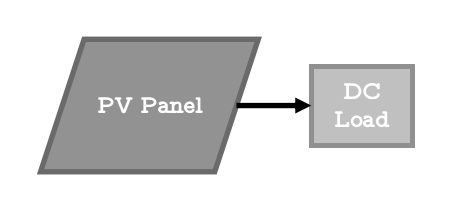
\includegraphics[width=0.6\textwidth]{unregulatedSPV.png}
\centering
\caption{Unregulated standalone SPV system with DC load. Source: \cite{Roy}.}
\label{fig:unregSPV}
\end{figure}

\subsection{Regulated standalone PV systems with DC load}
Similar to the unregulated standalone system with DC load, the main difference between this and the previous one is that this system requires a MPPT technique, as illustrated in Fig.\ref{fig:regSPV1}. Usually systems with MPPT should have a battery; otherwise, the extra power will be wasted.

\begin{figure}[h]
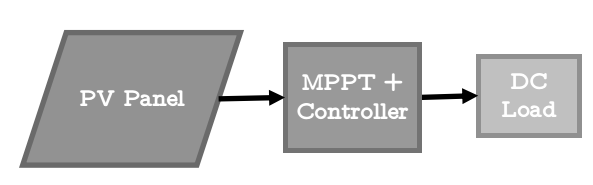
\includegraphics[width=0.8\textwidth]{regulatedSPV1.png}
\centering
\caption{Regulated standalone SPV system with DC load. Source: \cite{Roy}.}
\label{fig:regSPV1}
\end{figure}

%%%%%%%%%%%%%%%%%%%%%%%%%%%%%%%%%%%%%%%%%%%%%%%%%%%%%%%%
\subsection{Regulated standalone systems with battery and DC load}
%%%%%%%%%%%%%%%%%%%%%%%%%%%%%%%%%%%%%%%%%%%%%%%%%%%%%%%%

Configuration with PV array, battery, MPPT and DC load, as shown in Fig.\ref{fig:regSPV2}. The battery is used to store the extra power from the PV system. A charge controller is necessary for this type of system because the useful life of the battery is less than that of the PV module. Extra charging and deep discharging can reduce the battery life \cite{Kim}. 

\begin{figure}[h]
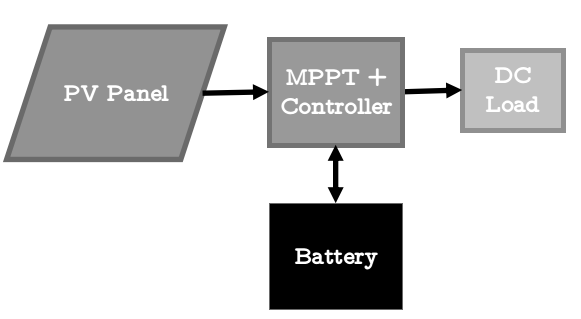
\includegraphics[width=0.8\textwidth]{regulatedSPV2.png}
\centering
\caption{Regulated standalone SPV system with battery and DC load. Source: \cite{Roy}.}
\label{fig:regSPV2}
\end{figure}

According to \cite{Pinho}, PV systems that are used to feed loads with low variation of consumption can be sized to operate without the controller. This is known as a self-regulated standalone PV system with battery. However, PV panel voltage must be compatible with the battery voltage. Normally, the bank of batteries is oversized in relation to the PV panel and to the load. The drawback is the operation of the batteries, normally overloaded or with excessive discharges (that can damage the batteries).

%%%%%%%%%%%%%%%%%%%%%%%%%%%%%%%%%%%%%%%%%%%%%%%%%%%%%%%%
\subsection{Regulated standalone systems with battery, AC load}
%%%%%%%%%%%%%%%%%%%%%%%%%%%%%%%%%%%%%%%%%%%%%%%%%%%%%%%%

This system is similar to the previous one, but the AC load draws the power from the PV system and, because of the AC load, an inverter (DC to AC converter) is required, as seen in Fig.\ref{fig:regSPV3}. This solution has an cost increase because it has more equipment. However, AC availability has the advantage of permitting the use of a higher number of AC appliances in homes or consumer units. This configuration is this thesis since it is currently the most common system used specifically for remote rural areas of developing countries or areas where the grid extension is not feasible.
%stand-alone systems are one the most used solutions, and 
% depending on the type of load, cost, resources availability, and requirements of the load, 
%stand-alone systems 
%can be split into several categories. However, 
%the most suitable configuration is the regulated stand-alone system with battery and AC load.

\begin{figure}[h]
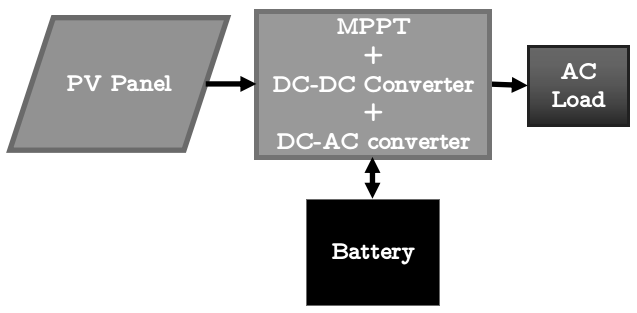
\includegraphics[width=0.8\textwidth]{regulatedSPV3.png}
\centering
\caption{Regulated standalone system with battery, AC load. Source: \cite{Roy}.}
\label{fig:regSPV3}
\end{figure}

%%%%%%%%%%%%%%%%%%%%%%%%%%%%%%%%%%%%%%%%%%%%%%%%%%%%%%%%
\subsection{Design and Validation of a Solar photovoltaic system}
%%%%%%%%%%%%%%%%%%%%%%%%%%%%%%%%%%%%%%%%%%%%%%%%%%%%%%%%

The design and validation of a SPV system can be done by hand or with the aid of a software tool. 

In order to address different aspects of a project system and system's design, a lot of public domain and commercial software is available for the SPV market. According to \cite{Brooks}, the capabilities of these tools range from simple solar resource and energy production estimation, to site survey and system design tools, and to complex financial analysis software (with optimization). Some tools also provide support to rebate program applications and tax incentives (specific to each country or region), while other programs and worksheets focus on the technical aspects of system sizing and design.
 
Manufacturers and integrators also have their own proprietary software to perform inverter string sizing and various system sizing and design tools, with the drawback of just including´ their own products among the possibilities of choice. In this study, the most widely used tools are presented: 

\begin{itemize}
\item PVWatts 
\item SAM
\item Homer
\item RETScreen
\item Hybrid2
\end{itemize}

%%%%%%%%%%%%%%%%%%%%%%%%%%%%%%%%%%%%%%%%%%%%%%%%%%%%%%%%
\subsubsection{PVWatts Calculator}
%%%%%%%%%%%%%%%%%%%%%%%%%%%%%%%%%%%%%%%%%%%%%%%%%%%%%%%%

According to \cite{Freeman} and \cite{NRELDobos}, this is a web application developed by the National Renewable Energy Laboratory (NREL), which estimates the electricity production of a grid-connected roof- or ground-mounted photovoltaic system based on a few inputs. According to \cite{NRELDobos}, using the calculator, requires information about the system's location, basic design parameters, and system economics. PVWatts calculates estimated values for the system's annual and monthly electricity production, and for the electricity's monetary value. This tool is suitable for very preliminary studies of a potential location for a photovoltaic system that uses crystalline silicon or thin film photovoltaic modules. The production estimates that PVWatts computation does not account for many factors that are important in the design of a photovoltaic system, which makes it necessary to have the support of an energy expert. The calculator estimates the monthly and annual electricity production of a photovoltaic system using an hour-by-hour simulation over a period of one year. To represent the system's physical characteristics, PVWatts requires values for six inputs: System DC size; Module type; Array type; System losses; Array tilt angle; Array azimuth angle.

%%%%%%%%%%%%%%%%%%%%%%%%%%%%%%%%%%%%%%%%%%%%%%%%%%%%%%%%
\subsubsection{SAM}
%%%%%%%%%%%%%%%%%%%%%%%%%%%%%%%%%%%%%%%%%%%%%%%%%%%%%%%%

SAM or System Advisor Model is a software solution produced by the U.S. Department of Energy and National Renewable Energy Laboratory. According to \cite{NRELBlair} and \cite{Cameron2008}, SAM is intended to help users to determine whether the model meets their project constraints/specifications, and (also) to provide information for readers who do not plan to use the model, but want to learn about its capabilities. SAM is a performance and financial model designed to facilitate decision making for people involved in the renewable energy industry: project managers and engineers; financial and policy analysts; technology developers; and researchers. SAM makes performance predictions and energy cost estimates for grid-connected power projects based on installation and operating costs and system design parameters that user specifies as inputs to the model. Projects can be either on the customer side of the utility meter, where they buy and sell electricity at retail rates, or on the utility side of the meter, where they sell electricity at a price negotiated through a power purchase agreement. SAM is an electrical power generation model and assumes that the renewable energy system delivers power either to an electric grid, or to a grid-connected building or facility to meet the electric load. It does not model thermal energy systems that meet a thermal process load. As mentioned in \cite{NRELBlair}, SAM does not model isolated or off-grid power systems, and does not model systems with electricity storage batteries.

%%%%%%%%%%%%%%%%%%%%%%%%%%%%%%%%%%%%%%%%%%%%%%%%%%%%%%%%
\subsubsection{HOMER}
%%%%%%%%%%%%%%%%%%%%%%%%%%%%%%%%%%%%%%%%%%%%%%%%%%%%%%%%

As defined in \cite{HOMER}, this is actually a set of two tools: HOMER Legacy and HOMER Pro. HOMER is an acronym for Hybrid Optimization Model for Multiple Energy Resources. HOMER Legacy is the original HOMER software version created at the National Renewable Energy Laboratory (NREL). HOMER Legacy is a free computer model that simplifies the task of evaluating design options for both off-grid and grid-connected power systems for remote, stand-alone, and distributed generation applications. HOMER's optimization and sensitivity analysis algorithms allow the user to evaluate the economic and technical feasibility of a large number of technology options. Since 2016 Homer Legacy can be found at the HOMER web site, but it is only available for students and nonprofit organizations, as defined in \cite{HOMER}, and has no support available. For a short-time only the commercial version will remain.
 
The commercial version (paid), known as HOMER Pro, as defined in \cite{Swarnkar}, is a tool for optimizing micro-grid design in all sectors, from village power and island utilities to grid-connected campuses and military bases. HOMER Pro puts together three tools in one product: optimization, simulation, and sensitivity analysis. It provides the detailed rigor of chronological simulation and optimization in a model that is intended to be easy to use and is adaptable to a wide variety of projects. For a village or community-scale power system, HOMER can model both the technical and economic factors involved in the project. For larger systems, HOMER can provide an overview that compares the cost and feasibility of different configurations. Chronological simulation is essential for modeling variable resources, such as solar and wind power and for combined heat and power applications, where the thermal load is variable. HOMER's sensitivity analysis helps determine the potential impact of uncertain factors such as fuel prices or wind speed on a given system. 

%%%%%%%%%%%%%%%%%%%%%%%%%%%%%%%%%%%%%%%%%%%%%%%%%%%%%%%%
\subsubsection{RETScreen}
%%%%%%%%%%%%%%%%%%%%%%%%%%%%%%%%%%%%%%%%%%%%%%%%%%%%%%%%

As mentioned in \cite{Pradhan}, RETScreen is a decision-support tool designed to help decision makers and energy professionals to evaluate the financial viability of renewable energy, energy efficiency, and/or co-generation projects.

RETScreen models various types of renewable energy technologies (RETs), allowing for comparisons between technology options. The software can be used to evaluate benefits from both clean energy production from power generation projects and savings through energy efficiency projects, accounting for project costs, greenhouse gas emission reductions, and financial risk. The software is freely distributed (but with restrictions to save work or print), and had three different versions:

\begin{itemize}
\item RETScreen 4 (discontinued, requires Microsoft Excel to run); 
\item RETScreen Software Suite, which includes the RETScreen 4 and a Windows-based graphical software that allows project owners to verify the ongoing energy performance of their facilities (discontinued in 2013);
\item And the current (2016) RETScreen Expert, which allows users to evaluate energy investments over an entire project life-cycle (including benchmarking, feasibility, and performance analysis) in a fully integrated way, and within one software platform. This version is only Windows-based and has a complete paid version, via annual subscription way.
\end{itemize}

As described by \cite{Pradhan}, RETScreen performs a standard five-step analysis: setting and site conditions; energy model; cost analysis; emission analysis, financial analysis, sensitivity, and risk analysis. It is developed and maintained by the Government of Canada, through the CanmetENERGY Varennes Research Centre of Natural Resources; in collaboration with: NASA; Renewable Energy and Energy Efficiency Partnership (REEEP); United Nations Environment Programme (UNEP), and the Global Environment Facility (GEF). RETScreen is available in 36 languages; it is a multi-awarded tool, and includes equipment databases for components manufactured and available worldwide.

%%%%%%%%%%%%%%%%%%%%%%%%%%%%%%%%%%%%%%%%%%%%%%%%%%%%%%%%
\subsubsection{Hybrid2}
%%%%%%%%%%%%%%%%%%%%%%%%%%%%%%%%%%%%%%%%%%%%%%%%%%%%%%%%

The Hybrid2 software package, as described in \cite{Mills}, is a user-friendly tool that executes detailed long-term performance and economic analysis on a wide variety of hybrid power systems. Hybrid2 is a probabilistic/time series computer model, using time series data for loads, wind speed, solar insolation, and temperature; and the power system is designed or selected by the user, in order to predict the performance of the hybrid power system. Variations in wind speed and in load within each time step are factored into the performance predictions. The code does not consider short-term system fluctuations caused by system dynamics or component transients. This program is not supported anymore and according to \cite{UMASS}, probably after the user performs the free download of the tool, it will not work on Windows platforms later than Windows XP, which is a limitation.

Table \ref{table:softwares} summarizes the tools described in this paper.  Where just Hybrid2 is mentioned, no technical support is available; only HOMER, RETScreen and Hybrid2 perform off-grid system or battery backup analysis; all the tools perform solar photovoltaic analysis; only HOMER and RETScreen are complete, including economic analysis and even optimization-sensitive analysis. However, only the paid version of these software packages have all the features, and they run only on Windows-based operating systems.

\begin{table}[!t]
%% increase table row spacing, adjust to taste
\renewcommand{\arraystretch}{1.3}
% if using array.sty, it might be a good idea to tweak the value of
% \extrarowheight as needed to properly center the text within the cells
\caption{Comparative coverage of reference softwares}
\label{table:softwares}
\centering
%% Some packages, such as MDW tools, offer better commands for making tables
%% than the plain LaTeX2e tabular which is used here.
\begin{tabular}{c | c | c | c | c | c}
\hline
\hline
Characteristic  & \rotatebox{90}{PVWatts} & \rotatebox{90}{SAM} & \rotatebox{90}{HOMER} & \rotatebox{90}{RETScreen } & \rotatebox{90}{Hybrid2}\\
\hline
Support & X & X & X & X &  \\
Off-grid systems &   &   & X & X & X\\
Hybrid systems &  &  & X & X & X\\
Photovoltaics & X & X & X & X & X\\
Batteries &  &  & X &  & X\\
Main technical (T) or economical (E) & T & T & E & E & T \\
Optimization &  &  & X & X &  \\
Sensitive analysis &  &  & X & X & \\
\hline
\hline
\end{tabular}
\end{table}

%%%%%%%%%%%%%%%%%%%%%%%%%%%%%%%%%%%%%%%%%%%%%%%%%%%%%%%%
\subsubsection{Thesis Proposal x Reference Tools}
%%%%%%%%%%%%%%%%%%%%%%%%%%%%%%%%%%%%%%%%%%%%%%%%%%%%%%%%

Considering that the focus of this research is on off-grid solutions and supported tools, only HOMER remains for comparison. All tools need some parameters inherently from the manufacturer's catalog, so the project starts with manufacturer's and integrator's tool to define the basic items of the project: panels, inverters, controllers, and batteries. The potential solution is then analyzed by another tool to validate or even optimize the solution. The challenge of this study therefore is to prove that it is possible to use automated verification to validate an off-grid PV solution.

%%%%%%%%%%%%%%%%%%%%%%%%%%%%%%%%%%%%%%%%%%%%%%%%%%%%%%%%
\subsection{Component models for stand-alone PV systems}
\label{model}
%%%%%%%%%%%%%%%%%%%%%%%%%%%%%%%%%%%%%%%%%%%%%%%%%%%%%%%%

The main purpose of this section is to describe the models for the elements of a standalone PV system: the PV generator, battery, controller, inverter, and load. The modeling of the PV system is based on modular blocks, as illustrated in Fig.\ref{fig:blockdiagram}, from \cite{Hansen}. The modular structure facilitates the modeling of the other system structures and the replacement of elements such as a DC load instead of an AC load. 

\begin{figure}[h]
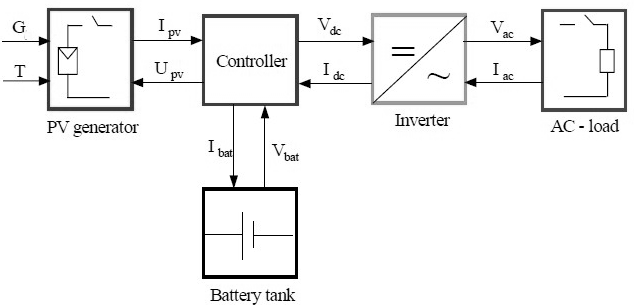
\includegraphics[width=0.95\textwidth]{blockdiagramPVS}
\centering
\caption{Block diagram for the stand-alone PV system. Source: \cite{Hansen}.}
\label{fig:blockdiagram}
\end{figure}

In the literature, there are several mathematical models available for each component of stand-alone PV systems. In this section, the mathematical model for each component of PV system is presented. 

%%%%%%%%%%%%%%%%%%%%%%%%%%%%%%%%%%%%%%%%%%%%%%%%%%%%%%%%
\subsubsection{PV generator (cell, module, string, and array) }
%%%%%%%%%%%%%%%%%%%%%%%%%%%%%%%%%%%%%%%%%%%%%%%%%%%%%%%%

A photovoltaic PV generator is the whole assembly of solar cells, connections, protective parts, and supports. In the present modeling, the focus is only on the cell/module/array.
 
The basic element of a PV System is the PV cell, also called a Solar Cell. A PV / Solar Cell is a semiconductor device that can convert solar energy into DC electricity. The semiconductor materials (usually silicon), which are specially treated to form an electric field, positive on one side (backside) and negative on the other (towards the sun). When solar energy (photons) hits the solar cell, electrons are knocked loose from the atoms in the semiconductor material, creating electron-hole pairs \cite{Lorenzo}. If electrical conductors are attached to the positive and negative sides, forming an electrical circuit, the electrons are captured in the form of electric current $ I_{ph} $ (photocurrent).
 
To increase their utility, a number of individual PV cells are interconnected together in a sealed, weatherproof package called Panel (or Module). For instance, a 12 V Panel will have 36 cells connected in series and a 24 V Panel will have 72 PV cells connected in series. In addition, to achieve the desired voltage and current, modules are wired in series (strings) and parallel into what is called a PV array, as shown in Fig.\ref{fig:celmodarray}. The flexibility of the modular PV system allows designers to create PV systems that can meet a wide variety of electrical demands. 

\begin{figure}[h]
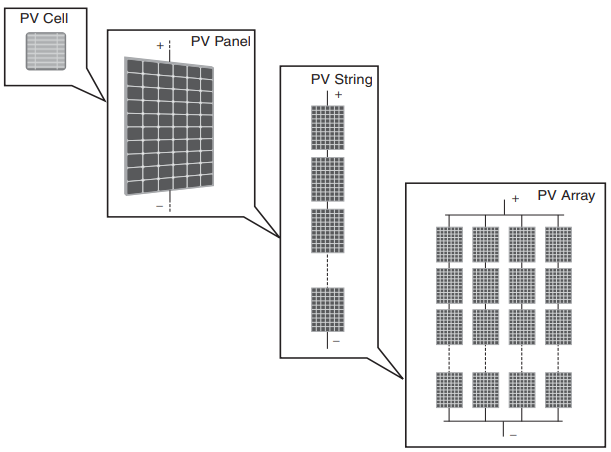
\includegraphics[width=0.95\textwidth]{PVarray}
\centering
\caption{PV cell, module, string and array. Source: \cite{SamlexSolar}.}
\label{fig:celmodarray}
\end{figure}

The PV modules are generally rated under standard test conditions (STC), which leads to the following specification by the manufacturers:  solar radiation of 1000 W/m$^{2}$, cell temperature of 25$^{o}$C, and solar spectrum of 1.5. The parameters required for the input of the PV modules are dependent on the meteorological conditions of the area to be serviced by photovoltaic solution. However, the climatic conditions are unpredictable due to the random nature of their occurrence \cite{Jakhrani}.
 
These uncertainties lead to either over- or underestimation of energy yield from PV modules. An overestimation of up to 40\% was reported as compared to the rated power output of PV modules \cite{Durisch}. The growing demand for photovoltaics technologies has led to research into the various aspects of its components from cell technology to the modeling, size optimization, and system performance \cite{Rajanna}, \cite{Badejani}; \cite{Yatimi}, \cite{Ferrari}, \cite{Saloux}, \cite{Hasan}, \cite{King}, \cite{Mellit}. Modeling PV modules is one of the major components responsible for proper functioning of PV systems. However, the estimation of models is affected by various intrinsic and extrinsic factors, which ultimately influence the behavior of current and voltage. Therefore, perfect modeling is essential to estimate the performance of PV modules in different environmental conditions \cite{Jakhrani}.
 
Modeling provides the means to understand the current, voltage, and power relationships of PV systems.
  
The performance of photovoltaic systems (solar cell/panels), that is, the output current/voltage curve ($I-V$ curve), is usually studied using an equivalent circuit model. This equivalent circuit consists of a current source with one or two diodes connected in parallel, and up to two resistors, one connected in parallel and the other one in series, to take into account energy losses in this model \cite{Cubas}. Based on these electronic components, four basic configurations are normally used when studying photovoltaic systems, as shown in Fig. \ref{fig:equivckt}. 

\begin{figure}[h]
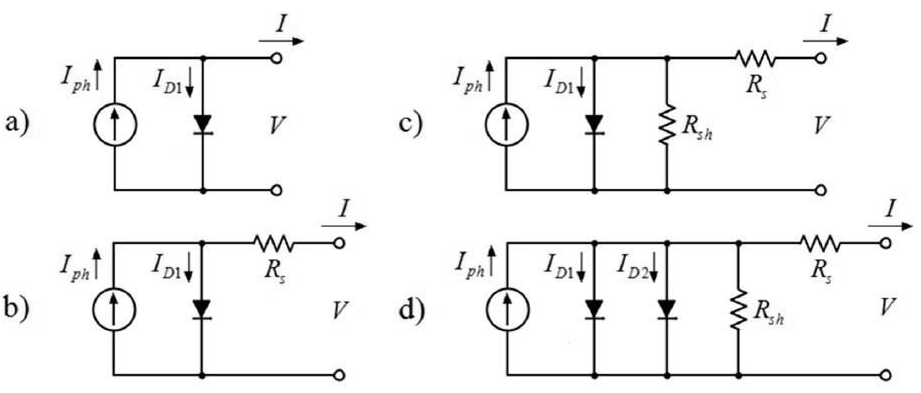
\includegraphics[width=0.95\textwidth]{equivckt}
\centering
\caption{Four different equivalent circuit models: (a) 1-diode; (b) 1-diode/1-resistor; (c) 1-diode/2-resistor; (d) 2-diode/2-resistor. Source: \cite{Cubas}.}
\label{fig:equivckt}
\end{figure}
 
The 1-diode model, whose equation to relate the output current, $I$, to the output voltage, $V$, is described in Equation \ref{eq:1diodemodel}. 

\begin{equation}
\label{eq:1diodemodel}
I = I_{ph}-I_{D1}=I_{ph}-I_{0}\left[ exp \left( \dfrac{V}{NaV_{T}} \right)  \right] 
\end{equation}

Where:
\begin{itemize}
\item $I_{ph}$ is the photocurrent delivered by the constant current source; 
\item $ I_{0} $ is the reverse saturation current corresponding to the diode; 
\item $ N $ is the number of series-connected cells in the photovoltaic system to be analyzed;
	\begin{itemize}
	\item $ N=1 $ in a single cell configuration. 	
	\end{itemize}	  
\item $ a $ is the ideality factor (or quality factor) that takes into account the deviation of the diodes from the Shockley diffusion theory; 
	\begin{itemize}
	\item $a=1$ for ideal diodes and between $ 1 $ and $ 2 $ for real diodes. 	
	\end{itemize}
\item $V_{T}$ is the thermal voltage ($ V_{T}=k_{B}T/q $);
	\begin{itemize}
	\item $ k_{B} $ is the Boltzmann constant ($ 1.3806503\times10^{-23}J/K $); 
	\item $ T $ is the temperature of the p-n junction (or cell temperature) expressed in Kelvin; 
	\item $ q $ is the absolute value of the electron's charge ($ -1.60217646\times10^{-19}C $).	
	\end{itemize}	 
\end{itemize}


This model has only three unknown parameters ($ I_{ph}$, $I_{0}$, and $a $), and it assumes that the series resistance is $ zero $ and shunt resistance is $ infinite $ and, thus, both of these parameters are ignored.
 
The 1-diode/1-resistor model, is described in Equation \ref{eq:1d1rmodel}. 

\begin{equation}
\label{eq:1d1rmodel}
I =I_{ph}-I_{0}\left[ exp \left( \dfrac{V+IR_{s}}{NaV_{T}} \right) -1 \right] 
\end{equation}

Where $R_{s}$ is the series resistor.

In this model, there are four unknown parameters ($ I_{ph}$, $I_{0}$, $ R_{s} $, and $ a $), and it assumes shunt resistance as $ infinite $.

The 1-diode/2-resistor model, is described in Equation \ref{eq:1d2rmodel}. 

\begin{equation}
\label{eq:1d2rmodel}
I =I_{ph}-I_{0}\left[ exp \left( \dfrac{V+IR_{s}}{NaV_{T}} \right) -1 \right] - \dfrac{V+IR_{s}}{R_{sh}}
\end{equation}

Where $R_{sh}$ is the shunt resistor.

In this model, there are five unknown parameters ($ I_{ph}$, $I_{0}$, $ R_{s} $, $ R_{sh} $, and $ a $).

And the 2-diode/2-resistor model, is described in Equation \ref{eq:2d2rmodel}. 

\begin{equation}
\label{eq:2d2rmodel}
I =I_{ph}-I_{01}\left[ exp \left( \dfrac{V+IR_{s}}{Na_{1}V_{T}} \right) -1 \right] - I_{02}\left[ exp \left( \dfrac{V+IR_{s}}{Na_{2}V_{T}} \right) -1 \right] - \dfrac{V+IR_{s}}{R_{sh}}
\end{equation}

This model has six unknown parameters with two exponential terms. 
Briefly, both single and double diode models require the knowledge of all unknown parameters, which is usually not provided by manufacturers. Nevertheless, the current-voltage equation is a transcendental expression \cite{Jakhrani}.  

However, regardless of the adopted model, the parameters of the equations must be estimated to adapt the corresponding model to the real behavior of the solar cell/panel. 

For this reason, researchers gradually focused on searching out the approximate methods for the calculation of unknown parameters, proceeding along three different paths. The analytical methods give exact solutions by means of algebraic equations, as done by \cite{Cubas} and \cite{Brano}. However, due to the implicit nature and nonlinearity of PV cell or module characteristics, it is hard to discover the analytical solution of all unknown parameters, as described in \cite{Hasan}. Thus, numerical methods such as the Newton-Raphson method or the Levenberg-Marquardt algorithm were preferred, as described by \cite{Mellit}. This happens because numerical methods give approximate solutions to the nonlinear problems without searching for exact solutions. However, numerical methods are time consuming and need long term time series data, which is not available in developing countries. \cite{Jakhrani} used mixed methodology bringing analytical and numerical steps together.  \cite{Shenawy} create a method to discover the unknown parameters of the PV panels through experimentation (essays). And \cite{Tian} used a mix of analytical and experimental methodology to establish the unknown parameters, but samples of the PV modules are necessary to perform some essays, when we use the experimental technique. 

Therefore, a wide variety of models exists for estimation of the power output of PV modules (and $I-V$ or $P-V$ curves). However, this study will rely on the simplified 1-diode model, that was shown by \cite{Saloux} that has a small error rate, between 0.03\% and 4.68\% from selected PV panels tested. In addition, this mathematical modeling has the advantage of being an explicit model, which does not use iterative numerical calculation. 

%%%%%%%%%%%%%%%%%%%%%%%%%%%%%%%%%%%%%%%%%%%%%%%%%%%%%%%%
\subsubsection{The Proposed PV Panel Model}
%%%%%%%%%%%%%%%%%%%%%%%%%%%%%%%%%%%%%%%%%%%%%%%%%%%%%%%%

With the proposed model, an explicit set of equations is derived from the ideal PV model given by Equation~\ref{eq:1diodemodel}.

A single-diode without series and shunt resistances is considered. Equation~\ref{eq:1diodemodel} is used to write down expressions for currents and voltages at each key point shown in Fig. \ref{fig:ivcurve}.

\begin{figure}[h]
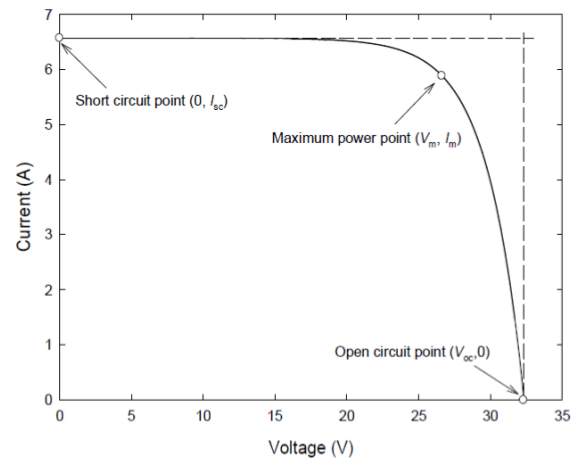
\includegraphics[width=0.7\textwidth]{ivcurve}
\centering
\caption{$ I-V $ characteristic curve of an ideal PV cell. Source: \cite{Saloux}.}
\label{fig:ivcurve}
\end{figure}

Hence, the short-circuit current, the open-circuit voltage, the maximum power voltage and current are written as defined by \cite{Saloux} and shown in Equations \ref{eq:Isc} to \ref{eq:Im}.

\begin{equation}
\label{eq:Isc}
I_{sc}=I_{ph}\vert_{V=0}
\end{equation}

\begin{equation}
\label{eq:Voc}
V_{oc}=\dfrac{aNk_{B}T}{q}ln\left( 1+\dfrac{I_{sc}}{I_{0}} \right) 
\end{equation}

\begin{equation}
\label{eq:exp}
exp\left( \dfrac{qV_{oc}}{aNk_{B}T} \right) = \left(1+\dfrac{qV_{m}}{aNk_{B}T} \right) exp \left( \dfrac{qV_{m}}{aNk_{B}T} \right) 
\end{equation}

\begin{equation}
\label{eq:Im}
I_{m} =I_{ph}-I_{0}\left[ exp \left( \dfrac{qV_{m}}{aNk_{B}T} \right) -1 \right] 
\end{equation}

Equation \ref{eq:exp} is not explicit with regard to the key PV  parameters, it therefore needs to be rewritten in a different way. A PV cell has a hybrid behavior, i.e., a current-source at the short-circuit point and a voltage-source at the open-circuit point \cite{Saloux}. These two regions are characterized by two asymptotes of the $ I-V $ curve in Fig. \ref{fig:ivcurve}, where the transition is a compromise between both behaviors. It is interesting to observe that the maximum power point corresponds to a trade-off condition, where the current is still high enough before it starts decreasing with the increase in the output voltage (Fig. \ref{fig:ivcurve}).

Based on this, the tangent of the I-V curve can be used to evaluate the transition between current- to voltage-source controlled regions; this operation yields Equation \ref{eq:didv}.

\begin{equation}
\label{eq:didv}
\dfrac{dI}{dV}=-\dfrac{qI_{0}}{aNk_{B}T}exp \left( \dfrac{qV}{aNk_{B}T}  \right) 
\end{equation}

The derivative of Equation \ref{eq:didv} is used to calculate the output voltage that corresponds to the maximum power operation condition of the cell, thus generating the Equation \ref{eq:Vmderiv}.

\begin{equation}
\label{eq:Vmderiv}
V_{m}=\dfrac{aNk_{B}T}{q} ln \left( -\dfrac{qNk_{B}T}{qI_{0}} \left( \dfrac{dI}{dV}  \right)_{V_{m}}   \right) 
\end{equation}

It is evident that Equation \ref{eq:Vmderiv} requires an expression of the derivative of the current with voltage evaluated at the maximum power point. The fact that the maximum power corresponds to an extreme, the variation of the maximum output power with voltage is relatively small, i.e., a change in $ V_{m} $ has a relatively small effect on the maximum power of the cell \cite{Saloux}. Consequently, considering the asymptotic behavior of the $I-V$ curve in short- and open-circuit conditions, the derivative required by Equation 10 can be calculated as shown in Equation \ref{eq:dIdV_Vm}.

\begin{equation}
\label{eq:dIdV_Vm}
\dfrac{dI}{dV}\vert_{V_{m}} \cong -\dfrac{0-I_{sc}}{V_{oc}-0}=\dfrac{I_{sc}}{V_{oc}}
\end{equation}

Replacing the Equation \ref{eq:dIdV_Vm} into Equations \ref{eq:Vmderiv} and \ref{eq:Im}, the voltage and the current at the maximum power point and consequently the maximum output power, are expressed by Equations \ref{eq:Vmfinal}, \ref{eq:Imfinal}, and \ref{eq:Pm} ($ P_{m}=V_{m}I_{m} $). These equations are used to calculate the key cell parameters at the maximum power point (MPPT) as a function of cell temperature and parameters from the manufacturer's data-sheet.

\begin{equation}
\label{eq:Vmfinal}
V_{m}=\dfrac{aNk_{B}T}{q} ln \left( \dfrac{aNk_{B}T}{qI_{0}} \dfrac{I_{sc}}{V_{oc}}  \right) 
\end{equation}

\begin{equation}
\label{eq:Imfinal}
I_{m} = I_{ph} + I_{0} - \dfrac{aNk_{B}T}{q} \left( \dfrac{I_{sc}}{V_{oc}} \right)  
\end{equation}

\begin{equation}
\label{eq:Pm}
P_{m} = \left[ \dfrac{aNk_{B}T}{q} ln \left( \dfrac{aNk_{B}T}{qI_{0}} \dfrac{I_{sc}}{V_{oc}}  \right) \right] \times \left[ I_{ph} + I_{0} - \dfrac{aNk_{B}T}{q} \left( \dfrac{I_{sc}}{V_{oc}} \right)  \right] 
\end{equation}


However, the photocurrent delivered by the constant current source ($ I_{ph} $) or even the reverse saturation current ($ I_{0} $) is not given by PV manufacturers. Therefore, Equation \ref{eq:Iph} is used to calculate the photocurrent as a function of irradiance and temperature \cite{Villalva}.

\begin{equation}
\label{eq:Iph}
I_{ph}=\dfrac{G}{G_{ref}} \left[ I_{ph,ref} + \mu_{I} \left( T-T_{ref} \right)    \right] 
\end{equation}

\noindent where the reference state (STC) of the cell is given by the solar irradiance $ G_{ref}=1000 W/m^{2} $, and the temperature $ T_{ref}=298.15 K (=25^{o}C) $.

In Equation \ref{eq:Iph}, $ \mu_{I} $ is the short-circuit current temperature coefficient ($A/K$) and corresponds to the photocurrent obtained from a given PV cell working at (STC or standard test conditions) reference conditions (provided by PV manufacturers). $ I_{ph,ref} $ can also be approximated to the reference short-circuit current that is provided by PV manufacturers ($ I_{sc,ref} $) as shown by \cite{Jakhrani}.

The cell temperature ($ T $) can be obtained from \cite{Ross} and is shown in Equation \ref{eq:Tcell}.

\begin{equation}
\label{eq:Tcell}
T = T_{air} + \dfrac{NOCT-20}{800}G
\end{equation}

\noindent where $ T_{air} $ is the ambient temperature, $NOCT$ is the nominal operating cell temperature (in $^{o}$C) that is found on the PV manufacturer's data-sheet, and $G$ is the solar irradiance ($ W/m^{2} $) at the location of the PV system.

Furthermore, \cite{Villalva} have proposed a relationship, which allows the saturation current ($ I_{0} $) to be expressed as a function of the cell temperature. In this study, this relation is explicitly written based on cell open-circuit conditions using the short-circuit current temperature coefficient in addition to the open-circuit voltage temperature coefficient (Equation \ref{eq:I0}).

\begin{equation}
\label{eq:I0}
I_{0} = \dfrac{I_{sc,ref} + \mu_{I}(T - T_{ref})}{exp \left[ \dfrac{q(V_{oc,ref} + \mu_{V} (T - T_{ref}))}{aNk_{B}T}    \right] -1}
\end{equation}

\noindent where $ V_{oc,ref} $ is the reference open-circuit voltage, and $ \mu_{V} $ is an open-circuit voltage temperature coefficient ($ V/K $).

The ideality (or quality) factor of the diode $ a $, which is usually considered as a constant \cite{Villalva}, is determined in the reference state. Using the maximum power point current equation (Equation \ref{eq:Pm}) and the saturation current in the reference temperature given by Equation \ref{eq:I0}, the diode quality coefficient is determined by Equation \ref{eq:a}.

\begin{equation}
\label{eq:a}
a = \dfrac{q(V_{m,ref}-V_{oc,ref})}{Nk_{B}T} \dfrac{1}{ln \left( 1 - \dfrac{I_{m,ref}}{I_{sc,ref}}  \right) }
\end{equation}

\noindent where $ V_{mref} $, $ V_{oc,ref} $, $ I_{m,ref} $, and $ I_{sc,ref} $ are key cell values obtained under both actual cell temperature and solar irradiance conditions, usually provided by the manufacturers.

The model is now completely determined, i.e., with all the variables defined. This model requires the actual cell temperature (or the air temperature), the actual solar irradiance and common data provided by manufacturers.

If the PV cells are in parallel, then there is a parallel array. There will therefore be a change in the $ I_{ph} $ and $ I_{0} $and the resulting current is given by Equation \ref{eq:Iarray}, as demonstrated in \cite{Saloux}.

\begin{equation}
\label{eq:Iarray}
I_{array} = (N_{cells in parallel})(I_{one cell})
\end{equation}

\noindent where $ I_{one cell} $ is the current from Equation \ref{eq:Imfinal}.

In addition, if the panels are in series, the current does not change but the total voltage is the sum of the voltage of each individual panel.

\begin{equation}
\label{eq:Varray}
V_{array} = (N_{cells in series})(V_{one panel})
\end{equation}

\noindent where $ V_{one panel} $ is the voltage from Equation \ref{eq:Vmfinal}.

%%%%%%%%%%%%%%%%%%%%%%%%%%%%%%%%%%%%%%%%%%%%%%%%%%%%%%%%
\subsubsection{Battery Storage Model }
%%%%%%%%%%%%%%%%%%%%%%%%%%%%%%%%%%%%%%%%%%%%%%%%%%%%%%%%

Because of the fluctuating nature of the output delivered by the PV arrays, batteries are an essential part of a PV system. Thus, during the hours of sunshine, the PV system feeds the load directly and excess electrical energy is stored in the battery. During the night, or during a period with low solar irradiation, energy is supplied to the load from the battery \cite{Mellit}.
  
Several models have been presented in the literature. However, regardless of the model, normally the following parameters are normally required: 

\begin{itemize}
\item Nominal capacity ($ q_{m} $), is the number of Ampere-hours ($ Ah $) that can maximally be extracted from the battery, under predetermined discharge conditions.
\item State of charge ($ SOC $), is the ratio between the present capacity and the nominal capacity, i.e., $ SOC = q/q_{max} $. Obviously $ 0<SOC<1 $. If $ SOC=1 $, then the battery is totally charged; and if $ SOC=0 $, the battery is fully discharged
\item Charge (or discharge) regime.This parameter reflects the relationship between the nominal capacity of a battery and the current at which it is charged (or discharged). It is expressed in hours: for instance, discharge regime is 30h for a battery of 150 Ah that is discharged at 5A.
\item Efficiency ($\eta_{b}$), is the ratio of the charge extracted during discharge divided by the amount of the charge needed to restore the initial state of charging or discharging current. 
\item Lifetime, is the number of charge/discharge cycles the battery can sustain before losing 20\% of its nominal capacity.
\end{itemize}

The merit of a stand-alone PV system is evaluated in terms of the reliability of the electricity supply to the load and in terms of the long-term efficiency of the components. Battery efficiency was described in this section, and the liability is quantified by the concept of loss of load probability (LLP). LLP is defined as the ratio between the Ampere-hour deficit and the Ampere-hour demand, both with respect to the load, over a long period of time \cite{Copetti}. 

In general, the battery models view the battery as a voltage source $ E $ in series with an internal resistance $ R_{0} $, as shown in Fig. \ref{fig:batteryckt}. 

\begin{figure}[h]
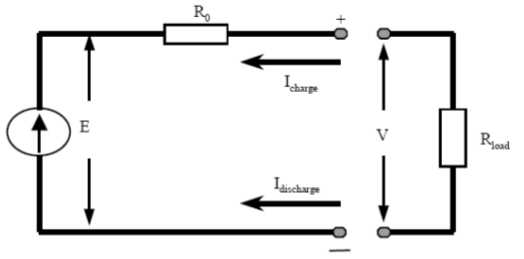
\includegraphics[width=0.5\textwidth]{batteryckt}
\centering
\caption{Schematic diagram of the battery. Source: \cite{Hansen}.}
\label{fig:batteryckt}
\end{figure}

The terminal voltage of the battery can be expressed in terms of its open circuit voltage and the voltage across the internal resistance of the battery \cite{Sukamongkol}, as shown by Equation 31.  

Where $ V_{b} $ is the battery terminal voltage, $ E_{oc} $ is the battery circuit voltage, $ I_{b} $ is the battery current, and $ R_{b} $ is the internal resistance of the battery.

The battery model, which describes the relationship between the voltage, the current and the state of charge, can be found in \cite{Copetti}, \cite{Manwell93}, and \cite{Manwell94}.  

Manwell and McGowen's Kinetic Battery Model (KiBaM)  \cite{Manwell93} was developed at the University of Massachusetts to predict the performance of the battery, based on manufacturer's data. However, it uses some data extracted from batteries tested in laboratory. It is therefore not suitable for this study. 

Most of the models created were used to simulate and optimize PV storage systems based on lead-acid batteries, the most commonly used batteries in PV applications, owing to their relative low cost and wide availability \cite{Copetti}. 

Here, the model adopted is the based on \cite{Copetti}, who uses manufacturer's data and allows finding relations among voltage, current, state of charge and temperature. 

The discharge voltage equation is shown in Equation \ref{eq:bat_Vd}. The first term represents the voltage variation with the state of charge ($ SOC $), i.e., the electrolyte concentration, and the second is the variation due to internal resistance variation.

\begin{equation}
\label{eq:bat_Vd}
V_{d} = \left[ 2.085-0.12(1-SOC) \right] - \dfrac{I}{C_{10}} \left( \dfrac{4}{1+I^{1.3}} + \dfrac{0.27}{SOC^{1.5}}+0.02 \right) (1-0.007 \Delta T)
\end{equation}

\noindent where $ C_{10} $ means 10h of rated capacity, which is standard on the manufacturer's data-sheet, $ \Delta T $ is temperature variation ($ \Delta T=T-T_{ref} $, $ T_{ref}=25^{o}C $, $ SOC $ indicates how much electric charge is stored in the cell at any given time, defined by Equation \ref{eq:SOCbat}.

\begin{equation}
\label{eq:SOCbat}
SOC = \left( 1 - \dfrac{Q}{C} \right) 
\end{equation}

\noindent where $ Q $ is the charge delivered at the time of interest ($ Q=It $), and C is the battery capacity.

The ratio between $ Q $ and $ C $ represents the depth of discharge ($ DOD $) or the fraction of discharge, i.e., $ DOC=1-SOC $.

The efficiency of the battery discharge is assumed to be 100\%, according to \cite{Copetti}; however, the total amount of useful charge available during discharge is limited by the current rate and temperature given by Equation \ref{eq:CC10}. This equation, known as capacity, is normalized with respect to discharge current corresponding to $ C_{10} $ rated capacity ($ I_{10} $).

\begin{equation}
\label{eq:CC10}
\dfrac{C}{C_{10}} = \dfrac{1.67}{1+0.67 \left( \dfrac{I}{I_{10}} \right)^{0.9} }(1+0.005 \Delta T)
\end{equation}

Note that when the discharge current tends to zero at 25$^{o}$C, the maximum capacity that can be removed is about 67\% over the capacity.

For the charging process, however, the parameters are presented in Equation \ref{eq:Vcbat}.

\begin{equation}
\label{eq:Vcbat}
V_{c} = [2+0.16SOC]+ \dfrac{I}{C_{10}} \left( \dfrac{6}{1+I^{0.86}} + \dfrac{0.48}{(1-SOC)^{1.2}} + 0.036  \right) (1-0.025 \Delta T)
\end{equation}

SOC can be calculated easily at any point during the discharge period; however, during recharge it is much more difficult \cite{Copetti}.

Generally, the efficient region is where $ SOC $ is below $ 0.7 $ and $ V_{c} $ is less than $2.3 V$ per cell. The efficiency drops to zero at full charge and the function that represents the charge efficiency ($ \eta_{c} $) variation with state of charge and current rate is given in Equation \ref{eq:efficcharge}.

\begin{equation}
\label{eq:efficcharge}
\eta_{c} = 1 - exp \left[ \dfrac{20.73}{\dfrac{I}{I_{10}}+0.55} (SOC-1) \right] 
\end{equation}

\cite{Copetti} show that, during overcharge, gassing occurs and tests have demonstrated that the final charge voltage ($ V_{ec} $) increases with the current intensity and with the decrease in temperature (Equation \ref{eq:Vec}). A function was created for the gassing voltage also, as shown in Equation \ref{eq:Vg}. In addition, the overcharge phenomenon can be represented by Equation \ref{eq:Voverc}.

\begin{equation}
\label{eq:Vec}
V_{ec} = \left[ 2.45 + 2.011 ln \left( 1+\dfrac{I}{C_{10}} \right)  \right] (1-0.002 \Delta T)
\end{equation}

\begin{equation}
\label{eq:Vg}
V_{g} = \left[ 2.24 + 1.97 ln \left( 1+\dfrac{I}{C_{10}} \right)  \right] (1-0.002 \Delta T)
\end{equation}

\begin{equation}
\label{eq:Voverc}
V_{c} = V_{g} + (V_{ec} - V_{g}) \left[ 1- exp \left( \dfrac{Ah_{restored}-0.95C}{I\tau}  \right)    \right] 
\end{equation}

\noindent where $ Ah_{restored} $ represents the Ampere-hour stored in the battery with regard to the battery capacity ($ C $) during this hour.

The function assumes that 95\% of the capacity has already been restored at the start of overcharge.

The time constant of the phenomenon ($ \tau $) is inversely proportional to the charge intensity and can be written as Equation \ref{eq:tau}.

\begin{equation}
\label{eq:tau}
\tau = \dfrac{17.3}{1+852 \left( \dfrac{I}{C_{10}} \right) ^{1.67} }
\end{equation}

Equation \ref{eq:Vcbat} can therefore be used to model the voltage ($ V_{c} $) evolution of the battery, at the start of gassing ($ V_{c} \leq V_{g} $). During overcharging ($ V_{c} > V_{g} $), Equation \ref{eq:Voverc} can be used until a constant final voltage ($ V_{ec} $) is reached.

The battery's storage capacity can be calculated using Equation \ref{eq:stor}, as defined in \cite{Wenham}.

\begin{equation}
\label{eq:stor}
Storage capacity = \dfrac{N_{C}E_{load}}{DOD \eta _{b}}
\end{equation}

\noindent where $ DOD $ is the maximum possible depth of battery discharge, $ E_{load} $ is the average energy consumed by the load, $ N_{C} $ is the largest number of continuous cloudy days of the area, and $ \eta_{b} $ is the efficiency of the battery.

As an example of this formula's application, as shown in \cite{Abdulateef}, considering that an off-grid PV system is intended to supply $1.5 kW/48 V$ for 24 hours ($=36 kWh$); The largest number of continuous cloudy days in the selected site is about 1 day; For a maximum depth of battery discharge $DOD$ of $0.8$ and battery efficiency at $80\%$.

Using Equation \ref{eq:stor}, the storage capacity then becomes $56.3 kWh$. Since the selected DC bus voltage is $48 V$, then the required Ampere-hours of the battery is $1173 Ah$ ($56.3 kWh/48$). If a single battery is 12 V and 350 Ah, then four batteries are connected in series ($4 \times 350 Ah = 1400 Ah$).

In this study, a simplified model for battery charging (Equation \ref{eq:charge}) and discharging (Equation \ref{eq:discharge}) was considered, even recognizing that the process is not linear and is temperature-dependent. The equations are used to update the $SOC$ of the batteries, and have the number of hours ($ Num_{h} $) as a variable. There is a factor (1.15) which is present in the charging equation, and is necessary to express that during the charging process it is usual to reach 115\% of the battery capacity.

\begin{equation}
\label{eq:charge}
SOC_{charge} = SOC_{previous} + \dfrac{100*Pm*Num_{h}}{V_{system}*capacity*N_{BP}*1.15}
\end{equation}

\begin{equation}
\label{eq:discharge}
SOC_{discharge} = SOC_{previous} - \dfrac{100*I_{drained}*Num_{h}}{capacity}
\end{equation}

It is worth mentioning that, specifically for PV systems used in Brazil, a Regulation (RN 493/2012), issued by the Brazilian Electricity Regulatory Agency (Aneel) establishes a minimum of 48 hours of battery autonomy for stand-alone solar PV systems, among others related definitions.

%%%%%%%%%%%%%%%%%%%%%%%%%%%%%%%%%%%%%%%%%%%%%%%%%%%%%%%%
\subsubsection{Controller Model}
\label{sec:controller}
%%%%%%%%%%%%%%%%%%%%%%%%%%%%%%%%%%%%%%%%%%%%%%%%%%%%%%%%

Depending on the literature, the controller can receive different names: controller \cite{Hansen}, charge controller \cite{Mahanta} and \cite{Chauhan}, regulator \cite{Mellit}, DC-DC converter with MPPT and switch \cite{Dhanowa}, \cite{Yatimi}, \cite{Abdulateef}, \cite{Roy}. However, in this study, in order to simplify, the term used is controller. 

The controller is a set of items (DC-DC converter, a MPPT and switches) and can be defined as the responsible to manage the energy flow to PV system, batteries and loads by collecting information on the battery voltage and knowing the maximum and minimum values acceptable for the battery voltage. According to \cite{Pinho}, controllers aim to protect the battery (or batteries) against the excessive charge and discharge, improving its lifetime. 

Controllers with MPPT mechanism are the mostly used nowadays,  and it maintains the PV operating at the stage of maximum power.

As defined by \cite{Hansen} and \cite{Mellit}, all power systems must include a control strategy, which describes the interactions between its components. The use of battery as a storage form implies thus the presence of a charge controller. 

In general, there are two main operating modes for the controller: normal operating condition, when the battery voltage fluctuates between maximum and minimum voltages; and overcharge or over-discharge conditions, which occur when the battery voltage reaches some critical values. 

In \cite{Mellit} was established that the controller allows the management of energy between the load and the battery. The input signals for regulator model are the battery current ($ I_{br} $), PV generator's voltage ($ V_{PV} $), PV generator's current ($ I_{PV} $), and battery voltage ($ V_{b} $). The outputs are battery ($ I_{rb} $) current and used current ($ I_{u} $). 

According \cite{Hansen}, to protect the battery against an excessive charge, the PV arrays are disconnected from the system, when the terminal voltage increases above a certain threshold $ V_{max \textunderscore off} $ and when the current required by the load is less than the current delivered by the PV arrays. PV arrays are connected again when the terminal voltage decreases below a certain value $ V_{max \textunderscore on} $. This can be done by using a switch with a hysteresis cycle, as illustrated in Fig. \ref{fig:controllerover}. 

\begin{figure}[h]
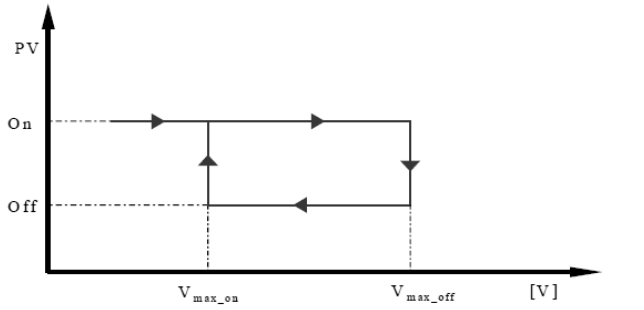
\includegraphics[width=0.7\textwidth]{controllerover}
\centering
\caption{Operating principle of an overcharge protector. Source: \cite{Hansen}.}
\label{fig:controllerover}
\end{figure}

To protect the battery against excessive discharge, the load is disconnected when the terminal voltage falls below a certain threshold i and when the current required by the load is larger than the current delivered by the PV arrays \cite{Hansen}. The load is reconnected to the system, when the terminal voltage is above a certain value i, using a switch with a hysteresis cycle, as shown in Fig. \ref{fig:controllerdisc}. 

\begin{figure}[h]
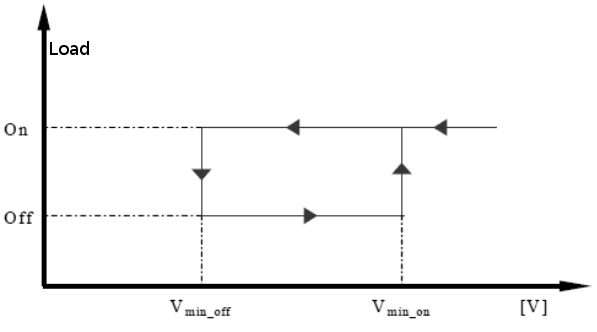
\includegraphics[width=0.7\textwidth]{controllerdisc}
\centering
\caption{Operating principle of a discharge protector. Source: \cite{Hansen}.}
\label{fig:controllerdisc}
\end{figure}

According to \cite{Lorenzo}, the switches may either be electromechanical (relay, contactors, etc.) or solid state (bipolar transistors, MOSFET's, etc.). 

The steps in the modeling of the controller process are summarized in Table \ref{table:controller}.

\begin{table}[!t]
%% increase table row spacing, adjust to taste
\renewcommand{\arraystretch}{1.3}
% if using array.sty, it might be a good idea to tweak the value of
% \extrarowheight as needed to properly center the text within the cells
\caption{Summary of the controller process. Source: adapted from~\cite{Hansen}}
\label{table:controller}
\centering
%% Some packages, such as MDW tools, offer better commands for making tables
%% than the plain LaTeX2e tabular which is used here.
\begin{tabular}{c | c | c }
\hline
\hline
Step  & Constraint & Command\\
\hline
\hline
(1) & \makecell{If $V > V_{max \_ off}$ \\and $I_{load} < I_{pv}$} & \makecell{Disconnect PV array \\from the system}\\
\hline
(2) & \makecell{If command (1) is \\done and $V < V_{max \_ on}$} & \makecell{Reconnect PV array \\to the system}\\
\hline
(3) & \makecell{If $V < V_{min \_ off}$ and \\ $I_{load} > I_{pv}$} & \makecell{Disconnect the load \\from the system}\\
\hline
(4) & \makecell{If command (3) is \\ done and $V > V_{min \_ on}$} & \makecell{Reconnect the load \\to the system}\\
\hline
\hline
\end{tabular}
\end{table}

Regarding the DC-DC converter, the most basic idea is that the power is converted while altering the current and voltage. 

As shown in \cite{Abdulateef}, the DC-DC converter is used to increase the efficiency of the PV system by matching the voltage generated by PV array to the voltage required by the load. The output power ($ P_{out} $) of DC-DC converter is given by Equation \ref{eq:poutcont}. 

\begin{equation}
\label{eq:poutcont}
P_{in} = P_{out}
\end{equation}

Assuming that the efficiency of the controller ($ \eta_{c} $) is a manufacturer's data, from Equation \ref{eq:poutcont} is possible to reach Equation \ref{eq:potcont}.

\begin{equation}
\label{eq:potcont}
V_{in} I_{in} \eta_{c} = V_{out} I_{out}
\end{equation}

Where $ V_{in} $ is the voltage across the PV array, $ I_{in} $ is the current output of PV array, $ V_{out}$ is the  DC bus voltage, and $I_{out}$ is the output current from the converter, when all the other values are known.

Worth to mention that $ V_{out}$, depending on the PV panel generation and on the batteries charge, it can be the voltage that charges the battery $V_{b}$ (which is bigger than the nominal voltage of the batteries), the voltage that is feed by the batteries (the same $V_{b}$ but with levels that can be lower than it, or even the voltage that comes from the PV panels and depends on the MPPT system employed by the controller.

The output voltage is related to the input voltage as a function of duty cycle of the switch (\cite{Abdulateef}). 
 
A DC-DC converter can either be step-up (Boost), step-down (Buck), or both increase and decrease (Buck-Boost) the voltage, as defined by \cite{Mahanta}. In addition, there is the Cuk converter, which is a Buck-Boost converter with an inverting topology \cite{Catherine}. 

For the Cuk converter, the relationship is expressed by \ref{eq:voutvin} as show in \cite{Abdulateef}.

\begin{equation}
\label{eq:voutvin}
\dfrac{V_{out}}{V_{in}} = \dfrac{D}{D-1}
\end{equation}

Where $D$ is the duty cycle or ratio of the circuit converter, i.e., it is defined as the ratio of the on time of the switch to the total switching period.
 
The DC/DC converter should always operate in the MPPT to maximize the PV array efficiency and consequently increase the efficiency of the PV system, as defined in \cite{Yatimi}.
  
Various types of MPPT schemes are proposed by researchers, namely open circuit, short circuit, perturb and observe (P\& O)/hill climbing, incremental conductance, and so forth, as shown by \cite{Haque}.
 
As the MPPT definition and the equations to get the maximum power from the PV panels was described at the end of the PV panel modeling, the important here is to notice that the Equation \ref{eq:voutvin} defines the relationship between the input signal, the efficiency of the controller and the output power.
 
\subsubsection{The inverter model}
As shown by \cite{Mellit}, the PV arrays produce DC and therefore when the PV system contains an AC load, a DC/AC conversion is required. An inverter is a converter, where the power flows from DC to AC side, i.e., having a DC voltage as input; it produces AC voltage, as output. The role of the inverter is to keep the voltage constant on the AC side, i.e., at the rated voltage (127 V or 220 V, for example), and to convert the input power $ P_{in} $ into the output power $ P_{out} $ with the best possible efficiency \cite{Hansen}.

The inverter is characterized by a power dependent efficiency $ \eta_{i} $ given by \cite{Hansen} as shown by Equation \ref{eq:efficinv}.

\begin{equation}
\label{eq:efficinv}
\eta_{i} = \dfrac{P_{out}}{P_{in}} = \dfrac{V_{AC} I_{AC} cos\varphi}{V_{DC}I_{DC}}
\end{equation}

Where $ I_{DC} $ is the current required by the inverter from the DC source in order to be able to keep the rated voltage on the AC side, $ V_{DC} $ is the input voltage to the inverter delivered by the DC source (PV panel or battery),  $ V_{AC}  $ and $ I_{AC} $ are the output voltage and current, respectively, and $ cos \varphi $ can be found from the inverter's data-sheet.

Therefore, with this equation it is possible to simulate the output power of the inverter, based on information from the inverter's data-sheet and from the DC module or the PV panel that feed the inverter (which are obtained by this study model).

%--------------------------------------------------
\subsection{Availability of Stand-alone PV Systems}
\label{sec:availability}
%--------------------------------------------------

Each stand-alone PV system, like any other power systems, has a specific level of availability. This reliability level impacts various issues, as system performance, production, feasibility, and investment. 

The availability of a stand-alone PV system can be defined as the percentage of time at which a power system is capable of meeting the load requirements~\cite{Khatib2014}. The number of hours that the system is available, divided by 8,760 h, gives the annual system availability.
The system availability definition depends on how critical the load application is. For critical loads, 99\% is considered acceptable. While in a ordinary house electrical load, 95\% is considered acceptable. 

As an example, a system with 95\% availability is expected to meet the load requirement of 8,322 h during an average year for the entire useful life of the system. An annual availability of 99\% means that the system can operate the load for 8,672 h of the 8,760 h.

With that in mind, it is important to mention that even if a formal verification or a simulation shows that a PV system fails, it doesn't mean that the sizing is wrong. It is important to evaluate how critical the load application is and the horizon of evaluation. However this analysis can be useful, for example, to improve the sized battery autonomy.

%%%%%%%%%%%%%%%%%%%%%%%%%%%%%%%%%%%%%%%%%%%%%%%%%%%%%%%%
\subsection{Sizing Stand-alone Solar Photovoltaic Systems}
%%%%%%%%%%%%%%%%%%%%%%%%%%%%%%%%%%%%%%%%%%%%%%%%%%%%%%%%

The mathematical model presented at section~\ref{model} is important for the project validation, however if it is included an approach to perform the sizing of stand-alone PV systems, than the proposed tools at this Thesis can perform the system validation (the intended behavior), and moreover to obtain the optimal project sizing.

The sizing check stage can ensure that the system meets the standard project steps related 
to critical period solar energy method~\cite{Pinho} and adopting MPPT (Maximum Power Point Tracking) charge controller,
which is the most common one in practice. Firstly, we need to correct the energy consumption estimated to the load 
($E_{consumption}$), which is carried out by Eq.~\eqref{eq:Ecorrected}, where the efficiency of batteries ($\eta_{b}$), 
controller ($\eta_{c}$), and inverter ($\eta_{i}$) are considered~\cite{Pinho} as follows
%
\begin{equation}
\label{eq:Ecorrected}
E_{corrected} = \dfrac{E_{consumption}}{\eta_{b} \eta_{c} \eta_{i} }.
\end{equation}

We also need to estimate the energy that can be produced for each panel, called $E_{p}$, in Wh, defined as
%
\begin{equation}
\label{eq:Ep}
E_{p} = Solar\_Irradiance \times Panel\_Area \times \eta_{p} \times 1000,
\end{equation}

\noindent where the solar irradiance is expressed in terms of $kWh/m^{2}$ and depends on the site where the PV system will be deployed; 
the PV panel area is given in $m^{2}$ and corresponds to the size of one PV panel, and $\eta_{p}$ represents the PV panel efficiency.
The total minimum number of needed solar panels ($N_{TPmin}$) is computed as
%
\begin{equation}
\label{eq:NTPmin}
N_{TPmin} = \dfrac{E_{corrected}}{E_{p}}.
\end{equation}

Particularly, the total number of panels in series ($N_{PSmin}$) and parallel ($N_{PPmin}$) are respectively given by
%
\begin{equation}
\label{eq:NPSmin}
\dfrac{V_{mppt,min}}{V_{maxPower,TempMax}} \leq N_{PSmin} \leq \dfrac{V_{mppt,max}}{V_{maxPower,TempMin}},
\end{equation}
%
\begin{equation}
\label{eq:NPPmin}
N_{PPmin} = \dfrac{P_{total}}{Number\,Panels\,Series \times P_{max,ref}},
\end{equation}
%
\noindent where $V_{mppt,max}$ is the maximum operation voltage and $V_{mppt,min}$ 
is the minimum operation voltage of the charge controller; $V_{maxPower,TempMax}$ and 
$V_{maxPower,TempMin}$ are the maximum power voltage from the PV module considering 
the maximum and minimum operational temperature, respectively; 
$P_{total}$ is the total power demanded from the PV system and 
$P_{max,ref}$ is the power supplied from one PV panel in $Watts$.
Regarding batteries, we must first define the total capacity of the battery bank, which can be described as
%
\begin{equation}
\label{eq:Cbank}
C_{bank} = \dfrac{E_{corrected} \times autonomy}{V_{system} \times DOD},
\end{equation}

\noindent where the variable $autonomy$ is a design definition and normally has a value ranging from $6$ to $48$h; 
$ V_{system} $ is the DC voltage of the bus, and $ DOD $ is the battery deep of discharge (considered of maximum of 25\% here).
%
Secondly, the total number of batteries is computed as 

\begin{equation}
\label{eq:Nbtotal}
N_{B}total = N_{BS}min \times N_{BP}min = \dfrac{V_{system}}{V_{bat}} \times \dfrac{C_{bank}}{1 \,Battery \, Capacity}.
\end{equation}

Moreover, the Equation \ref{eq:batcheck} perform the final sizing check, considering the number of batteries in series ($ N_{BS} $) and the number of batteries in parallel ($ N_{BP} $) adopted by the project.

\begin{equation}
\label{eq:batcheck}
\left( N_{BS} \times  N_{BP} \right) \geq N_{B}total
\end{equation}

Regarding the charge controller, it must initially meet the voltage requirement of the PV system, as described by Eq.~\eqref{eq:vcvsystem} to the charge controller voltage: 
\begin{equation}
\label{eq:vcvsystem}
V_{c} = V_{system}.
\end{equation}

The short circuit reference information from the manufacturer's solar panel must be corrected 
to the cell temperature because the field temperature is higher than the nominal or laboratory temperature, 
and PV system is temperature dependent, as 
%
\begin{equation}
\label{eq:iscamb}
I_{sc,amb} = \dfrac{G}{G_{ref}} \left[ I_{sc,ref} + \mu_{I} \times (T-25) \right]. 
\end{equation}

The controller must meet the maximum current from the PV array given by Eqs.~\eqref{eq:icmin} and~\eqref{eq:icicmin} as
%
\begin{equation}
\label{eq:icmin}
I_{c,min} = I_{sc,amb} \times N_{PP},
\end{equation}
%
\begin{equation}
\label{eq:icicmin}
I_{c} \geq I_{c,min}.
\end{equation}

The number of controllers required for the off-grid PV system, as defined by \cite{Yatimi}, is calculated using Equation \ref{eq:numberofcmin}. In addition, the final sizing check is did by Equation \ref{eq:numberofc}, who validate the number of controllers adopted.

\begin{equation}
\label{eq:numberofcmin}
number_{controllers} = \dfrac{Total \, max \, power \, of \, PV}{Controller \, max \, power} =  \dfrac{P_{m,ref} \times N_{TP}}{V_{system} \times I_{controller,max}}
\end{equation}

\begin{equation}
\label{eq:numberofc}
N_{controller} \geq number_{controllers}
\end{equation}

The inverter sizing check is performed by means of three equations. Eq.~\eqref{eq:vindc} ensures that 
the input voltage of the controller meets the system voltage. Eq.~\eqref{eq:voutac} ensures that the 
output voltage of the controller meets the AC voltage of the load. Finally, Eq.~\eqref{eq:invcheck} ensures that 
the controller can support the total demand of the load ($Demand$) and the surge power ($P_{surge}$), 
where $V_{in}DC$ is the nominal input voltage and $V_{out}AC$ is the nominal output voltage of the inverter; 
$MAX_{AC,ref}$ is the peak power that the inverter can support.
%
\begin{equation}
\label{eq:vindc} 
V_{in}DC = V_{system}.
\end{equation}
%
\begin{equation}
\label{eq:voutac} 
V_{out}AC = V_{AC}.
\end{equation}
%
\begin{equation}
\label{eq:invcheck} 
\left[ (Demand \leq P_{AC,ref}) \, and \, (P_{surge} \leq MAX_{AC,ref}) \right].
\end{equation}

Some models of inverters allow parallel operation of more than one unit, besides the integration in order to create bi-phase and three-phase circuits. It is advised the use of pure sine wave inverter, especially for cases where are used electronic loads sensitive to harmonic distortion waves.

Moreover, it is important to verify the compatibility between charge controller and inverter, because there are some models that do not accept to work with brands of different manufacturers.


%%%%%%%%%%%%%%%%%%%%%%%%%%%%%%%%%
\subsection{PV Systems Optimization Criteria}
\label{sec:optcriteria}
%%%%%%%%%%%%%%%%%%%%%%%%%%%%%%%%%

In order to select an optimal combination to meet sizing constraints, 
it is necessary to evaluate power reliability and system cost analysis for the underlying system. An ideal combination of any PV system is made by the best compromise between these two objectives.

During the PV system design, one of the most important aspects to ensure power system reliability is to analyze power supply availability~\cite{Alsadi2018}. The reason is because solar energy production is intermittent and, therefore, the energy generated usually will not match with the load demand. A reliable power is a generation system that has sufficient power to feed load demand in a period. 

There exist different methods to express system reliability, where the most popular ones 
are the loss of load probability (LOLP) and the loss of power supply probability (LPSP)~\cite{Alsadi2018}. In both methods, if the probability is zero, then the load will always be fulfilled; otherwise (i.e., probability of one) the load will never be fulfilled.

LOLP is the probability for the case when a load demand exceeds the generation power by the PV system. On one hand, we claim that we have a reliable PV system when it is able to generate sufficient power to fulfill the demanded load within a time span. On the other hand, LPSP is defined as the probability of the case when system generates insufficient power to satisfy the load demand. The main approaches to LPSP demand simulation or probabilistic treatment of time series data to predict dynamic changing on system performance. However, data is not always available and dynamic analysis is complex; and this is a drawback of LOLP and LPSP~\cite{Alsadi2018}.

Related to economic analysis, there exist various methods available. The main objective is to determine whether the project has an acceptable investment; the usual way is to perform economic analysis after reliability analysis with the goal of proposing a system with high reliability and lowest cost~\cite{Alsadi2018}. The common methods include: Net Present Cost (NPC)~\cite{Park2004}, the Levelized Cost of Energy (LCOE)~\cite{Zhou2010}, or the Life Cycle Cost (LCC)~\cite{Applasamy2011}.

The NPC is the present value of all the costs over the project lifetime, minus the present value of all the revenues that it earns over the project lifetime. The net present worth is found by discounting all cash inflows and outflows, including cost of installation, replacement and maintenance of the PV system, at an internal rate of return (IRR)~\cite{Park2004}. IRR is used to evaluate the attractiveness of a project or investment.

LCOE is defined as the average cost per kWh of useful electrical energy produced by the PV system when a lifetime, investment cost, replacement, operation and maintenance, and capital cost are considered~\cite{Kamel2005}. LCOE method is useful in comparing different generation technologies with different operating characteristics~\cite{Zhou2010}.

LCC is the estimation of sum of installation cost, operating and maintenance of a PV system for a period of time, and expressed in today's value~\cite{Applasamy2011}. Eq.~\eqref{eq:LCC} is used to calculate LCC of a PV system,
%
\begin{equation}
\label{eq:LCC}
LCC = C_{PV} + C_{bat} + C_{charger} + C_{inv} + C_{installation} + C_{batrep} + C_{PWO\&M},
\end{equation}
\noindent where $C_{PV}$ is PV array cost, $C_{bat}$ is initial cost of batteries, $C_{charger}$ is cost of charger, $C_{inv}$ is inverter cost, $C_{installation}$ is installation cost, $C_{batrep}$ is battery replacement cost in present value, and $C_{PWO\&M}$ is operation and maintenance costs 
in present worth.

%----------------------------------------------------------------------------------------------
\subsection{Stand-alone PV System Optimization Technique}
%----------------------------------------------------------------------------------------------

In order to recommend an optimal configuration for PV systems, 
the designer has to evaluate the design based on optimization variables. 
As the number of optimization variables increases, the computational effort 
will increase as well. Hence, to obtain the best PV system design as well as 
simplified sizing process, prior work introduced three main techniques 
for system sizing calculation, namely intuitive, numerical, and analytical methods~\cite{Zhou2010}.

Intuitive method is simple, easy to be implemented, and can be used to give 
rough suggestion for preliminary design. The sizing rules are based on designer's experience, 
using lowest performance either in a time period data or by directly using average value 
(daily, monthly, or annual) of solar irradiance. This method does not consider the battery's 
state of charge, or even the random nature of solar irradiation and meteorological conditions~\cite{Alsadi2018}.

For numerical method, the design is simulated for each time step within a period. 
State of charge of batteries is calculated and investigated. It is very accurate, 
however is complex, demanding more time for calculation~\cite{Park2004}.

Analytical methods is used to obtain a close relation or correlation in a form 
of equation between capacities and reliabilities. The sizing task becomes much simpler 
than numerical technique; however, the relation cannot be applied to different sites
since it is specific to one place of deployment of the PV system, 
thereby demanding adaptation if another site is analyzed.

%%%%%%%%%%%%%%%%%%%%%%%%%%%%%%%%%%%%%%%%%%%%%%%%%%%%%%%%
\section{Summary}
%%%%%%%%%%%%%%%%%%%%%%%%%%%%%%%%%%%%%%%%%%%%%%%%%%%%%%%%

At this Section, all the background and theoretical base needed to understand the concepts, techniques, tools, and criteria used during the following Sections were presented.

A historical explanation about the origin of the formal methods until to reach modern model checkers was presented. It was highlighted the importance of computers evolution in order to allow the automation of formal verification. If we were stuck in time, probably the formal verification was being made by hand until nowadays.

Is was pointed out the importance of mathematical rigor to the models and representation of systems, and that automated verification method can be applied to any kind of systems (from simple ones to the complex ones)

State-of-art automated verification tools were described with relation to their characteristics and techniques. Simulation tools were described as well and the reason why HOMER Pro was the one chosen to the comparative.

It was explained how to validate a system, comparing test, simulation and automated verification techniques. It was possible to demonstrate that only automated verification can prove the absence of system flaws.

The method of critical period solar energy method was presented as the chosen one for sizing solar PV systems. Following, the criteria and techniques for optimal sizing of PV systems were highlighted as well.



%\chapter{Automated Verification Methodology}
%\label{chap:methodology1}
%%\section{Introduction}
%
In this Chapter, the adopted methodologies to perform formal verification and optimal sizing of stand-alone solar PV systems using formal methods, more specifically model checking, will be detailed. Diagrams, flowcharts, and algorithms support and explain the solutions.

Besides that, all the assumptions and premises adopted are presented. Both support the results/conclusions, with direct impact on it. Usually, a premise is an unquestionable fact, however assumptions can be questionable. Unlike the premise, assumptions are not explicitly stated and need to be deciphered. With that in mind, a detailed explanation of assumptions is performed for all over this Chapter.

It is important to emphasize that the whole explanation about the theoretical basis of the two subjects discussed here are present in the previous chapter. In addition, the author suggests that previous reading be done to facilitate understanding.

\section{Automated Verification of Solar PV Systems}

Fig.~\ref{fig:validation} illustrates how a stand-alone solar PV project can be validated, passing through the traditional techniques, as manual, simulation, testing, and including the proposed automatic verification that is detailed in this Section. 

Note that, in one hand, the input information is the same for all the techniques, with the difference that in automated validation it is possible to define the bound $k$ to restrict the space-design search. Among the inputs it is possible to list: location weather data (temperature, solar irradiance, and solar insolation); system sizing information regarding specifications and configuration of PV panels, charge controller, inverter, batteries, DC bus  voltage; and requirements (battery autonomy, electric load demand, electric peak power demand, energy consumption, load curve, and AC voltage).

However, in the other hand, the outputs are not equal, as the design-space coverage and the information presented as result. Regarding the design-space, it was shown in  chapter \nameref{chap:background} that the most complete coverage is performed by automated verification, event using the bound $k$ to restrict the search, because is not necessary to unbound completely the system in order to found a design flaw. Moreover, testing and simulation depends on the test vector used as input to evaluate the system.

About the results presented by the methods, a project validation done 'by hand' is just a piece of paper produced; simulation software produce fail, success information and can additionally to present the optimized design if the evaluated has some flaw, with graphics and reports; testing (using laboratory or field) is done using measurement equipment and/or data from monitoring systems. Automated verification, proposed at this Thesis, presents fail, success information as well, however the output is not graphical (as will be shown in the  \autoref{chap:automatedverification}), summarized by reports with details about the variables and states of the project that causes a project flaw (in the case where is detected a design fail).

\begin{figure}[h]
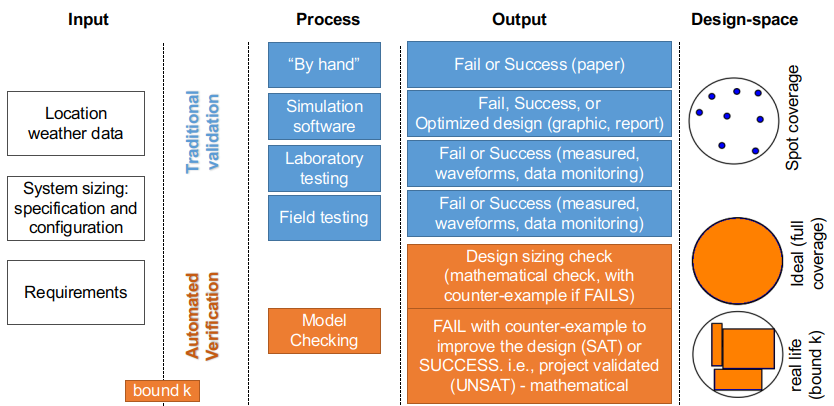
\includegraphics[width=1.0\textwidth]{PVprojectvalidation2}
\centering
\caption{Comparative of project validation methods}
\label{fig:validation}
\end{figure}

Starting at his point, it will be showed how is done the proposed automated verification of stand-alone solar PV systems. 

The process begins with the conversion of the real PV system into a model. The Fig. \ref{fig:systemverif4} shows how a real solar PV system is equivalent and converted to a model in order to be verified by a model checking. 

This illustration is a adaption from the general process of real system conversion depicted in Fig.~\ref{fig:systemverif}, detailing the inputs, outputs, and requirements of a real solar PV system. 

Worth to mention that the model checking process is the same independently of the system that is validated, and the important is to chose a accurate model, to define the requirements/constraints, and to get correct information from the system components, in order to get sound and effective validation,

\begin{figure}[h]
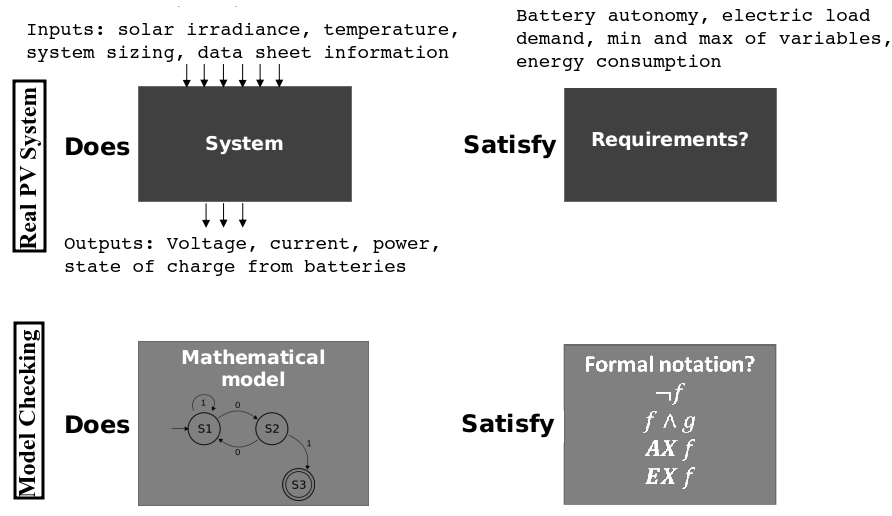
\includegraphics[width=0.8\textwidth]{systemverif4}
\centering
\caption{From real solar PV system verification to model checking. Source: adapted from \cite{Clarke2008}.}
\label{fig:systemverif4}
\end{figure}

Moreover, the proposed flowchart of the automated verification method is illustrated in Fig.~\ref{fig:flowchartgeneral}. Those three steps are the high level description of how the automated verification, applied to solar PV systems, works.

\begin{figure}[h]
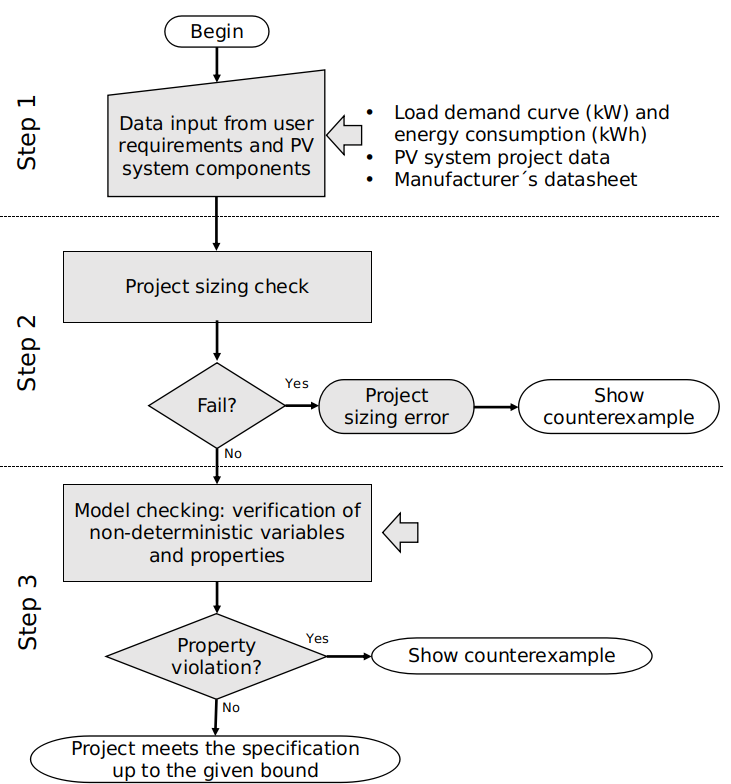
\includegraphics[width=0.6\textwidth]{flowchart_verification5.png}
\centering
\caption{Flowchart of the proposed automated verification of PV systems.}
\label{fig:flowchartgeneral}
\end{figure}

In \textbf{Step 1}, the PV input data %(e.g., load power demand and load energy consumption) 
and the formulae to check the sizing project, the mathematical model, the limits of the weather non-deterministic variables, are all written as an ANSI-C code~\cite{ANSI2018}. 

\textbf{Assumption:} All the PV system model, user requirements, assumptions, and technical information from the PV system equipment is written as an ANSI-C code.

In \textbf{Step 2}, the sizing check of the PV system takes place: it will indicate if there is an error of sizing before to perform the automated verification of the system. This stage ensures that the system meets the standard project steps related to critical period method of sizing~\cite{Pinho}. 

\textbf{Assumption:} before the automated verification, who performs the verification of the intended system behavior, is performed the sizing checking of the system. Moreover, if there is some error, the process stops, showing where is the sizing error.

\textbf{Assumption:} Sizing check is performed using critical period criteria.

In \textbf{Step 3}, weather variables (e.g., solar irradiance and ambient temperature) will be systematically explored by our verification engine based on maximum and minimum values from the site, where the PV system will be deployed. 
%As a consequence, all the formulae of the employed mathematical models will also be updated. 
In addition, depending on one of the desired properties of the system such as battery autonomy, energy availability, or even system power supply, our verification engine is able to indicate a failure if those properties are not met; in this particular case, it provides a diagnostic counterexample that shows in which conditions the property violation occurred. 
%; as the  state of charge of the batteries, load demand of power and the load consumption of energy if defined by the code
% (as reliability, performance, or safety)

%
%\textcolor{red}{In the following paragraph you should related the output of our verification engine with the description of the BMC SAT or UNSAR given above. For example, what does a failure mean? is it SAT?}
In a nutshell, the model checker will process the ANSI-C code with constraints ($C$) and properties ($P$) from the PV system, and the tool will automatically verify if the PV system requirements are met. If it returns a failure (i.e., SAT), then the tool provides a counterexample, i.e., a sequence of states that leads to the property violation; this information can be used as a feedback to improve the PV system design. However, if the verification succeeds (i.e., UNSAT), there is no failure up to the bound $k$; therefore, the PV system will present its intended behavior up to the bound $k$.

\textbf{Assumption:} Use of bound $k$ to restrict the design-space and improve performance.

%, i.e., our verification engine does not give any guarantee that there is no error in bound $k+1$ unless some induction method is employed~\cite{DBLP:journals/sttt/GadelhaIC17}.
%
%
%---------------------------------------------------------------------
% \subsection{The case studies and the Algorithm}
%---------------------------------------------------------------------
%
% 
%and as backup at night 
%
%The 700 W system: 3 x 325 W PV panels connected in series, controller of 150 V/35 A with a DC-bus of 24 V, 4 x 220 Ah batteries (2 in series and 2 in parallel arrangement), and inverter of 700 W. 
%
%And the 1,200 W PV system: 4 x 325 W connected in series PV panels, with controller of 150 V/35 A  in a DC-bus of 48 V, 4 batteries of 120 Ah connected in series, and a 1,200 W inverter.
%
%As demonstrated at this work, the performance of the system is highly dependent of solar irradiance and temperature, that are specific of the deployed local (latitude and longitude). 

Algorithm~\ref{alg:verification-algorithm} describes the equivalent pseudo-code. %Line 1 indicates a function call that performs the size checking of the each component of the PV system. %: using Equations \eqref{eq:NTPmin}, \eqref{eq:NTP}, \eqref{eq:NPSmin}, \eqref{eq:NPS}, \eqref{eq:NPP}, and \eqref{eq:NPPmin} to verify the PV panel; using \eqref{eq:Cbank}, \eqref{eq:Nbtotal}, and \eqref{eq:batcheck} to verify the batteries; using \eqref{eq:vcvsystem}, \eqref{eq:icmin}, and \eqref{eq:icicmin} to verify the charge controller; and using \eqref{eq:vindc}, \eqref{eq:voutac}, and \eqref{eq:invcheck} to verify the inverter. 
%The verification is carried out by the \textit{assert} macro from the ANSI-C programming language to encode each equation of sizing check. The argument to the \textit{assert} statement must be \textit{true} if the system specification is met; otherwise, the program aborts and prints a counterexample indicating a property violation. If there is no property violation, then the verification algorithm continues and 
In order to reduce the computational effort of the algorithm,
% caused by the state explosion inherent of the technique, 
every 24 h-day was considered as a time-step of 1 hour, and it was split into two parts: (a) one where it is possible to occur PV generation, during daylight, with a duration in hours depending on each site (but dependent on the sun and weather conditions); and (b) one that includes all the remaining day (without any PV generation), when the batteries are demanded to feed the house.

\textbf{Assumption:} day is divided in two parts (when there is and there is not PV generation, based in historical data from the location). Considering average temperature and solar irradiance (for every hour of the day) and the annual solar insolation (per day).

Lines 1 is devoted to information from the location where the PV system will be/were deployed. We use annual average minimum and maximum, related to temperature ($T$) and solar irradiance ($G$), hour by hour, from~\cite{Temperature}, and ~\cite{Irradiance}.

\textbf{Premise:} The availability of temperature, solar irradiance, and solar insolation data from the location where the solar PV system will be used.

Line 2 represents all the information that comes from the PV sizing and from the equipment manufacturers data: specification and data from PV, batteries, inverter and charge controller. This item includes as information from the house's load curve.

\textbf{Premise:} Availability of data sheet from every element of the solar PV system to be validated.

\textbf{Premise:} It is necessary the detailed sized project of the PV system in order to perform the validation (list of equipment and configuration, as voltage, current and how they are connected).

\textbf{Assumption:} Load curve from every house must be estimated or measured. Moreover, the time step is of 1 hour, and it is not considered seasonality, i.e., the load curve is the same for the entire year.

The first automated verification is related to the sizing check (line 3), if an error is found then the algorithm stops. In order to perform the sizing check, the algorithm uses Equations \eqref{eq:NTPmin}, \eqref{eq:NPSmin}, and \eqref{eq:NPPmin} to verify the PV panel; using \eqref{eq:Nbtotal}, and \eqref{eq:batcheck} to verify the batteries; using \eqref{eq:vcvsystem}, \eqref{eq:icmin}, and \eqref{eq:icicmin} to verify the charge controller; and using \eqref{eq:vindc}, \eqref{eq:voutac}, and \eqref{eq:invcheck} to verify the inverter.

Then, if there is not a sizing design flaw, two functions, called at lines 4 and 5, are responsible for discover which hour starts the PV generation and when stops. Those functions get this information from the array inputted to the Algorithm with the solar irradiance values.

The batteries are assumed to be charged, i.e., with SOC of 100\% (line 6).

\textbf{Assumption:} Batteries are considered charged at the beginning of the project validation.

The first for-loop at line 7 controls how many cycles of 24 h will be performed by the Algorithm.  And the for-loop from lines 8 to 11 is responsible to discharge the battery (according the load curve) and verify the state of charge of the battery, hour-by-hour, starting at the first hour of the day after the sun goes down until the next day before the sun goes up (without PV generation). Following, at the next for-loop, from line 12 to 29, is performed the verification where there is solar irradiance and all the PV system works. The Algorithm generates information related to average temperature ($T$) and solar irradiance ($G$), hour-by-hour, using non-deterministic variables from model checker to explore all possible states and the \textit{assume} macro to constrain the non-deterministic values using a given range (lines 15 and 16). 
%and irradiance varies from 0 W/m$^{2}$ to 852 W/m$^{2}$ (with minimum of 274 W/m$^{2}$ during the daytime, when there is sunlight). 
%there is PV generation only between 8:00 h and 16:00 h every day, 
%with zero electric energy generation from 18:00 h to 6:00 h of the next day; and with insignificant generation from 6:00 h to 8:00 h, and from 16:00 h to 18:00 h of the same day. 

After that, the model from PV generator is used in the function call of line 17, to produce the voltage and current considering the states of $G$ and $T$. With respect to every hour considered, the conditional \textit{if-elseif-endif} statements from lines 18, 20, 22, 24 and 26, will imitate the charge controller work as depicted in Table~\ref{table:controller} of Section~\ref{sec:controller}, performing the charge or discharge of batteries according to the value of different variables: if there is PV generation, the updated state of charge from batteries, the house's load and the set-up information of the PV system.

At the end of last for-loop, the state of the batteries is verified again (line 27) and the hour is adjusted to the next loop (line 28).

Nevertheless, if the verification engine does not fail, we can conclude that the PV system does not need further corrections up to the given bound $k$.
%
%\textcolor{red}{this sentence is unclear... After this process is started the battery autonomy verification, from line 31}. \textcolor{red}{this sentence is unclear... Based on the fact that won't be PV generation after a given time of the day, the algorithm will only discharge the batteries until a new charging process (at the next day) to start.} \textcolor{red}{what do you mean by The formal verification is guaranteed?...  The formal verification is guaranteed by  macro to specific variables of the model, according lines 27 and 35.}
% and the non-deterministic variables $G$ and $T$ are considered during the formal verification of the system, otherwise, during the other two periods, there is no PV generation and just the power consumption from the backup batteries. 
%Within this 8h-period, $G$ and $T$ are automated verified with different values every one hour.
%, and change their value every 1 h according with the algorithm created using the technique.
 \begin{algorithm}
 \caption{Model checking algorithm for validation of stand-alone PV systems}
 \begin{algorithmic}[1]
 \begin{scriptsize}
 \renewcommand{\algorithmicrequire}{\textbf{Input:}}
 \renewcommand{\algorithmicensure}{\textbf{Output:}}
  \STATE $declare \, min \, and \, max \, solar \, irradiation[24h], \, and \, temperature[24h]$\\
  \STATE $declare \, case \, studies \, details: \, sizing \, and \, manufacturers \, data $ \\
  \STATE $sizing \_ check()$ \\
  \STATE $startPVgeneration \leftarrow findStartPVgeneration()$ \\
  \STATE $endPVgeneration \leftarrow findEndPVgeneration()$ \\
  \STATE $SOC \leftarrow 100\%$ \\
%  \COMMENT {Starting with the PV generation time}
% \\ 
%\textit{LOOP Process}
 \FOR {$1st \, 24h \, loop$ to $Nth \, 24h \, loop$}
  \FOR {$endPVgeneration+1$ to $startPVgeneration-1$}
	  \STATE $dischargeBattery \, in \, 1h()$ \\
%	  \STATE $autonomyCount \leftarrow autonomyCount+1$ \\
	  \STATE $assert (SOC \geq SOC \_ min)$ \\
%	  \STATE $battery \, autonomy \, verification()$ \\
  \ENDFOR
  \FOR {$startPVgeneration$ to $endPVgeneration$}
    \STATE $G \leftarrow nondet \_ uint(\,)$ \COMMENT {$G$ is non-deterministic variable}
    \STATE $T \leftarrow nondet \_ uint(\,)$ \COMMENT {$T$ is non-deterministic variable}
    \STATE assume ($Gmin \leq G \leq Gmax$) \COMMENT {restricting $G$ values}
    \STATE assume ($Tmin \leq T \leq Tmax$) \COMMENT {restricting $T$ values}
    \STATE $Imax, Vmax \leftarrow PVgenerationMODEL (G,T)$ \\
    \COMMENT {If-then-else sequence to imitate charge controller work}
    \IF {($battery \, is \, empty$) AND ($PV \, is \, generating$)}
      \STATE $chargeBattery \, in \, 1h()$ \COMMENT {PV feed the house}
    \ELSIF {($battery \, is \, empty$) AND NOT($PV \, is \, generating$)}
      \STATE FAIL with assert macro \COMMENT {Battery is empty and there is not PV generation}
    \ELSIF {NOT($battery \, is \, empty$) AND ($PV \, is \, generating$)}
      \STATE stop battery charge \COMMENT {PV feed the house}
    \ELSIF {NOT($battery \, is \, empty$) AND NOT($PV \, is \, generating$)}
      \STATE $dischargeBattery \, in \, 1h()$ \COMMENT {Battery feed the house}
    \ENDIF
    \STATE $assert (SOC \geq SOC \_ min)$ \\
    \STATE $hour \leftarrow hour+1$ \\
   \ENDFOR
  \ENDFOR
 \RETURN $(\,)$ 
  \end{scriptsize}
 \end{algorithmic} 
 \label{alg:verification-algorithm}
 \end{algorithm}

%\subsubsection{Assumptions and Premises} 
%

\section{Optimal Sizing of Solar PV Systems}

Fig.~\ref{fig:optimization} illustrates how to obtain the optimal sizing of a stand-alone solar PV system, passing through the traditional techniques (manual, and simulation), and including the proposed automatic synthesis that is detailed in this Section. 

One more time, as depicted in automated verification process, the input information is the same for all the methods, with the difference that in automated validation it is possible to define the bound $k$ to restrict the design-space search. And the outputs are not equal, as the design-space coverage and the, mainly, the final resulting.

\begin{figure}[h]
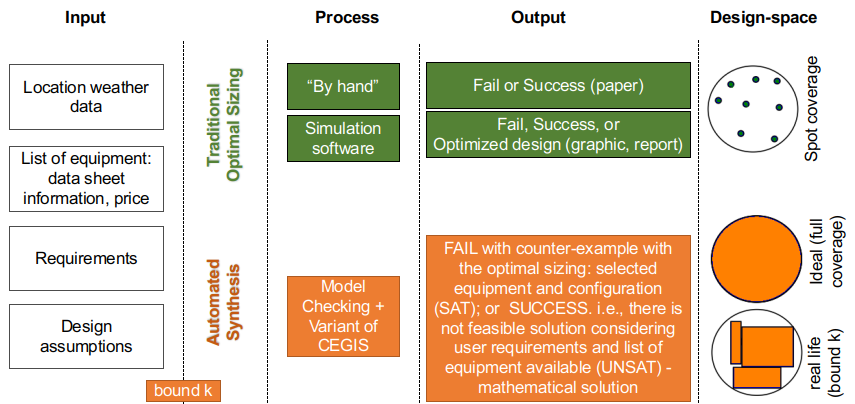
\includegraphics[width=1.0\textwidth]{optimalsizingprocess2}
\centering
\caption{Comparative of optimal sizing methods}
\label{fig:optimization}
\end{figure}
 
\subsection{Variant of CEGIS} 

In Figure~\ref{CEGISalt}, it is pictured a variant of CEGIS previously presented in Section ~\ref{sec:ProgramSynthesis}, Fig.~\ref{Counter-Example-Guided-Inductive-Synthesis}. This variant was created during this Thesis and it will be detailed in this Section.

\begin{figure}[h]
	\centering
	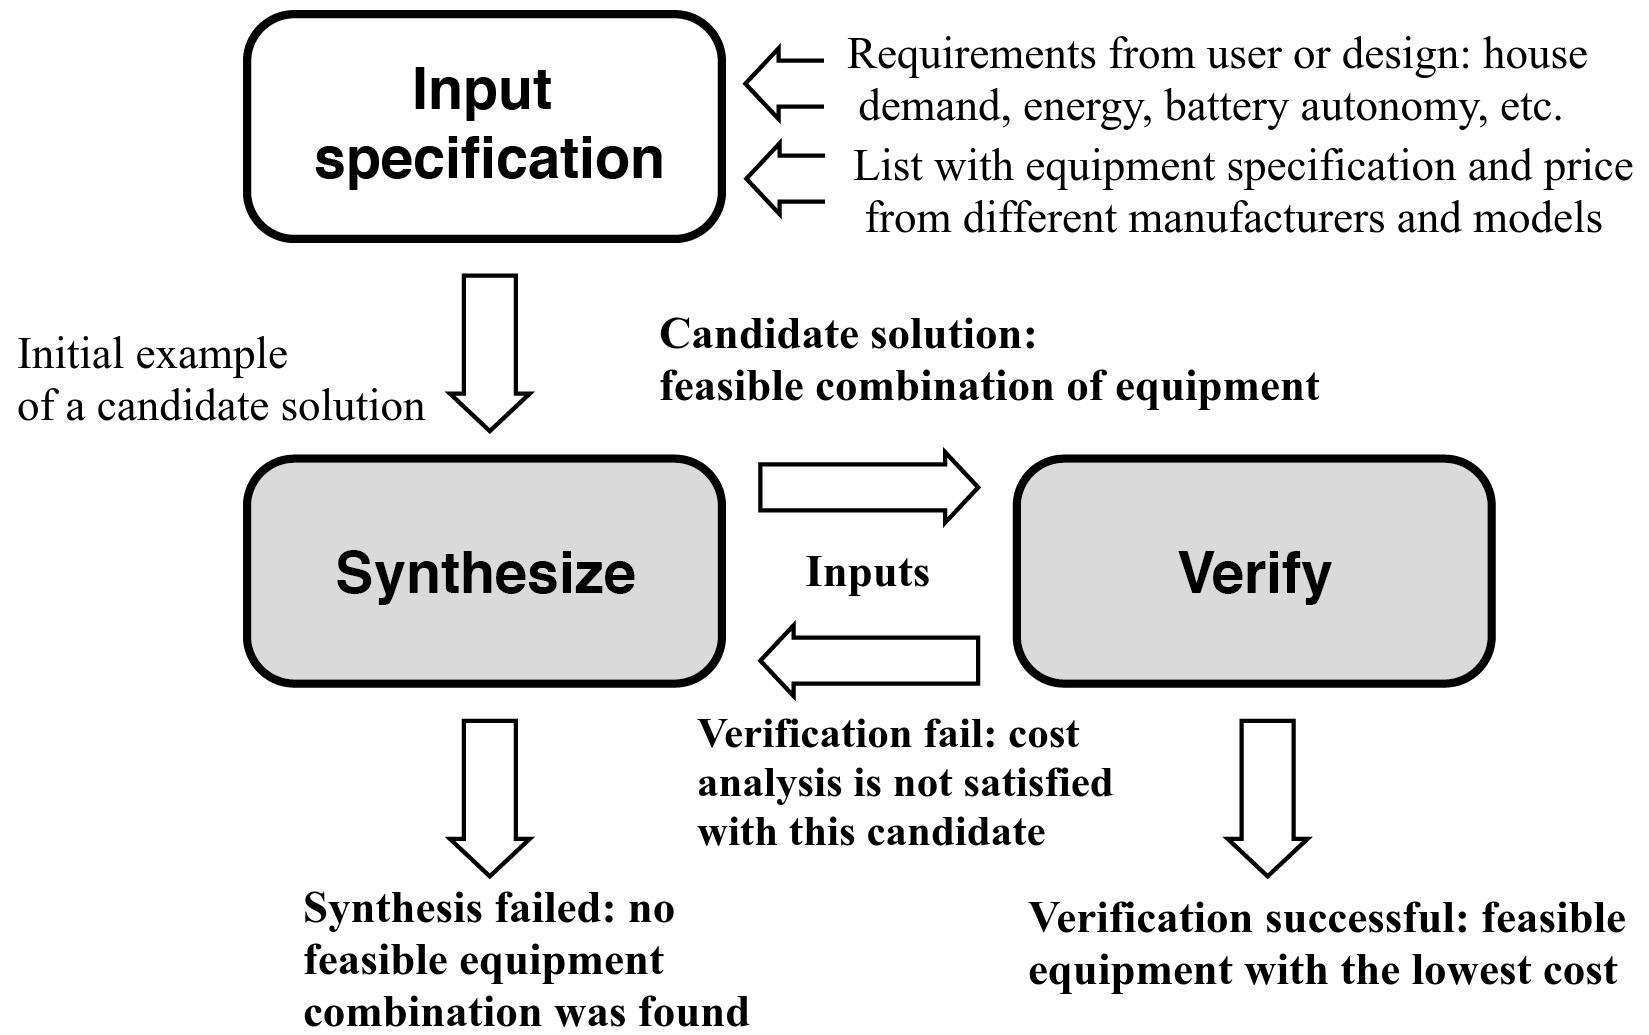
\includegraphics[width=0.75\columnwidth]{fig2_rev.jpg}
	\caption{CEGIS applied to PV system sizing.}
	\label{CEGISalt}
\end{figure}

Examples of specification used by the proposed method include solar insolation (site dependent), house power demand, house consumption energy, estimated load curve, AC voltage, and battery autonomy; we also provide a list of equipment specification and price from different manufacturers and models. Design assumptions are considered project specification as well. The assumptions regarding the optimal sizing are listed in Section~\ref{sec:OptAssumptions}.

There are four particular differences related to the traditional CEGIS described in Figure ~\ref{Counter-Example-Guided-Inductive-Synthesis} when compared to the variant CEGIS used in the proposed approach: 

\begin{itemize}
\item There exists no test vector and every candidate is generated during the run-time in the {\sc Synthesize} phase and sent to the {\sc Verify} phase; 
\item If the {\sc Verify} phase is unsuccessful, then a new candidate is generated by {\sc Synthesize} 
\item The lower bound of the {\sc Verify} phase is incremented to search for the lowest cost; 
\item As a result, there exists no refinement from the {\sc Verify} phase back to the {\sc Synthesize} phase, i.e., a new counterexample is not added to the {\sc input} set since a failure during the {\sc Verify} phase will only discard a given candidate that could be feasible in the next iteration with a new lower bound.
\end{itemize}

Program synthesis engines that implement the CEGIS approach~\cite{sketch} can automatically produce solutions for a large variety of specifications; here we have used symbolic software verifiers based on SMT solvers.


Algorithm~\ref{alg:opt-algorithm} describes our pseudo-code to synthesize stand-alone PV systems using symbolic model checking. It was adopted the analytical method of optimization, with LCC economical analysis and power reliability based on the critical period criteria.
%
 \begin{algorithm}
 \caption{Synthesis algorithm}
 \begin{algorithmic}[1]
 \renewcommand{\algorithmicrequire}{\textbf{Input:}}
 \renewcommand{\algorithmicensure}{\textbf{Output:}}
  \STATE Initialize variables \\
  \STATE Declare list of PV panels, controllers, batteries, and inverters data and cost \\
%  \STATE Declare list of controllers data and cost \\
%  \STATE Declare list of batteries data and cost \\
%  \STATE Declare list of inverters data and cost \\
  \STATE Declare the maximum possible cost $MaxCost$  \\
  \STATE Declare power demand, power peak, energy consumption \\
  \STATE Declare battery autonomy, deep of discharge, AC voltage \\
  \FOR {$HintCost=0$ to $MaxCost$}
 	\STATE Declare non-deterministic variable to select PV Panel from list \\
 	\STATE Declare non-deterministic variable to select Controller from list \\
 	\STATE Declare non-deterministic variable to select Battery from list \\
 	\STATE Declare non-deterministic variable to select Inverter from list \\ 	
 	\STATE Calculate $E_{corrected}, \, E_{p} $ \\
	\STATE Calculate $N_{TPmin}, \, N_{PSmin}, N_{PPmin} $ \\
 	\STATE Calculate $C_{bank}$ \\
	\STATE Calculate $N_{BS}min, \, N_{BP}min, \, N_{B}total$ \\
	\STATE Requirement enforced by \textbf{assume}$(V_{c})$ \\
 	\STATE Calculate $I_{sc,amb}$ \\
 	\STATE Calculate $I_{c,min}$ \\
 	\STATE Requirement enforced by \textbf{assume}$(I_{c} \wedge V_{in}DC \wedge V_{out}AC)$ \\
%	\STATE Requirement enforced by \textbf{assume}$(V_{in}DC \wedge V_{out}AC )$ \\
%	\STATE Requirement enforced by \textbf{assume}$(V_{out}AC)$ \\
	\STATE Requirement enforced by \textbf{assume}$(Demand \wedge P_{surge})$ \\
%	\STATE Requirement enforced by \textbf{assume}$(P_{surge})$ \\
	\STATE non-deterministic variables hold feasible equipment and cost  \\
	\STATE $F_{obj} \leftarrow  N_{TP}*Panel_{Cost} \, + \, N_{TB}*Battery_{Cost} \, + Controller_{Cost} \, + \, Inverter_{Cost} \, + \, Installation_{Cost} \, + \, batrep_{Cost} \, + \, PWO\&M_{Cost}$ \\
	\STATE Violation check with \textbf{assert}$(F_{obj} > HintCost)$ \\
  \ENDFOR
 \RETURN $(\,)$ 
 \end{algorithmic} 
 \label{alg:opt-algorithm}
 \end{algorithm}
%

Our synthesis algorithm will synthesize constant values; 
it starts with the input of manufacturers data and prices of PV panels, batteries, 
charge controllers and inverters (line $2$). After that, we define user requirements, i.e., 
house requirements and design definitions, from lines $4$ and $5$. 

The \textit{for}-loop started at line $6$ controls the lowest cost to the PV solution. 
In particular, it starts with cost $0$ and stops only when the algorithm finds a 
feasible solution in which the cost breaks the $assertion$ stated in line $22$; 
if that happens, then our algorithm has found an optimal solution, thereby stating 
that the {\sc Verify} phase reached a satisfiable condition (\textit{SAT}). 
The $MaxCost$ value at line $6$ is just a very high value put as a limit 
to the \textit{for}-loop, that never will be reached because the optimal solution will be found first.

Our synthesis algorithm uses non-deterministic variables to choose one specific constant 
from a given list of PV panels, controllers, batteries and inverters (lines $7$ to $10$). 
That procedure ensures that our synthesis engine checks all combinations of items 
from each equipment, and combine them to assemble a feasible (candidate) PV solution, 
which meets the user requirements.

Next, we use Eq.~\eqref{eq:Ecorrected}, Eq.~\eqref{eq:Ep}, Eq.~\eqref{eq:NTPmin}, 
Eq.~\eqref{eq:NPSmin}, Eq.~\eqref{eq:NPPmin}, Eq.~\eqref{eq:Cbank}, 
Eq.~\eqref{eq:Nbtotal}, Eq.~\eqref{eq:iscamb}, and Eq.~\eqref{eq:icmin} to calculate the sizing variables (lines $11$ to $17$). The directive \textit{assume} (lines $15$, $18$ and $19$) 
ensures the compatibility of the chosen items from the list of equipment: the {\sc Verify} phase 
uses only the item (among all the possible ones) that satisfies the statements of Lines $15$, $18$ and $19$. Line $15$ is specific to the charge controller voltage check. Line $18$ checks the inverter check $I_{c}$, charge controller DC input voltage $V_{in}DC$, and charge controller AC output voltage $V_{in}DC$ check. Line $19$ ensures the power demand and the surge power of inverter.
Therefore, our synthesis algorithm reaches line $20$ with one feasible solution, 
and the cost of that solution is calculated in $F_{obj}$ (line $21$). This cost is the equivalent of ~\ref{eq:LCC} described in Section ~\ref{sec:optcriteria}.

If our algorithm does not find a feasible solution among the item of equipment that 
were provided to our {\sc Synthesize} phase,  then the result is an unsatisfiable (\textit{UNSAT}), i.e., 
the program finishes and does not find a solution, which indicates that it 
was not possible to combine the items of each equipment in order to create a feasible solution. 

The main challenge for the {\sc Synthesize} phase is to find a feasible candidate 
solution regarding the constraints and user requirements. Related to our {\sc Verify} 
phase the challenge is to find the lowest acquisition cost from a list of equipment and 
components that is provided from the {\sc Synthesize} phase. 

Note that the process described here is completely automated and that a validation is performed 
by our {\sc Verify} phase to ensure that the approach is sound.

\subsection{Optimization Assumptions and Premises}
\label{sec:OptAssumptions}
%%%%%%%%%%%%%%%%%%%%%%%%%%%%%%%

Here some premise are presented and some adopted assumptions are explained for the optimal sizing method, regarding the automated synthesis and simulation software.

Regarding the line $2$ of Algorithm~\ref{alg:verification-algorithm}, 
a list of forty equipment from ten different manufacturers was provided 
to the synthesis engine in order to allow the choice of every item 
of PV sizing. Data sheet from each item was necessary to collect 
technical information. Moreover, the price of each item was obtained 
from available quotations in the market, and if the currency was not in US dollars, 
then it was used the exchange rate of the day to convert it to US dollars.

With respect to power reliability, this work will rely on the critical period solar 
energy method~\cite{Pinho} as described in Section~\ref{sec:sizing}. 
The usual way is to use loss of load probability (LOLP) or loss of power 
supply probability (LPSP). However, based on the fact that here we 
are neither considering site characteristics nor the load changes over time, 
which demands historical data, the reliability analysis will be developed only 
by the critical period method of PV sizing.

Regarding financial analysis:
\begin{itemize}
	\item LCC lifetime considered: $20$ years;
	\item Installation costs: includes delivery in the isolated community and installation costs itself, $5$\% of total cost~\cite{Agrener2013};
	\item Value of the discount rate or interest rate: $10$\%, which is a good rate considering financial investments in developing countries;
	\item Operation and maintenance annual costs: based on past PV projects of similar size in the Amazon region of Brazil, will be adopted the value of US\$ 289.64~\cite{Agrener2013}. This cost includes the battery replacement based on its lifetime ($4$ years for lead-acid batteries), plus inverters and controller replacement (every $10$ years). Therefore, it will be performed three battery bank and one inverter-controller replacements during the LCC analysis.
\end{itemize}

On the subject of PV system optimization technique, we will adopt here the intuitive method 
since the average value daily of solar irradiance is used in the mathematical model, 
without considering the battery's state of charge, or even the random nature 
of solar irradiation and meteorological conditions. Therefore, all the computational 
effort will be concentrated in our automated synthesis algorithm.

Regarding all case studies, it was defined that the minimum state of charge of batteries is $75$\% (with DOD maximum of $25$\%, which is common to lead-acid batteries), the voltage of the system is set in $24$ V DC (the most common as well, but the value can be adjusted to $12$ or $48$ V at the code), and the AC voltage from the inverter is $127$ V (Brazilian standard).

Related to off-the-shelf simulation tools only HOMER Pro and Hybrid2 perform off-grid system with battery backup analysis. Additionally, HOMER and RETScreen include economical analysis or even optimization-sensitive analysis. Therefore, in this study, HOMER Pro will be the simulation tool used to compare with our automated synthesis method.  Related to HOMER Pro:

\begin{itemize}
	\item HOMER Pro do not have the LCC cost in its reports. However, it has NPC and LCOE. Therefore NPC was used to obtain LCC in order to allow the comparative among tools;
	\item The optimization analysis of HOMER Pro allows to define a load curve and temperature according of data collected automatically from online databases. However, in order to allow a correct comparative, the curve load and the temperature were defined exactly the same as automated synthesis tools;
	\item Battery autonomy is not an parameter that the user can set when using HOMER Pro. The tool will always to meet the user requirement, i.e., the load curve during the $365$ days of the year;
	\item HOMER Pro do not have a explicit equipment called charge controller. It uses a controller resource that can perform in two different ways, according of the optimization choice or the user choice: load following or cycle charging~\cite{HOMER}. During the tests it was chosen the load following controller: it produces only enough power to meet the demand~\cite{HOMER};
	\item It was assumed the value of 5\% of capacity shortage that is equivalent to 95\% of availability of the PV system. By definition, availability is the percentage of time at which a power system is capable of meeting the load requirements~\cite{Khatib2014}. For critical loads, 99\% is considered acceptable. While in a ordinary house electrical load, 95\% is considered acceptable;
	\item It was assumed a string of two batteries in order to match the voltage of the system of $24$ V DC that was used for the automated synthesis tool;
	\item The premise adopted when using HOMER Pro it was that the user does not know the optimal solution, and that in order to obtain this solution is necessary to include (at the design phase of the tool) generic PV and batteries modules that HOMER Pro will search for the optimized power of each component. With that in mind, it was included a generic flat plate PV of $1$ kW and generic lead-acid batteries of $1$ kW as well (and with capacity of $83.4$ Ah according with HOMER Pro modeling). HOMER, during run-time, decides the size in kW of each module, based on feasibility and lower cost.
\end{itemize}

\section{Conclusion}

This Chapter showed in details how the automated verification method and the automated synthesis method, two state-of-art tools used in computer science, were adapted in order to be used in stand-alone solar PV systems to validate their behavior or the obtain the optimal project sizing. Moreover, is was possible to picture how the proposed methods are compared with the traditional ones used for the same purpose.

Detailed diagrams, flowcharts and algorithms with pseudo-code were presented with the aim to support the proposed work and to facilitate the understanding. And even more so, the assumptions adopted for the automated verification and simulation software were listed, because those assumptions have impact at the results there will be presented at the next two Chapters.


%
%\chapter{Automated Synthesis Methodology}
%\label{chap:methodology2}
%This Chapter is devoted to the results of using automated verification to validate the intended behavior of stand-alone solar PV systems. Moreover, there is the comparative with a specialized simulation tool, and even the use of different verifiers who perform the automated verification in order to evaluate performance. Tables, commented reports, and graphical outputs are presented to aid the understanding.

\section{Description of the Case Studies}
%------------------------------------------
%
%We have performed five case studies to evaluate our proposed verification method: (a) four PV systems (three in series 325W PV panels, four 220 Ah batteries in a configuration with two series and two parallel with 48h autonomy, 700 W inverter with peak power of 1,600W, charge controller with MPPT with 35A/150V of capacity) deployed in four different houses in an indigenous community (GPS coordinates 2$^{o}$44'50.0"S 60$^{o}$25'47.8"W) situated nearby Manaus (Brazil), with each house having a different power demand (house 1 = 253 W, house 2 = 263 W, house 3 = 283 W, and house 4 = 501 W); and (b) one case concerning a system deployed as an individual system in Manaus (GPS coordinates 3$^{o}$4'20.208"S 60$^{o}$0'30.168"W), supporting 915 W of the house's load (house 5 with four 325W PV panels in a configuration two series and two parallel, four 120Ah batteries in series and autonomy of just 6 h, 1,200 W inverter with surge of 1,600 W, charge controller with MPPT of 150V/35A). 
We have performed five case studies to evaluate the proposed approach as described in Table~\ref{tab2}. %Furthermore, three start-of-art verification tools, as described in Section~\ref{sec:AutomatedVerification} (ESBMC, CBMC, and CPAchecker), and HOMER Pro simulation tool were used to compare the approach effectiveness and efficiency.
These case studies were defined based on usual electrical load found in riverside communities of the Amazon State in Brazil~\cite{abs-1811-09438, Agrener2013}.

Worth to mention that the load curve represents a array of 24 integer numbers for every hour of the day (instant power in Watts) and it was estimated after visiting and survey applied in June of 2017, before the houses were electrified.

\begin{table}
\caption{Case studies: stand-alone solar PV systems.}\label{tab2}
\begin{scriptsize}
\begin{tabular}{|c|c|c|c|c|c|}
\hline
\hline
Item & House 1 & House 2 & House 3 & House 4 & House 5\\
\hline
\hline
PV Panels &  \multicolumn{4}{|c|}{3$\times$325 W: (3S)} & 4$\times$325 W: (2S-2P) \\
\hline
Batteries & \multicolumn{4}{|c|}{\makecell{4$\times$220 Ah: (2S-2P)\\ autonomy: 48 h}} & \makecell{4$\times$120 Ah: (4S)\\ autonomy: 6 h}\\
\hline
Charge Controller & \multicolumn{5}{|c|}{With MPPT of 150 V/35 A}\\
\hline
Inverter & \multicolumn{4}{|c|}{700 W, surge: 1,600 W} & 1,200 W, surge: 1,600 W\\
\hline
Power peak (W)& 342  & 253  & 263 & 322 & 814 \\
\hline
Power surge (W)& 342 & 722 & 732 & 896 & 980\\
\hline
Load curve (W) & \multicolumn{5}{|l|}{\makecell{House 1: 118-118-118-46-46-46-95-95-170-170-296-242-242-95-95-95-95-95-342-288-288-288-288-118\\House 2: 136-136-136-136-136-136-67-67-184-184-184-184-184-67-67-67-67-67-253-253-253-253-253-136\\House 3: 113-113-113-113-113-113-67-67-217-97-97-97-97-97-97-97-97-97-263-113-113-113-113-113\\House 4: 207-207-207-135-135-135-66-66-161-161-233-253-248-66-66-66-66-66-302-317-322-302-302-207\\House 5: 45-16-16-16-16-16-0-0-0-72-72-222-150-150-0-0-72-72-814-814-814-742-742-16}}\\
\hline
\makecell{Consumption\\ (kWh/day)}& 3.9 & 3.6 & 2.5 & 4.3 & 4.88\\
\hline
GPS Coordinates & \multicolumn{4}{|c|}{\makecell{2$^{o}$44'50.0"S 60$^{o}$25'47.8"W\\}} & \makecell{3$^{o}$4'20.208"S \\60$^{o}$0'30.168"W}\\
\hline
Details & \multicolumn{4}{|c|}{\makecell{Riverside indigenous community\\Rural Area of Manaus - Brazil}} & \makecell{Urban house \\Manaus-Amazonas-Brazil}\\
\hline
\hline
\end{tabular}
Legend: (S): Series; (P): Parallel.
\end{scriptsize}
\end{table}

%------------------------------------------
\section{Objectives and Setup}
\label{sec:setup}
%------------------------------------------

The experimental evaluation aims to answer two research questions:
%
\begin{enumerate}
\item[RQ1] \textbf{(soundness)} Does the automated verification approach provide correct results?
\item[RQ2] \textbf{(performance)} How do the verifiers compare to each other and to a simulation commercial tool?
\end{enumerate}

%In order to evaluate the proposed verification method and its performance, we have considered five case studies, three verification engines in different configurations, and also compared the results to the HOMER Pro tool. All the experiments were performed with a time out of 14,400 seconds. %Every dweller, who owns a PV system, was interviewed 
%
All experiments were conducted on an otherwise idle Intel Xeon CPU E5-4617 (8-cores) with 2.90 GHz and 64 GB of RAM, running Ubuntu 16.04 LTS 64-bits. The setup of HOMER Pro v3.13.1 was an Intel Core i5-4210 (4-cores), with 1.7 GHz and 4 GB of RAM, running Windows 10. The experiments were performed with time out of 240 minutes.

Verification engine ESBMC, version v6.0.0 was used with the SMT solver Boolector version 3.0.1~\cite{Brummayer}\footnote{Command-line: \$ esbmc filename.c -\phantom{}-no-bounds-check -\phantom{}-no-pointer-check -\phantom{}-unwind 100 -\phantom{}-boolector}; and an alternative ESBMC v6.0.0 was used with the SMT incremental mode\footnote{Command-line: \$ esbmc filename.c -\phantom{}-no-bounds-check -\phantom{}-no-pointer-check -\phantom{}-unwind 100 -\phantom{}-smt-during-symex -\phantom{}-smt-symex-guard -\phantom{}-z3} enabled; with SMT solver Z3 version 4.7.1~\cite{DeMoura}. % with the goal of reducing memory usage.

Verification engine CBMC 5.11 and MiniSat 2.2.1 were used in the comparison~\cite{Kroening}\footnote{Command-line: \$ cbmc filename.c -\phantom{}-unwind 100 -\phantom{}-trace}.
 
Verification engine CPAchecker 1.8 was used \footnote{Command-line: \$ scripts/cpa.sh -heap 64000m -stack 10240k -config config/bmc-incremental.properties -spec config/specification/sv-comp-reachability.spc filename.c}, with the SMT solver MathSAT version 5.5.3~\cite{mathsat5}. An alternative CPAchecker configuration was tried as well, using BMC k-induction option, but without improvements of performance or soundness in the results (so it is not reported here).

%\section{Verifiers Environment}
%\label{sec:verifenviron}

%------------------------------------------
\section{Results and Discussion}
\label{sec:results_indeed}
%------------------------------------------

This Section presents the results, with commented outputs produced by every tool, mainly related to the reports (CBMC and ESBMC) and some graphical resources (CPAchecker and ESBMC).

%\textcolor{red}{We should answer the two% research questions here... please take a look at https://ssvlab.github.io/lucasccordeiro/papers/cav2017.pdf to check how you can answer.}
%\begin{enumerate}
%\item[RQ1] \textbf{(soundness)} Does our approach provide correct results?
%\item[RQ2] \textbf{(performance)} How does our approach compare against other existing tools?
%
Table~\ref{cases} summarizes the results. The times reported in Table~\ref{cases} answer RQ2. 
Note that an UNKNOWN result from the proposed verification engines does not mean that a failure was found neither that the verification is successful: it indicates that the verification engine led to an \textit{out of memory} or a \textit{time out} situation.

%HOMER Pro result: the $1,200$W was the only one that was proved to not meet the requirement of battery autonomy; all the 700W systems had no indication of flaws during simulation. The simulation took less than five seconds to be performed on each case study.
%
\begin{table}
\centering
\caption{Summary of the case-studies comparative and the automated tools.}\label{cases}
\begin{scriptsize}
\begin{tabular}{|c|c|c|c|c|}
\hline
\hline
\multicolumn{5}{|c|}{Model Checker (SAT/UNSAT: time and message)}\\
\hline
Case &  \makecell{ESBMC 6.0.0\\(Boolector 3.0.1)} & \makecell {ESBMC 6.0.0\\(Z3 4.7.1)} & \makecell{CBMC 5.11\\(MiniSat 2.2.1)} & \makecell{CPAchecker 1.8\\(MathSAT 5.5.3)}\\
\hline
\hline
House 1 &  \makecell{Out of memory \\(UNKNOWN)} & \makecell{05 m 08 s \\(UNSAT)} & \makecell{19 m 02 s \\(UNSAT)} & \makecell{Time out \\ (UNKNOWN)}\\
\hline
House 2 &  \makecell{Out of memory \\(UNKNOWN)} & \makecell{04 m 27 s \\(UNSAT)} & \makecell{18 m 59 s \\(UNSAT)} & \makecell{Time out \\ (UNKNOWN)}\\
\hline
House 3 &  \makecell{Out of memory \\(UNKNOWN)} & \makecell{05 m 07 s \\(UNSAT)} & \makecell{18 m 39 s \\(UNSAT)} & \makecell{Time out \\ (UNKNOWN)}\\
\hline
House 4 &  \makecell{Out of memory \\(UNKNOWN)} & \makecell{04 m 37 s \\(UNSAT)} & \makecell{18 m 36 s \\(UNSAT)} & \makecell{Time out \\ (UNKNOWN)}\\
\hline
House 5 &  \makecell{Out of memory \\(UNKNOWN)} & \makecell{$\leq$ 1 sec \\(SAT Line 337)} & \makecell{$\leq$ 1 sec \\(SAT Line 337)} & \makecell{6 sec \\ (SAT line 337)}\\
\hline
\hline
\end{tabular}
\end{scriptsize}
\end{table}

The description of the experimental results can be broken down into three parts, one for each verification engine: ESBMC, CBMC, and CPAchecker. 

\subsection{ESBMC}
Related to ESBMC, we have tried two possibilities: one with Boolector and another one with Z3. The incremental option, which uses less memory, can be performed with Z3 only since ESBMC does not support the incremental mode with Boolector yet. 

Using ESBMC with Boolector led to an out of memory situation in all the case studies. This result was obtained in less than six minutes of execution, i.e., the 64 GB of RAM were consumed by the verification engine and the processes were killed, thus leading to an UNKNOWN result returned by ESBMC as shown in the first column of Table~\ref{cases}. 

However, running the same version of ESBMC but using incremental solving with Z3, the experimentation returned was conclusive (SAT or UNSAT) to all the case studies. 

Related to the cases that use a 700 W PV system (house 1, house 2, house 3, and house 4), ESBMC could not reach an error in all the four houses and the execution time took from 04 m 27 s to 05 m 08 s. Fig.~\ref{fig:esbmcverifhouse1} shows the output report of the tool for the house 1, with the absence of fail at the end of analysis. The file produced by ESBMC is 160 lines long and 12.4 kB of size. The author highlighted the result, which shows that was not found design flaws (SAT result or SUCCESS) within the bound $k$ of 100.

\begin{figure}[h]
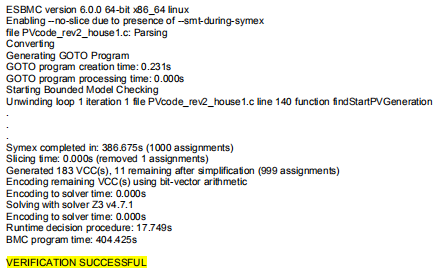
\includegraphics[width=0.65\textwidth]{esbmcverifh1.png}
\centering
\caption{Report generated by ESBMC (with Z3 solver) after validation of House 1.}
\label{fig:esbmcverifhouse1}
\end{figure}

However the 1,200 W PV system (house 5) failed (SAT) in line 337 of the code, thereby indicating that the system is \textit{incorrectly} sized; in particular, the counterexample provided by the verification engine indicated that the nominal current from the charge controller is less than the minimum current demanded by the PV system, therefore the equipment chosen is not suitable to meet the design requirements.

Fig.~\ref{fig:esbmcverifhouse5} shows the report issued by the tool, with red highlights for the result, showing the incompatibility of the sized charge controller and the minimum necessary. The report generated by ESBMC was a text file of 14.1 kB of size and 353 lines of length. This verification took less than 1 s to be performed, as indicated in the last line of Table~\ref{cases}, and it is faster than the previous analysis because ESBMC stops during the sizing check, which is in line 3 of Algorithm~\ref{alg:verification-algorithm}, and does not perform the rest of verification code.

\begin{figure}[h]
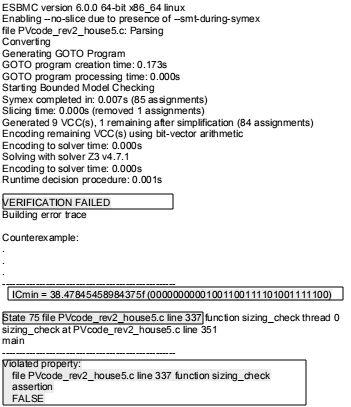
\includegraphics[width=0.65\textwidth]{esbmcverifh5.png}
\centering
\caption{Report generated by ESBMC (with Z3 solver) after validation of House 5.}
\label{fig:esbmcverifhouse5}
\end{figure}

%At the terminal, the command used to perform the verification is:
%\$ esbmc filename.c -\phantom{}-no-bounds-check -\phantom{}-no-pointer-check -\phantom{}-no-div-by-zero-check -\phantom{}-unwind 300 -\phantom{}-smt-during-symex -\phantom{}-smt-symex-guard --z3
%
%Where:
%
%\begin{itemize}
%\item The first three parameters, after the filename, are related to options that are usual to find bug in software, %for example, like bound check to arrays, pointer check, and division by zero, 
%but unnecessary to check at this kind of problem (if not removed, there is lost of performance during the automated verification);
%\item The parameter $unmind$ tells to ESBMC the limit to unroll the loops. This number was optimized (empirically) in order to reduce the running time and avoid to unwind unnecessarily the loops;
%\item The two parameters with $symex$ tell to ESBMC to perform an incremental SMT solving. There are other options, but this parameter is necessary because the complexity of the algorithms. The incremental SMT solving uses few RAM memory, compared with other SMT solving. 
%During empirical tests of the algorithms, the incremental solving was the only one who do not demanded 100\% the RAM memory. The use of swap-memory, i.e., the use of hard disk, reduces the performance and must be avoided;
%\item And the last parameter says to the tool that the Z3 SMT solver will be used.
%\end{itemize}
%


\subsection{CBMC}

Concerning the CBMC tool, similar results were obtained, but with some slower time than ESBMC. The experimentation returned SAT or UNSAT to all the case studies, i.e., it was conclusive to all houses. 

Related to the 700 W PV systems (house 1, house 2, house 3, and house 4), the tool could not reach an error in all the four houses and the execution time took from 18 m 36 s to 19 m 02 s. 

Fig. \ref{fig:cbmcverifhouse1} shows part of report produced by CBMC when validating the house 1. The file produced by CBMC is 270,512 lines long and 39 MB of size. The author highlighted the result, which shows that was not found design flaws within the bound $k$ of 100.

\begin{figure}[h]
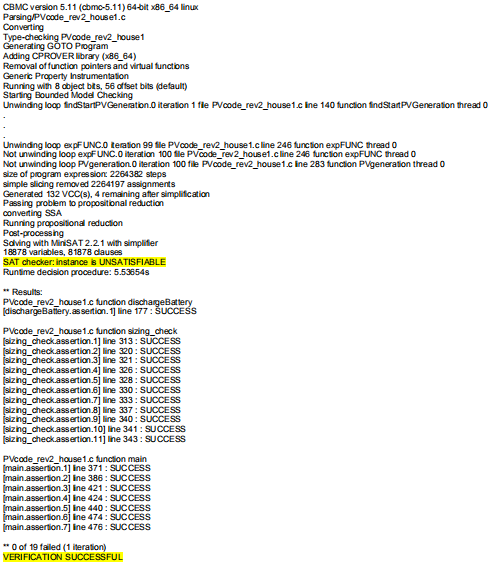
\includegraphics[width=0.8\textwidth]{cbmcverifh1.png}
\centering
\caption{Report generated by CBMC after validation of House 1.}
\label{fig:cbmcverifhouse1}
\end{figure}

However the 1,200 W PV system (house 5) failed (SAT) in line 337 of the code; with the same counterexample presented by ESBMC. This verification took less than 1 s to be performed as well. Fig.~\ref{fig:cbmcverifhouse5} shows the (edited) report produced, with the highlights about the flaw found: the minimum controller current needed to the PV systems is not compatible with the chosen controller of the sized system. The report file generated contained 217 lines and was 13 kB long.

\begin{figure}[h]
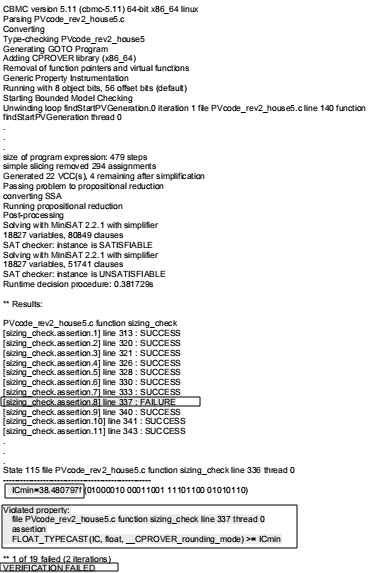
\includegraphics[width=0.7\textwidth]{cbmcverifh5.png}
\centering
\caption{Report generated by CBMC after validation of House 5.}
\label{fig:cbmcverifhouse5}
\end{figure}


\subsection{CPAchecker}

Finally, the CPAchecker tool presented some different results. Even using two different configuration possibilities, as described in Section~\ref{sec:setup}, the verification engine presented an UNKNOWN result for all the 700 W systems. This is because the \textit{time out} limit was reached, i.e., after 4 hours of execution the tool was unable to decide if the verification was SAT or UNSAT. 

Figure here CPA house 1

However, when verifying the 1,200 W PV system, the tool presented a SAT message equal to the other engines. 

Figure here CPA house 5


\subsection{HOMER Pro Environment}
\label{sec:homerenviron}

Screens and comments about the simulation tool.
1) If you want to simulate a particular capacity for PV and battery, you can use the search space instead of HOMER Optimizer for sizing. You can either aggregate all the 3 PV panels together as a single PV component or add 3 PV components to represent the series configuration. For the batteries, you will have to find the equivalent capacity of the series and parallel configuration since HOMER considers only one battery component per simulation even if you add multiple battery components in the schematic.
2) You cannot set the autonomy of the batteries as HOMER controller will decide when it is economical to discharge the batteries during the simulation year.

The same five case studies were evaluated by HOMER Pro (RQ2). The simulation results showed that the project restrictions were met by four 700 W PV systems (house 1, 2, 3 and 4), without any indication of sizing error or even performance related issues. All the simulations took less than 5 seconds (each) to be performed by HOMER Pro. Fig. \ref{fig:homerscreen1} shows one of the screens presented by HOMER Pro software, specifically to house 1.

\begin{figure}[h]
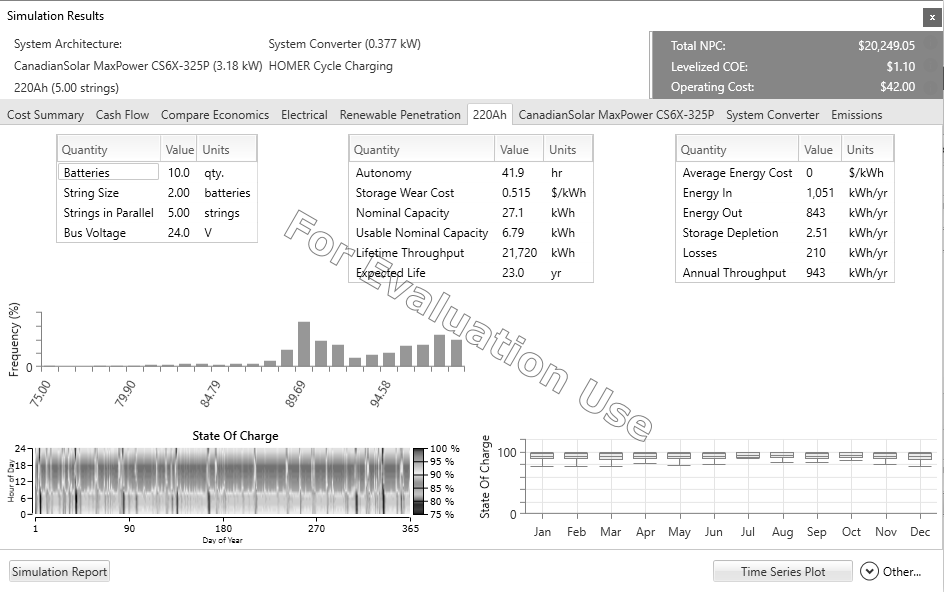
\includegraphics[width=0.8\textwidth]{homer.png}
\centering
\caption{HOMER simulation screen.}
\label{fig:homerscreen1}
\end{figure}

The case study that was not possible to simulate was the 1,200 W (house 5). The reason is based on the fact that HOMER Pro do not allow to set up a battery autonomy; therefore, it was was not possible to obtain any indication about the failures of this specifically PV system with simulation (RQ2).  


%
%Note that a PV design always uses daily average values of sun hours to each site, with impact in the PV components. Those hours are based on historical data and, in field, it is not unusual to find days where that number of hours was not reached due to weather conditions. The season has impact since the case studies are from the rain forest, where clouds are always present. As a result, the identified flaws in houses 1, 2, 3, and 4, are justified once again.
%
%We have evaluated five case studies in total using the HOMER Pro tool and our automated verification tool. Related to the HOMER Pro, the simulation, based on NASA data from the deployed systems (temperature and solar irradiance), shows that the restrictions were met by four 700 W PV systems (house 1, 2, 3 and 4), without any indication of sizing error or even performance. The case study that was unsuccessful during simulation was the 1,200 W (house 5); however, without any indication about the failures of this PV system. All the simulations took less than 5 seconds (each) to be performed.
%
%However, related to the results of the automated verification: (a) the 1,200 W PV system (house 5) failed during the sizing check. The number of panels was \textit{incorrect}; in particular, the counterexample provided by our verification method indicated 3 panels in parallel and the sized project has 2 in series and 2 in parallel. That verification took 63.3 hours to be performed. Surveying the owner of the 1,200 W system it was identified that, in fact, the system mostly of the time do not met the battery autonomy (mainly when all the loads are turned on). That behavior is expected because the system was purchased as an off-the-shelf solution and not as a specific design for the electrical charges of the house; (b) Related to the four 700 W PV systems, just one verification finished its analysis (house 1) considering the time-out of 432 h of computing. The sizing check was successful during automated verification, but there was found flaw related with the battery autonomy, when SOC reached levels below of 75\%. The automated verification identified the flaw right after the first night-discharge cycle, before the solar system start to recharge the batteries. The proposed tool took 409.3 hours to find this error at house 1. This possible flaw was confirmed with the dweller that uses the system: at least once or twice a mouth is usual the system to turn off, normally during raining days or with more clouds in the sky, and after the sun rises the system returns to normal operation. Related to houses 2, 3 and 4, it was considered that the automated verification had a time-out condition, with no conclusive results.

\subsection{Comparing Automated Verification and Simulation Results with Real PV Systems}

There were no divergence of results for the houses 1, 2, 3 and 4 w.r.t. of proposed approach, it is evident that the information collected from the dwellers and from the monitoring systems indicate that the proposed approach provides the correct evaluation of the PV system, thus answering RQ2. House 5 presented flaws from all tools (automated verified or simulation); however, only automated verification approaches indicated which design error was responsible for the flaw (charge controller specification), further answering RQ2.

In order to validate the possible flaw from house 5, it was surveyed the owner of the 1,200 W system. It was identified that, in fact, the system does not meet the battery autonomy when all loads are turned on, and this was double checked with the monitoring system from the charge controller, which showed that the maximum power or surge power were not exceeded, thus affirming RQ1; this behavior is expected since the system was purchased as an off-the-shelf solution and not as a customized design for the electrical charges of the house. The same process of validation was done to the houses 1, 2, 3 and 4, which use the 700 W PV systems: from July of 2018 to March 2019, a monthly visiting was performed to apply surveys to the dwellers and to collect data from a local monitoring system: not every month were reported some energy interruption of the PV systems. However, even when one interruption is reported in a month, this represents around 3.33\% of interruption for the entire period ($1/30$), which indicates 96.97\% of availability of the PV system ($96.67\% = 100\%-3.33\%$) 
and it is in accordance to what was described in Section~\ref{sec:availability}, because the type of electrical load of the houses is not critical; this situation is considered an energy interruption, but is not considered a system flaw, further affirming RQ1.

%\begin{figure}[h]
%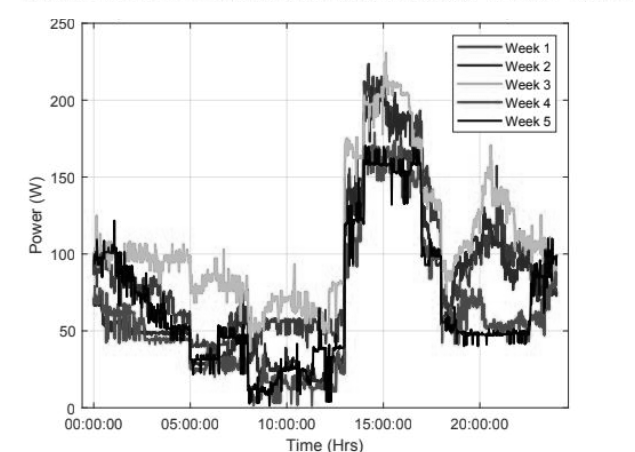
\includegraphics[width=0.65\textwidth]{loadcurve.png}
%\centering
%\caption{Five weeks monitored load curve from House 1.}
%\label{fig:loadcurve}
%\end{figure}
%
%\subsection{Experimental results}
%\label{sec:results}
%---------------------------------------------------
\section{Threats to Validity}
%---------------------------------------------------

At this Chapter, it was reported a favorable assessment of the proposed method. % over a diverse set of real-world benchmarks. 
Nevertheless, we have also identified five threats to the validity of the results that can further be assessed.

\textit{Model precision:} each component of the PV system is mathematically modeled. %, and the precision of the proposed method depends on the precision of that particular model. 
The adoption of more complex models, or even an evaluation in a PV laboratory to validate the model could add more reliability to the results.

\textit{Time step:} The run-time complexity of the proposed method is an issue; the time step of one hour can be further reduced to approximate the algorithm to the real-world scenario.

\textit{Case studies:} The case studies are performed only in one municipality. A more complete evaluation can be performed with more case studies.

\textit{Simulation Tool:} Only HOMER Pro was used. The inclusion of other specialized simulation tool or even a general simulation tool that uses the same mathematical model adopted by the automated verification could change the comparative.

\textit{Temperature and Solar Irradiance Data}: Information related to temperature and solar irradiance of each case study, independently of using simulation or formal verification, come from databases available online~\cite{Temperature, Irradiance}. However, considering that riverside communities do not have weather stations, the data used in the present study come from the closest municipality (Manaus in all case studies), where stations collect regularly those data. Therefore, the most accurate should be the use of weather stations in each location.

\section{Conclusion}

At this Chapter it was performed the comparative among verifiers with the proposed automated verification using model checking, which showed that 'incremental' ESBMC had the best overall performance. CBMC presented the same results, however with a worse time to result, and CPAchecker was not conclusive (house 1, house 2, house 3, and house 4) because the \textit{time out} was not enough to obtain some result.

A comparative with a specialized simulation tool was performed as well, however some limitations of the tool, mainly related to not allow battery autonomy setup, restricted the comparative between automated verification tools versus simulation tools.

Based on the fact that all case studies were deployed at the field, with regular visiting to perform interview with the dwellers, and with monitoring system in some of the houses (house 1, house 2, house 3, and house 4), it was possible to compare the computer obtained results with the real world employment of the stand-alone solar PV systems. The final conclusion was that the proposed tool is sound and with an acceptable performance. 

\chapter{Automated Formal Verification of Stand-Alone Solar PV Systems}
\label{chap:automatedverification}
In this chapter, we detail the methodology adopted to perform formal verification of stand-alone solar PV systems using formal methods, more specifically model checking. Diagrams, flowcharts, and algorithms support and explain the solutions. The experimentation, case studies, and results are also presented. In addition, the chapter contains a comparison with a specialized simulation tool, and also the use of different verifiers that evaluate performance by means of automated verification. Tables, commented reports, and graphic outputs are presented to aid  understanding.

Additionally, we present all assumptions and premises adopted, all of which support the results/conclusions, with direct impact on them. Usually, a premise is an unquestionable fact, however assumptions can be questioned. Unlike premises, assumptions are not explicit and need to be deciphered. With that in mind, we perform a detailed explanation of all assumptions over the course of the chapter.

It is important to emphasize that the theoretical basis of the subject presented in this chapter was discussed in chapter 2, ~\nameref{chap:background}. In addition, knowledge of the literature is essential to aid understanding.


\section{Methodology for Automated Verification of Solar PV Systems}

Fig.~\ref{fig:validation} illustrates how a stand-alone solar PV project can be validated, starting with the traditional techniques - manual, simulation, testing, only then including the proposed automatic verification that is detailed in this Section. 

Note that, on the one hand, although the input information is the same for all the techniques, automated validation is different in that it is possible to define the bound $k$ to restrict the space-design search. Among the possible inputs are: weather data at the location (temperature, solar irradiance, and insolation); system sizing information regarding specifications and configuration of PV panels, charge controller, inverter, batteries, DC bus  voltage; and requirements (battery autonomy, electric load demand, electric peak power demand, energy consumption, load curve, and AC voltage).

In contrast, the outputs are not equal: design-space coverage and the information presented as result. Design-space coverage was shown in chapter 2 (\nameref{chap:background}) to be the most complete when performed by automated verification, event using the bound $k$ to restrict the search, it not being necessary to unbound the system completely in order to discover a design flaw. Moreover, testing and simulation depend on the test vector used as input to evaluate the system.

With respect to the results presented, a project validated manually is just a piece of paper; simulation software produces success - fail information and can additionally present the optimized design if the system evaluated has some flaw, with graphics and reports; testing (whether laboratory or field) uses  measurement equipment and/or data from monitoring systems. Automated verification, as proposed in this thesis, presents success-fail information also, however the output is not graphic  (as will be shown), is summarized in reports with details about the variables and states of the project that cause a project flaw (in this case,  where a design flaw is detected).

\begin{figure}[h]
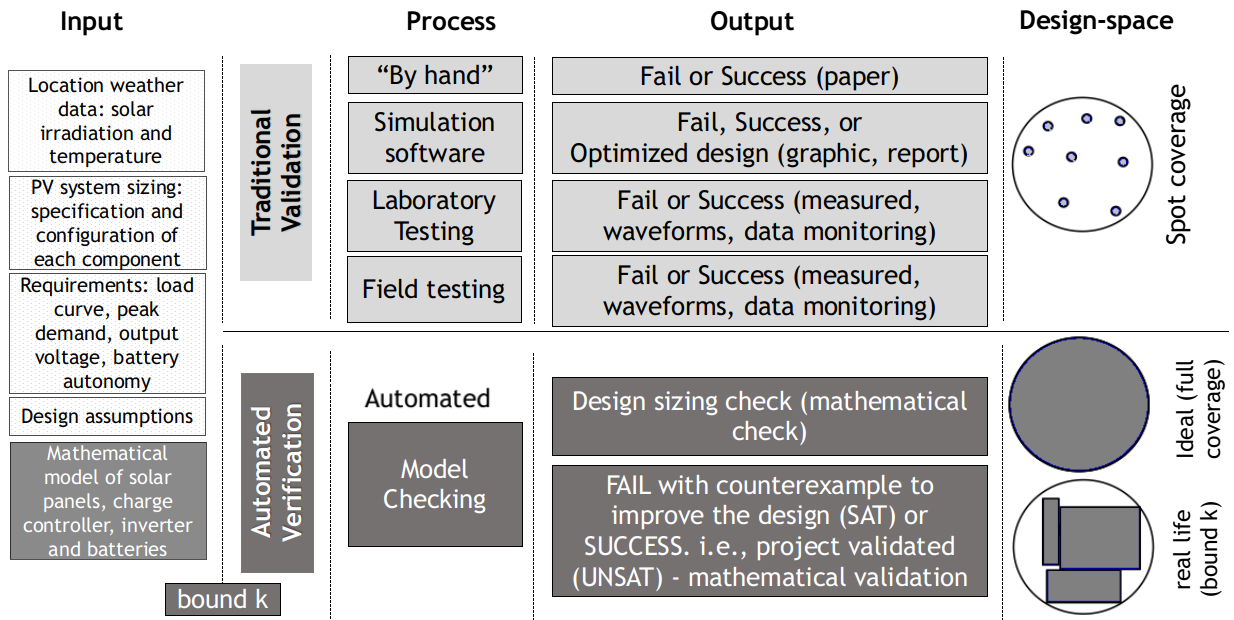
\includegraphics[width=1.0\textwidth]{PVprojectvalidation3g}
\centering
\caption{Project validation methods compared}
\label{fig:validation}
\end{figure}

Starting at this point, it will be shown how the proposed automated verification of stand-alone solar PV systems functions. 

The process begins with the conversion of a real PV system into a model. Fig. \ref{fig:systemverif} showed how a general system is converted to a model in order to be verified by model checking. Fig.~\ref{fig:systemverif4} is an adaptation of the general diagram, replacing the original system by a PV system and detailing the inputs, outputs, and requirements. 

It is important to bear in mind that the model checking process is the same whatever the system that is being validated; what is  important is to choose an accurate model, define the requirements/constraints, and get correct information from the system components, in order to achieve sound and effective validation.

\begin{figure}[h]
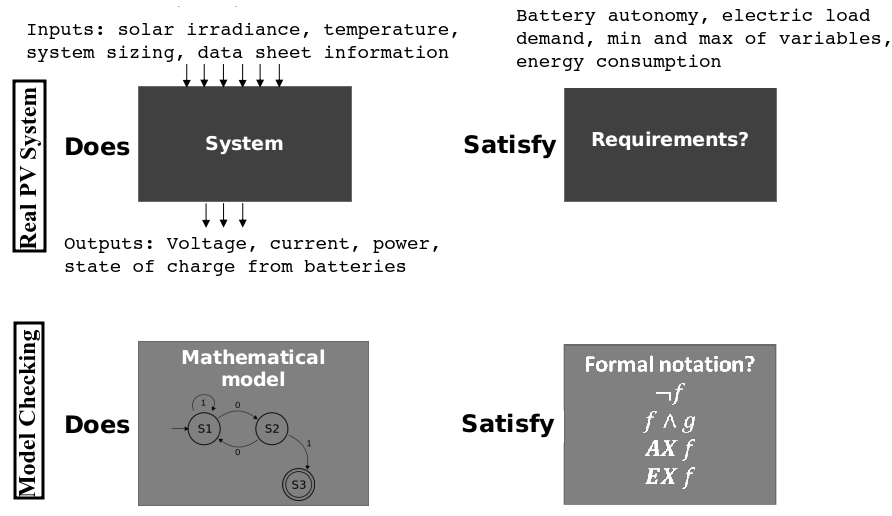
\includegraphics[width=0.8\textwidth]{systemverif4}
\centering
\caption{From real solar PV system verification to model checking. Source: adapted from \cite{Clarke2008}.}
\label{fig:systemverif4}
\end{figure}

The flowchart proposed for the automated verification method is illustrated in Fig.~\ref{fig:flowchartgeneral}. The three steps are the high level description of how the automated verification method can be used to validate solar PV systems.

\begin{figure}[h]
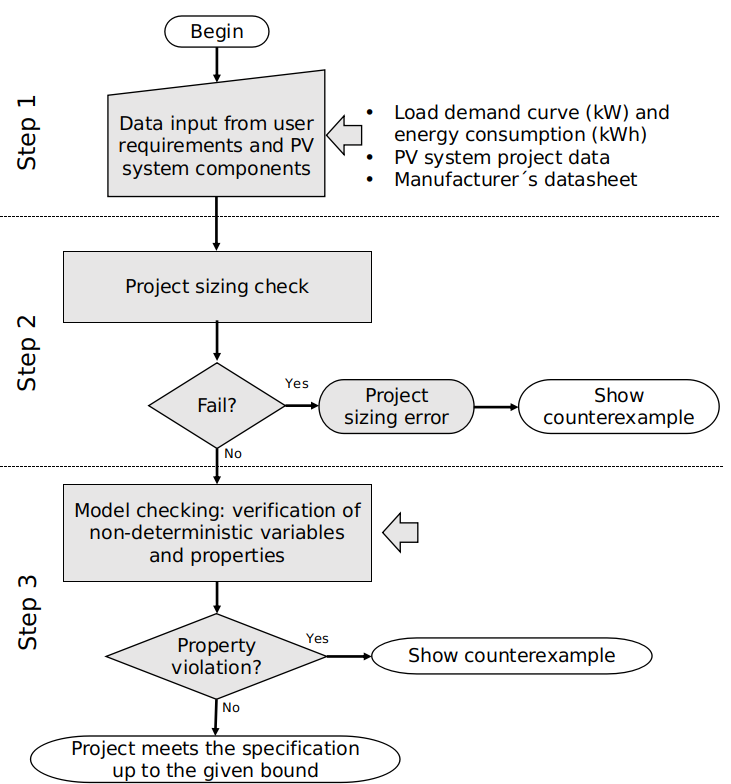
\includegraphics[width=0.6\textwidth]{flowchart_verification5.png}
\centering
\caption{Flowchart of the proposed automated verification of PV systems.}
\label{fig:flowchartgeneral}
\end{figure}

In \textbf{Step 1}, the PV input data %(e.g., load power demand and load energy consumption) 
and the formulae to check the sizing project, the mathematical model, the limits of the weather non-deterministic variables, are all written as an ANSI-C code~\cite{ANSI2018}. 

In \textbf{Step 2}, the sizing check of the PV system takes place: indicating if there is a sizing error before performing the automated verification of the system. This stage ensures that the system follows the standard project steps of the critical period method of sizing~\cite{Pinho}. 

\textbf{Assumption:} before the automated verification, which performs the verification of the intended system behavior, the sizing check of the system is performed. On the discover of an error, the process stops, showing the sizing error.

\textbf{Assumption:} The sizing check is performed using critical period criteria.

In \textbf{Step 3}, weather variables (e.g., solar irradiance and ambient temperature) will be systematically explored by our verification engine based on maximum and minimum values from the site where the PV system will be deployed. 
%As a consequence, all the formulae of the employed mathematical models will also be updated. 
In addition, depending on one of the desired properties of the system such as battery autonomy, energy availability, or even system power supply, our verification engine is able to indicate a failure if those properties are not met; in this particular case, it provides a diagnostic counterexample that shows in which conditions the property violation occurred. 
%; as the  state of charge of the batteries, load demand of power and the load consumption of energy if defined by the code
% (as reliability, performance, or safety)

%
%\textcolor{red}{In the following paragraph you should related the output of our verification engine with the description of the BMC SAT or UNSAR given above. For example, what does a failure mean? is it SAT?}
In short, the model checker will process the ANSI-C code with constraints ($C$) and properties ($P$) of the PV system, and the tool will automatically verify if the PV system requirements are met. If it returns a failure (i.e. SAT), then the tool provides a counterexample, i.e. a sequence of states that leads to the property violation; this information can be used as feedback to improve the PV system design. However, if the verification succeeds (i.e. UNSAT), there is no failure up to the bound $k$; therefore, the PV system will present its intended behavior up to the bound $k$.

%, i.e., our verification engine does not give any guarantee that there is no error in bound $k+1$ unless some induction method is employed~\cite{DBLP:journals/sttt/GadelhaIC17}.
%
%
%---------------------------------------------------------------------
% \subsection{The case studies and the Algorithm}
%---------------------------------------------------------------------
%
% 
%and as backup at night 
%
%The 700 W system: 3 x 325 W PV panels connected in series, controller of 150 V/35 A with a DC-bus of 24 V, 4 x 220 Ah batteries (2 in series and 2 in parallel arrangement), and inverter of 700 W. 
%
%And the 1,200 W PV system: 4 x 325 W connected in series PV panels, with controller of 150 V/35 A  in a DC-bus of 48 V, 4 batteries of 120 Ah connected in series, and a 1,200 W inverter.
%
%As demonstrated at this work, the performance of the system is highly dependent of solar irradiance and temperature, that are specific of the deployed local (latitude and longitude). 

Algorithm~\ref{alg:verification-algorithm} describes the equivalent pseudo-code. %Line 1 indicates a function call that performs the size checking of the each component of the PV system. %: using Equations \eqref{eq:NTPmin}, \eqref{eq:NTP}, \eqref{eq:NPSmin}, \eqref{eq:NPS}, \eqref{eq:NPP}, and \eqref{eq:NPPmin} to verify the PV panel; using \eqref{eq:Cbank}, \eqref{eq:Nbtotal}, and \eqref{eq:batcheck} to verify the batteries; using \eqref{eq:vcvsystem}, \eqref{eq:icmin}, and \eqref{eq:icicmin} to verify the charge controller; and using \eqref{eq:vindc}, \eqref{eq:voutac}, and \eqref{eq:invcheck} to verify the inverter. 
%The verification is carried out by the \textit{assert} macro from the ANSI-C programming language to encode each equation of sizing check. The argument to the \textit{assert} statement must be \textit{true} if the system specification is met; otherwise, the program aborts and prints a counterexample indicating a property violation. If there is no property violation, then the verification algorithm continues and 
In order to reduce the computational effort of the algorithm,
% caused by the state explosion inherent of the technique, 
every 24 h-day was considered as a time-step of 1 hour, and it was split into two parts: (a) one where PV generation is possible, during daylight, with a duration in hours depending on each site (but dependent on the sun and weather conditions); and (b) one that includes the rest of the day (with no PV generation), when the batteries are required to supply energy to the house.

\textbf{Assumption:} The day is divided into two parts (representing presence or absence of PV generation, based on historical data from the location), considering average temperature and solar irradiance (for every hour of the day) and  annual insolation (per day).

Lines 1 carries information from the location where the PV system will be/was deployed. We use the average annual minimum and maximum, both for temperature ($T$) and solar irradiance ($G$), hour by hour, from~\cite{Temperature}, and ~\cite{Irradiance}.

\textbf{Premise:} Temperature, solar irradiance, and insolation data is available pertaining to the location where the solar PV system will be used.

Line 2 represents all the information that derives from the PV sizing and from the equipment manufacturer's data: PV, battery, inverter and charge controller specification and data. This item also includes information from the house's load curve.

\textbf{Premise:} The data sheet of every element of the solar PV system to be validated is available.

\textbf{Premise:} The detailed, sized project of the PV system is necessary in order to perform the validation (list of equipment and configuration, including voltage, current and how they are connected).

\textbf{Assumption:} The load curve of every house must be estimated or measured. Moreover, the time step is 1 hour, and seasonality is not considered, i.e. the load curve is the same for the entire year.

The first automated verification is the sizing check (line 3), if an error is found then the algorithm stops. In order to perform the sizing check, the algorithm uses Equations \eqref{eq:NTPmin}, \eqref{eq:NPSmin} and \eqref{eq:NPPmin} to verify the PV panel, Equations \eqref{eq:Nbtotal}, and \eqref{eq:batcheck} to verify the batteries, Equations \eqref{eq:vcvsystem}, \eqref{eq:icmin} and \eqref{eq:icicmin} to verify the charge controller; and Equations \eqref{eq:vindc}, \eqref{eq:voutac} and \eqref{eq:invcheck} to verify the inverter.

Then, if no sizing design flaw is found, two functions, called at lines 4 and 5, are responsible for discovering at which hour PV generation starts and when it stops. These functions receive this information from the array inputted to the Algorithm with the solar irradiance values.

The batteries are assumed to be charged, i.e. with SOC of 100\% (line 6).

\textbf{Assumption:} Batteries are considered charged at the start of project validation.

The first for-loop at line 7 controls how many 24 hours cycleswill be performed by the Algorithm.  And the for-loop from lines 8 to 11 is responsible for discharging the battery (according the load curve) and verifying the state of charge of the battery, hourly, from the first hour of the day after the sun sets to the next day before the sun rises (without PV generation). Then, at the next for-loop, from line 12 to 29, verification is performed where there is solar irradiance and the whole PV system works. The Algorithm generates information hourly related to average temperature ($T$) and solar irradiance ($G$), using non-deterministic variables from the model checker to explore all possible states and the \textit{assume} macro to constrain the non-deterministic values using a given range (lines 15 and 16). 
%and irradiance varies from 0 W/m$^{2}$ to 852 W/m$^{2}$ (with minimum of 274 W/m$^{2}$ during the daytime, when there is sunlight). 
%there is PV generation only between 8:00 h and 16:00 h every day, 
%with zero electric energy generation from 18:00 h to 6:00 h of the next day; and with insignificant generation from 6:00 h to 8:00 h, and from 16:00 h to 18:00 h of the same day. 

After that, the model of the PV generator is used in the function call of line 17, to produce the voltage and current considering the states of $G$ and $T$. With respect to every hour considered, the conditional \textit{if-elseif-endif} statements from lines 18, 20, 22, 24 and 26, will imitate the charge controller's work, as depicted in Table~\ref{table:controller} of Section~\ref{sec:controller}, performing the charge or discharge of batteries according to the value of the different variables: if there is PV generation, the updated battery state of charge, the house's load and the PV system set-up information.

At the end of the last for-loop, the state of the batteries is verified again (line 27) and the hour is adjusted to the next loop (line 28).

Nevertheless, if the verification engine does not fail, we can conclude that the PV system does not need further corrections up to the given bound $k$.
%
%\textcolor{red}{this sentence is unclear... After this process is started the battery autonomy verification, from line 31}. \textcolor{red}{this sentence is unclear... Based on the fact that won't be PV generation after a given time of the day, the algorithm will only discharge the batteries until a new charging process (at the next day) to start.} \textcolor{red}{what do you mean by The formal verification is guaranteed?...  The formal verification is guaranteed by  macro to specific variables of the model, according lines 27 and 35.}
% and the non-deterministic variables $G$ and $T$ are considered during the formal verification of the system, otherwise, during the other two periods, there is no PV generation and just the power consumption from the backup batteries. 
%Within this 8h-period, $G$ and $T$ are automated verified with different values every one hour.
%, and change their value every 1 h according with the algorithm created using the technique.
 \begin{algorithm}
 \caption{Model checking algorithm for validation of stand-alone PV systems}
 \begin{algorithmic}[1]
 \begin{scriptsize}
 \renewcommand{\algorithmicrequire}{\textbf{Input:}}
 \renewcommand{\algorithmicensure}{\textbf{Output:}}
 \REQUIRE mathematical model (PV, batteries, inverter, charge controller), weather data (temperature, solar irradiance), system sizing details, design requirements (load curve, peak demand, output voltage, battery autonomy), design assumptions (system availability, battery state of charge, 1-hour step of validation)
 \ENSURE design sizing check; FAIL with counterexample to improve the design; SUCCESS, saying that the project has no flaws
  \STATE $declare \, min \, and \, max \, solar \, irradiance[24h], \, and \, temperature[24h]$\\
  \STATE $declare \, case \, studies \, details: \, sizing \, and \, manufacturers \, data $ \\
  \STATE $sizing \_ check()$ \\
  \STATE $startPVgeneration \leftarrow findStartPVgeneration()$ \\
  \STATE $endPVgeneration \leftarrow findEndPVgeneration()$ \\
  \STATE $SOC \leftarrow 100\%$ \\
%  \COMMENT {Starting with the PV generation time}
% \\ 
%\textit{LOOP Process}
 \FOR {$1st \, 24h \, loop$ to $Nth \, 24h \, loop$}
  \FOR {$endPVgeneration+1$ to $startPVgeneration-1$}
	  \STATE $dischargeBattery \, in \, 1h()$ \\
%	  \STATE $autonomyCount \leftarrow autonomyCount+1$ \\
	  \STATE $assert (SOC \geq SOC \_ min)$ \\
%	  \STATE $battery \, autonomy \, verification()$ \\
  \ENDFOR
  \FOR {$startPVgeneration$ to $endPVgeneration$}
    \STATE $G \leftarrow nondet \_ uint(\,)$ \COMMENT {$G$ is non-deterministic variable}
    \STATE $T \leftarrow nondet \_ uint(\,)$ \COMMENT {$T$ is non-deterministic variable}
    \STATE assume ($Gmin \leq G \leq Gmax$) \COMMENT {restricting $G$ values}
    \STATE assume ($Tmin \leq T \leq Tmax$) \COMMENT {restricting $T$ values}
    \STATE $Imax, Vmax \leftarrow PVgenerationMODEL (G,T)$ \\
    \COMMENT {If-then-else sequence to imitate charge controller work}
    \IF {($battery \, is \, empty$) AND ($PV \, is \, generating$)}
      \STATE $chargeBattery \, in \, 1h()$ \COMMENT {PV feed the house}
    \ELSIF {($battery \, is \, empty$) AND NOT($PV \, is \, generating$)}
      \STATE FAIL with assert macro \COMMENT {Battery is empty and there is not PV generation}
    \ELSIF {NOT($battery \, is \, empty$) AND ($PV \, is \, generating$)}
      \STATE stop battery charge \COMMENT {PV feed the house}
    \ELSIF {NOT($battery \, is \, empty$) AND NOT($PV \, is \, generating$)}
      \STATE $dischargeBattery \, in \, 1h()$ \COMMENT {Battery feed the house}
    \ENDIF
    \STATE $assert (SOC \geq SOC \_ min)$ \\
    \STATE $hour \leftarrow hour+1$ \\
   \ENDFOR
  \ENDFOR
 \RETURN $(\,)$ 
  \end{scriptsize}
 \end{algorithmic} 
 \label{alg:verification-algorithm}
 \end{algorithm}

%\subsubsection{Assumptions and Premises} 
%

\section{General Assumptions}
\label{sec:assumptions}

In order to be clear, we now provide a list of the assumptions adopted by the scientific automated verification methods developed in this thesis.

The code in ANSI-C, was created to perform both methods, automated verification and automated synthesis, regardless of the verifier used. This means that: 

\begin{itemize}
\item The `\# include' preprocessor directive is not used, despite being very common in the C language, which allows the use of C language libraries, including the mathematical one;
\item In the absence of the `\# include' directive, it was necessary to create specific mathematical functions at the proposed code in order to calculate the exponential `$exp(x)$' or $e^{x}$, and natural logarithm `$log(x)$' functions, used for the solar PV model;
\item There is no `\# define' preprocessor directive. Therefore, global variables were used to replace it;
\item The macro `assert (expression);' must be replaced by `if (!expression) \{ \_ \_ VERIFIER\_ error();\}';
\item The macro `assume (expression);' must be replaced by `\_ \_ VERIFIER\_ assume(expression);';
\item It is not possible to use the \# if, \# else, \# elif, \# endif or \# ifdef, \# ifndef commands.
\end{itemize}

Regarding the automated verification scientific method:

\begin{itemize}
\item A value of bound $k$ was used to restrict the design-space and improve performance. The choice of value was empirical, following tests with the code;
\item All the PV system model, user requirements, assumptions, and technical information from the PV system equipment are written as an ANSI-C code.
\end{itemize}

Of the off-the-shelf simulation tools, only HOMER Pro and Hybrid2 perform off-grid system with battery backup analysis. Additionally, HOMER and RETScreen include economic analysis or even optimization-sensitive analysis; however RETScreen does not have the capacity for stand-alone solar PV system analysis. Therefore, in this study, HOMER Pro will be the only simulation tool used to compare with our method.  

For all case studies, the minimum battery state of charge was defined at $75$\%, and the efficiency of $86$\%, which is common to lead-acid batteries (adopted as standard here), and the AC voltage from the inverter at $127$ V (Brazilian standard). According with the evaluated local of the PV systems installation, the considered insolation for the worst month is $3.8 kWh/m^{2}$ per day.


\section{Description of the Case Studies}
%------------------------------------------

%We have performed five case studies to evaluate our proposed verification method: (a) four PV systems (three in series 325W PV panels, four 220 Ah batteries in a configuration with two series and two parallel with 48h autonomy, 700 W inverter with peak power of 1,600W, charge controller with MPPT with 35A/150V of capacity) deployed in four different houses in an indigenous community (GPS coordinates 2$^{o}$44'50.0"S 60$^{o}$25'47.8"W) situated nearby Manaus (Brazil), with each house having a different power demand (house 1 = 253 W, house 2 = 263 W, house 3 = 283 W, and house 4 = 501 W); and (b) one case concerning a system deployed as an individual system in Manaus (GPS coordinates 3$^{o}$4'20.208"S 60$^{o}$0'30.168"W), supporting 915 W of the house's load (house 5 with four 325W PV panels in a configuration two series and two parallel, four 120Ah batteries in series and autonomy of just 6 h, 1,200 W inverter with surge of 1,600 W, charge controller with MPPT of 150V/35A). 
Five case studies evaluated the proposed approach, as described in Table~\ref{tab2}. %Furthermore, three start-of-art verification tools, as described in Section~\ref{sec:AutomatedVerification} (ESBMC, CBMC, and CPAchecker), and HOMER Pro simulation tool were used to compare the approach effectiveness and efficiency.
These case studies were defined based on the usual electrical load found in riverside communities in the State of Amazonas,  Brazil~\cite{TrindadeCordeiro19, Agrener2013}.

It is important to mention that the load curve represents an array of $24$ integer numbers, one for each hour of the day (instant power in Watts) and it was estimated after visits to the communities and a survey applied in June $2017$, before the houses were electrified.

\begin{table}
\caption{Case studies: stand-alone solar PV systems.}\label{tab2}
\begin{scriptsize}
\begin{tabular}{c|c|c|c|c|c}
\hline
\hline
Item & House 1 & House 2 & House 3 & House 4 & House 5\\
\hline
\hline
PV Panels &  \multicolumn{4}{|c|}{3$\times$325 W: (3S)} & 4$\times$325 W: (2S-2P) \\
\hline
Batteries & \multicolumn{4}{|c|}{\makecell{4$\times$220 Ah: (2S-2P)\\ autonomy: 48 h}} & \makecell{4$\times$120 Ah: (4S)\\ autonomy: 6 h}\\
\hline
Charge Controller & \multicolumn{5}{c}{With MPPT of 150 V/35 A}\\
\hline
Inverter & \multicolumn{4}{c}{700 W, surge: 1,600 W} & 1,200 W, surge: 1,600 W\\
\hline
Load power peak (W)& 342  & 253  & 263 & 322 & 814 \\
\hline
Load power surge (W)& 342 & 722 & 732 & 896 & 980\\
\hline
Load curve (W) & \multicolumn{5}{l}{\makecell{House 1: 118-118-118-46-46-46-95-95-170-170-296-242-242-95-95-95-95-95-342-288-288-288-288-118\\House 2: 136-136-136-136-136-136-67-67-184-184-184-184-184-67-67-67-67-67-253-253-253-253-253-136\\House 3: 113-113-113-113-113-113-67-67-217-97-97-97-97-97-97-97-97-97-263-113-113-113-113-113\\House 4: 207-207-207-135-135-135-66-66-161-161-233-253-248-66-66-66-66-66-302-317-322-302-302-207\\House 5: 45-16-16-16-16-16-0-0-0-72-72-222-150-150-0-0-72-72-814-814-814-742-742-16}}\\
\hline
\makecell{Consumption\\ (kWh/day)}& 3.9 & 3.6 & 2.5 & 4.3 & 4.88\\
\hline
GPS Coordinates & \multicolumn{4}{|c|}{\makecell{2$^{o}$44'50.0"S 60$^{o}$25'47.8"W\\}} & \makecell{3$^{o}$4'20.208"S \\60$^{o}$0'30.168"W}\\
\hline
Details & \multicolumn{4}{|c|}{\makecell{Riverside indigenous community\\Rural Area of Manaus - Brazil}} & \makecell{Urban house \\Manaus-Amazonas-Brazil}\\
\hline
\hline
\end{tabular}
Caption: (S): Series; (P): Parallel.
\end{scriptsize}
\end{table}

%------------------------------------------
\section{Objectives and Setup}
\label{sec:setup}
%------------------------------------------

The experimental evaluation aims to answer two experimental questions:
%
\begin{enumerate}
\item[EQ1] \textbf{(soundness)} Does the automated verification approach provide correct results?
\item[EQ2] \textbf{(performance)} How do the verifiers compare to each other and to a commercial simulation tool?
\end{enumerate}

%In order to evaluate the proposed verification method and its performance, we have considered five case studies, three verification engines in different configurations, and also compared the results to the HOMER Pro tool. All the experiments were performed with a time out of 14,400 seconds. %Every dweller, who owns a PV system, was interviewed 
%
All experiments were conducted on an otherwise idle Intel Xeon CPU E5-4617 (8-cores) with 2.90 GHz and 64 GB RAM, running Ubuntu 16.04 LTS 64-bits. The setup of HOMER Pro v3.13.1 was an Intel Core i5-4210 (4-cores), with 1.7 GHz and 4 GB RAM, running Windows 10. The experiments were performed with a time out of 240 minutes.

The verification engine ESBMC, version v6.0.0 was used with the SMT solver Boolector version 3.0.1~\cite{Brummayer}\footnote{Command-line: \$ esbmc filename.c -\phantom{}-no-bounds-check -\phantom{}-no-pointer-check -\phantom{}-unwind 100 -\phantom{}-boolector}; and an alternative ESBMC v6.0.0 was used with the 'incremental SMT' mode\footnote{Command-line: \$ esbmc filename.c -\phantom{}-no-bounds-check -\phantom{}-no-pointer-check -\phantom{}-unwind 100 -\phantom{}-smt-during-symex -\phantom{}-smt-symex-guard -\phantom{}-z3} enabled; with SMT solver Z3 version 4.7.1~\cite{DeMoura}. % with the goal of reducing memory usage.

The verification engine CBMC 5.11 and MiniSat 2.2.1 were used in the comparison~\cite{Kroening}\footnote{Command-line: \$ cbmc filename.c -\phantom{}-unwind 100 -\phantom{}-trace}.
 
The verification engine CPAchecker 1.8 was used in a configuration of bound model checking\footnote{Command-line: \$ scripts/cpa.sh -heap 64000m -stack 10240k -config config/bmc-incremental.properties -spec config/specification/sv-comp-reachability.spc -benchmark filename.c}, with the SMT solver MathSAT version 5.5.3~\cite{mathsat5}. An alternative CPAchecker configuration was also tried, using the BMC k-induction option, but the results show no improvement in performance or soundness (so it is not reported here).

%\section{Verifiers Environment}
%\label{sec:verifenviron}

%------------------------------------------
\section{Experimental Results and Discussion}
\label{sec:results_indeed}
%------------------------------------------

This Section presents the results, with commented outputs produced by every tool, mainly related to the reports (CBMC and ESBMC) and some graphic resources (CPAchecker and ESBMC).

%\textcolor{red}{We should answer the two% research questions here... please take a look at https://ssvlab.github.io/lucasccordeiro/papers/cav2017.pdf to check how you can answer.}
%\begin{enumerate}
%\item[RQ1] \textbf{(soundness)} Does our approach provide correct results?
%\item[RQ2] \textbf{(performance)} How does our approach compare against other existing tools?
%
Table~\ref{cases} summarizes the results. The times reported in Table~\ref{cases} answer EQ2. 
Note that an UNKNOWN result from the proposed verification engines does not mean that a failure was found nor that the verification was successful: it indicates that the verification engine led to an \textit{out of memory} situation and the design-state explosion was a issue during the run-time. It worth to mention that none of the verifiers and solvers reached the \textit{time out} limit during the experimental evaluation.

%HOMER Pro result: the $1,200$W was the only one that was proved to not meet the requirement of battery autonomy; all the 700W systems had no indication of flaws during simulation. The simulation took less than five seconds to be performed on each case study.
%
\begin{table}
\centering
\caption{Summary of the case-studies comparative and the automated tools.}\label{cases}
\begin{scriptsize}
\begin{tabular}{c|c|c|c|c}
\hline
\hline
\multicolumn{5}{c}{Model Checker (SAT/UNSAT: time, message, and used memory)}\\
\hline
Case &  \makecell{ESBMC 6.0.0\\(Boolector 3.0.1)} & \makecell {ESBMC 6.0.0\\(Z3 4.7.1)} & \makecell{CBMC 5.11\\(MiniSat 2.2.1)} & \makecell{CPAchecker 1.8\\(MathSAT 5.5.3)}\\
\hline
\hline
House 1 &  \makecell{Out of memory \\(UNKNOWN)\\$\geq$ 64 GB} & \makecell{$\leq$ 1 sec \\(SAT) \\ 44 MB} & \makecell{Out of memory \\(UNKNOWN)\\$\geq$ 64 GB} & \makecell{4.36 s \\ (SAT) \\ 173 MB}\\
\hline
House 2 &  \makecell{Out of memory \\(UNKNOWN)\\$\geq$ 64 GB} & \makecell{$\leq$ 1 sec \\(SAT)\\ 44 MB} & \makecell{Out of memory \\(UNKNOWN)\\$\geq$ 64 GB} & \makecell{4.34 s \\ (SAT)\\174 MB}\\
\hline
House 3 &  \makecell{Out of memory \\(UNKNOWN)\\$\geq$ 64 GB} & \makecell{$\leq$ 1 sec \\(SAT)\\ 45 MB} & \makecell{Out of memory \\(UNKNOWN)\\$\geq$ 64 GB} & \makecell{4.38 s \\ (SAT)\\ 174 MB}\\
\hline
House 4 &  \makecell{Out of memory \\(UNKNOWN)\\$\geq$ 64 GB} & \makecell{$\leq$ 1 sec \\(SAT)\\ 45 MB} & \makecell{Out of memory \\(UNKNOWN)\\$\geq$ 64 GB} & \makecell{4.46 s \\ (SAT)\\ 176 MB}\\
\hline
House 5 &  \makecell{Out of memory \\(UNKNOWN)\\$\geq$ 64 GB} & \makecell{$\leq$ 1 sec \\(SAT)\\ 45 MB} & \makecell{Out of memory \\(UNKNOWN)\\$\geq$ 64 GB} & \makecell{4.19 s \\ (SAT)\\ 174 MB}\\
\hline
\hline
\end{tabular}
\\Caption: (SAT): wrong sizing of PV panels (minimum total installed power not satisfied).
\end{scriptsize}
\end{table}

The description of the experimental results have been broken down into three parts, one for each verification engine: ESBMC, CBMC, and CPAchecker. 

\subsection{ESBMC}
\label{sec:ESBMCverification}

Two alternatives were tested with ESBMC: one with Boolector and the another with Z3. The 'incremental SMT' option, which uses less memory, can be performed with Z3 only since ESBMC does not support the 'incremental' mode with the Boolector solver yet. 

Using ESBMC with Boolector led to an 'out of memory' situation in all the case studies. This result was obtained in less than six minutes of execution, i.e. the $64$ GB of RAM were consumed by the verification engine and the processes were killed, thus leading to an UNKNOWN result returned by ESBMC as shown in the first column of Table~\ref{cases}. 

However, running the same version of ESBMC, using 'incremental SMT' solving with Z3, the experimentation results returned were conclusive (SAT) in all the case studies. Moreover, the flaw identified was the same for all cases: the sized total PV panels power was not enough to meet the design requirements of the system (energy and power load demand). Put it simple, the designed PV systems will fail when deployed at the field. Based on the fact that the tool stops when the first flaw is identified, the rest of the validation procedure was not even reached. Worth to mention that if we remove the PV panels validation from the tool, the next flaw identified during experimentation was the battery array sizing (not enough to meet the design requirements as well).

In the houses that use a $975$ W PV system (house $1$, house $2$, house $3$, and house $4$), ESBMC reached an error in all the four houses and the execution time took less than $01$ s. Fig.~\ref{fig:esbmcverifhouse1} shows the output report of the tool for house $1$, with the FAIL identified. The authors highlighted the result, which shows that the design flaw was found (SAT result or SUCCESS) within the bound $k$ of $100$, when a PV panels total power of $1,636.76$ W is expected and the sized system has only $975$ W. This flaw is related to Eq.~\eqref{eq:Pminpanel}.

\begin{figure}[h]
\fbox{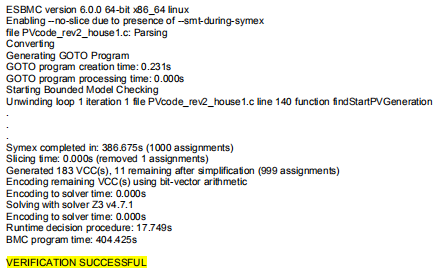
\includegraphics[width=1.0\textwidth]{esbmcverifh1.png}}
\centering
\caption{Report generated by ESBMC (Z3 solver) after validation of House 1.}
\label{fig:esbmcverifhouse1}
\end{figure}

Related to the $1,300$ W PV system (house $5$), the same fail occurred (SAT), thereby indicating that the system is \textit{incorrectly} sized. Fig.~\ref{fig:esbmcverifhouse5} shows the report generated by the tool, with highlights for the result, showing the incompatibility of the sized PV panels array of $1,300$ W and the minimum necessary of $2,048.05$W. This verification took less than $1$ s to perform, as indicated in the last line of Table~\ref{cases}.

\begin{figure}[h]
\fbox{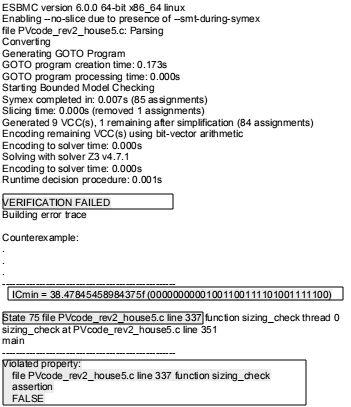
\includegraphics[width=1.0\textwidth]{esbmcverifh5.png}}
\centering
\caption{Report generated by ESBMC (Z3 solver) after validation of House 5.}
\label{fig:esbmcverifhouse5}
\end{figure}


\subsection{CBMC}

CBMC was unable to produce a SAT or UNSAT result. In less of the 25 minutes of code execution at the setup configuration, the verifier engine consumed all the available RAM memory and produced an UNKNOWN result, i.e the result was inconclusive for all houses. 


\subsection{CPAchecker}
%\label{sec:CPAresult1}

Finally, the CPAchecker tool presented some similar qualitative results but with different performance when compared with ESBMC (with Z3 solver). The verification engine presented an SAT result (a FAIL) for all the $975$ W systems (house $1$, house $2$, house $3$, and house $4$) and to $1,300$ W system.

Once again the problem of the minimum PV panels sizing expected was indicates as a flaw. The time to result was obtained in less than 5 seconds, around 4 seconds slower than ESBMC (with Z3); and the consumed memory by the CPAchecker was $3.86$ time bigger than ESBMC (with Z3).

Figure~\ref{fig:cpavalidh1} reproduces one of the text reports issued by CPAchecker. Unlike ESBMC and CBMC, CPAchecker produces many different reports, notably for log, statistical, and counterexample files. There is a HTML version of the counterexample which produces graphic output, not only text format.

\begin{figure}[h]
\fbox{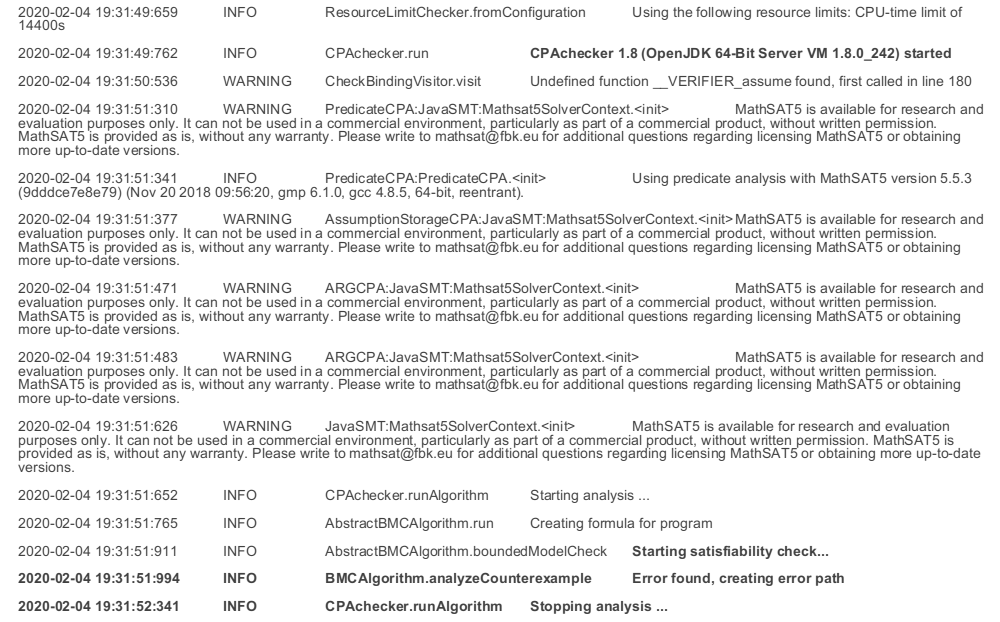
\includegraphics[width=1.0\textwidth]{CPA_verif_h1.png}}
\centering
\caption{CPAchecker text result for house 1 validation (file CPALog.txt).}
\label{fig:cpavalidh1}
\end{figure}

Figure~\ref{fig:cpavalidh5} shows the result for the $1,300$ W house, with highlights on the line that causes the fail and part of the CFA (control-flow automata, represented as a control-flow graph) diagram pointing to this fail.

\begin{figure}[h]
\fbox{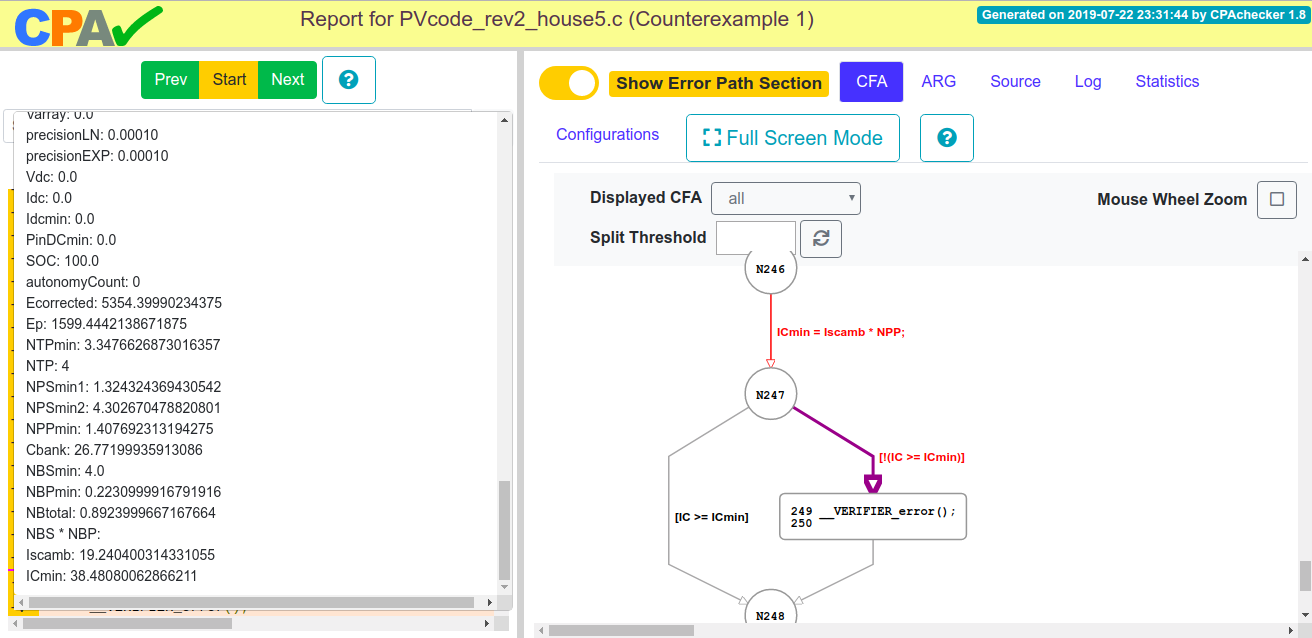
\includegraphics[width=1.0\textwidth]{CPA_verif_h5.png}}
\centering
\caption{CPAchecker graphic result for house 5 validation (file Counterexample.html).}
\label{fig:cpavalidh5}
\end{figure}


\subsection{HOMER Pro Specialized Simulation Tool}
\label{sec:homerenviron}

HOMER Pro is a powerful specialized electrical systems simulator, however even with the simulation characteristic, it performs optimization only when a given design is inputted to the schematic of the tool. This means that HOMER does not maintain the characteristic of the system under evaluation. It starts with the inputted information, but uses the optimization default set up to increase or decrease the characteristic of each component until the load is fulfilled by the electrical generation system, and at the lowest cost. 

Therefore, in order to perform a limited simulation and not exceed the values of each component (for example, the total power of the PV array under evaluation), the `search space' must be used for sizing instead of the `HOMER Optimizer'. This is done on the menu of each component inputted in the schematic of the tool. 

The PV panels and batteries: simulation of a particular capacity for PVs and batteris is possible using the `search space' for sizing instead of the `HOMER Optimizer'. It is possible either to aggregate all the PV panels as a single PV component, in which case, the search space must vary from 0 to 1, i.e. from the option without PV panels until it reaches the power inputted to the component in the HOMER schematic, or add each PV component to represent the series' configuration. For the batteries, it is necessary to find the equivalent capacity of the series and parallel configuration since HOMER considers only one battery component per simulation even if multiple battery components are added to the schematic.

Another drawback of HOMER Pro is the fact that the user cannot set battery autonomy, as the HOMER controller will decide when it is economical to discharge the batteries during the simulation year. It follows that simulation of battery autonomy cannot to be evaluated.

As part of the comparison proposed, four $975$ W PV systems (houses $1$, $2$, $3$ and $4$) were evaluated by HOMER Pro (EQ2). The simulation results showed that for each of the sized systems, HOMER Pro concluded that no viable solution was found with the components inputted in the schematic. Fig. \ref{fig:homersimuh2no} shows one of the screens presented by HOMER Pro software, specifically by house $2$.

\begin{figure}[h]
\fbox{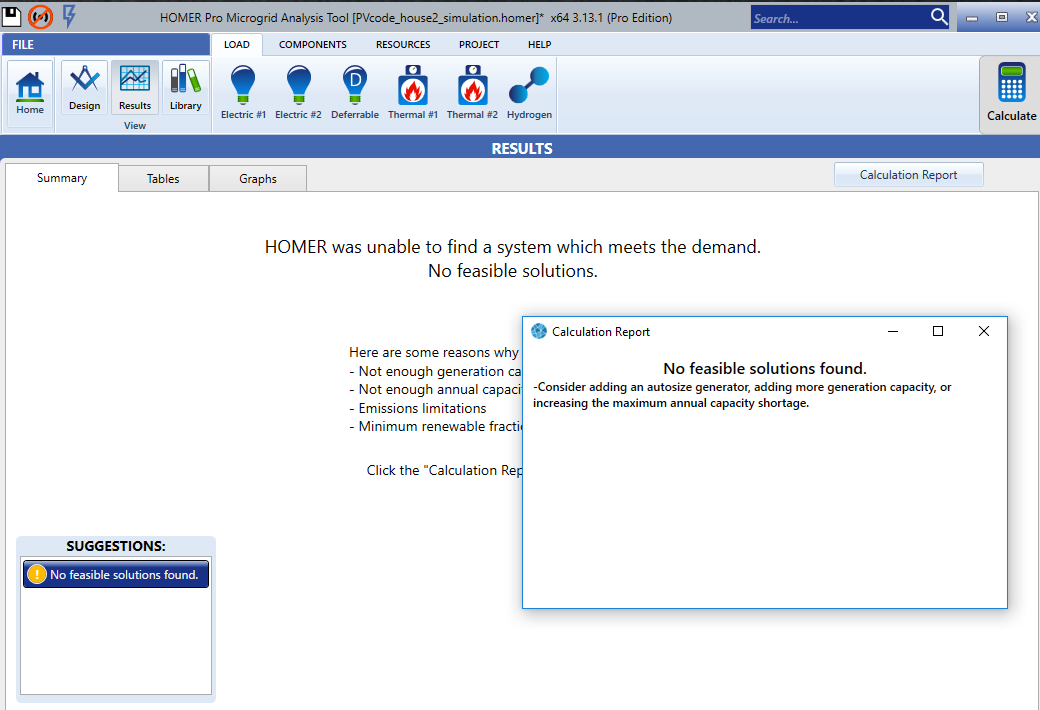
\includegraphics[width=1.0\textwidth]{homersimuh2no.png}}
\centering
\caption{HOMER simulation screen presented for house 2 with no feasible solution found.}
\label{fig:homersimuh2no}
\end{figure}

Moreover, in order to evaluate the problem associated with the lack of a viable solution, some empirical changes were made to the  project under evaluation. Fig.~\ref{fig:homersimuh2yes} shows that a configuration with higher battery capacity (3 strings of 2 batteries each, 2S-3P, of 220 Ah; instead of 2 strings of 2 batteries each as in the original sized system) can solve the problem of house 2. The same is true of the other three houses of $975 W$, when improved battery capacity is presented by HOMER Pro as an optimal solution. 

Further tests were performed in HOMER Pro. For example, to the case 1, that consumes $3.9$ kWh/day of energy: with the optimizer feature turned on, the total of PV panels minimum power expected to meet the load requirement was $2,530$ W. For the $3.6$ kWh/day of case 2, the PV panel solution indicated was $2,420$ W. For the $2.5$ kWh/day of case 3, the PV panel solution indicated was $1,590$ W. And, finally, for the $4.3$ kWh/day of case 4, the PV panel solution was $3,150$ W.

\begin{figure}[h]
\fbox{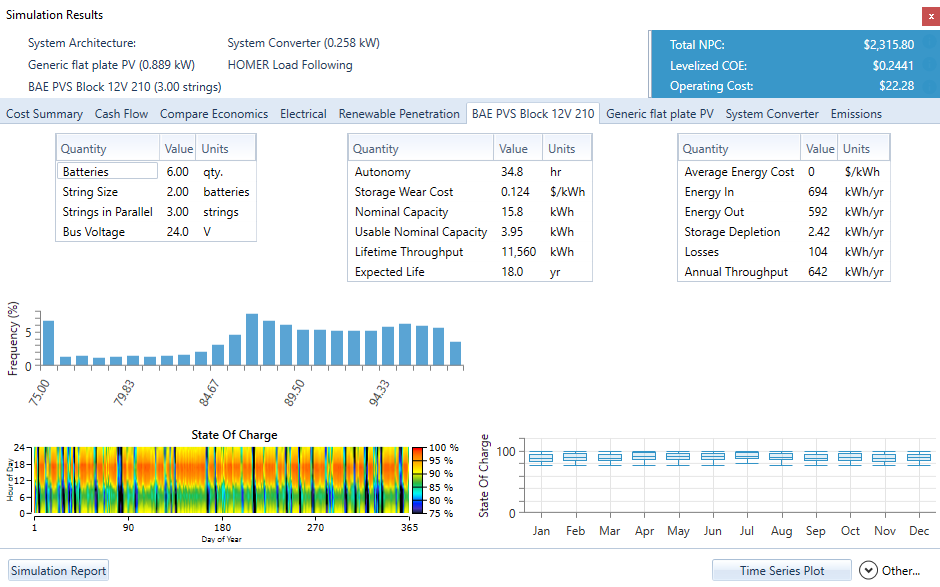
\includegraphics[width=1.0\textwidth]{homersimuh2yes.png}}
\centering
\caption{HOMER simulation screen presented for house 2 with viable solution.}
\label{fig:homersimuh2yes}
\end{figure}

The case study that was not possible to simulate was the $1,300$ W (house $5$). The reason is that HOMER Pro does not allow battery autonomy setup (because it always sizes and optimizes the electrical system in order to meet the load requirements for an entire year of simulation); therefore, it was not possible to obtain any indication about the failures of this specific PV system with simulation (EQ2).  

\subsection{Comparing Automated Verification and Simulation Results with Real PV Systems}

Results do not diverged for houses $1$, $2$, $3$, $4$, and $5$ with respect to the proposed approach: the automated evaluation shows there is project flaws, from the PV panels to the battery arrays sizing. Simulation demanded improvement of battery capacity (adding one more string of batteries to the system) and to the PV panels array (when the HOMER Pro tool was doing optimization of the original sized solution). 

In order to evaluate the validation results, it was necessary to consult the interviews conducted with the residents of the $975$ W deployed systems. From July $2018$ to March $2019$, surveys were applied to the residents on a monthly basis and data was collected from a local monitoring system: energy interruptions of the PV systems were not reported every month and, in some, cases, the maximum of 3 interruptions were reported. In one hand, when only one interruption is reported per month, this represents around $3.33$\% interruption for the entire period ($1/30$), which indicates $96.97$\% of availability of the PV system ($96.67\% = 100\%-3.33\%$). In other hand, when 3 interruptions are reported\footnote{Crossed information from interviews and collected data from the systems shows that the residents try to hide (or minimize) the interruption problems of the PV systems. Probably because they need of the system and they try not to emphasize this issue}, this means $10$\% of interruption, or $90$\% of availability. In accordance to what was described in Section~\ref{sec:availability}, the type of electrical load of the houses is not critical. Therefore any availability below of $95$\% is a sizing flaw, further affirming EQ1. Moreover, the proposed approach using automated verification provides the correct evaluation of the PV system, as the simulation did, thus answering EQ2.

The automated verification tools indicated flaws in house $5$ as well; and was not possible to get HOMER Pro evaluation because of the autonomy restriction, further answering EQ2.

In order to validate the possible flaw identified by the automated verification in house $5$, the owner of the $1,300$ W system was interviewed. From this it became clear that, in fact, the system does not meet the battery autonomy when all loads are turned on, and this was double-checked against the monitoring system of the charge controller, which showed that the maximum power or surge power was not exceeded. Even during the daylight, there is not enough energy produced by the solar PV panels to feed the loads, thus affirming EQ1; this behavior is to be expected since the system was purchased as an off-the-shelf solution and not as a customized design for the house's electrical charges. 

%\begin{figure}[h]
%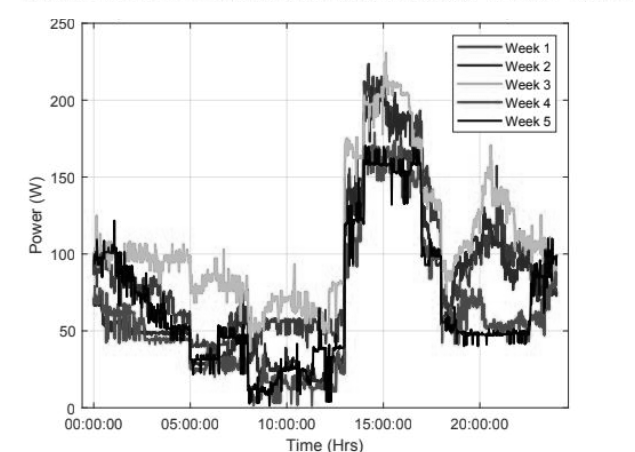
\includegraphics[width=0.65\textwidth]{loadcurve.png}
%\centering
%\caption{Five weeks monitored load curve from House 1.}
%\label{fig:loadcurve}
%\end{figure}
%
%\subsection{Experimental results}
%\label{sec:results}
%---------------------------------------------------
\section{Threats to Validity}
%---------------------------------------------------

This chapter presented a favorable assessment of the proposed method. % over a diverse set of real-world benchmarks. 
Nevertheless, it also identified six threats to the validity of the results that bear further assessment.

\textit{Model precision:} each component of the PV system is mathematically modeled. %, and the precision of the proposed method depends on the precision of that particular model. 
The adoption of more complex models, or even an evaluation in a PV laboratory to validate the model could add more reliability to the results.

\textit{Time step:} The run-time complexity of the proposed method is an issue; the time step of one hour could be further reduced to approximate the algorithm to the real-world scenario.

\textit{Case studies:} The case studies were conducted in only one municipality. A more complete evaluation can be done with more case studies.

\textit{Simulation tool:} Only HOMER Pro was used. The inclusion of other specialized simulation tools or even a general simulation tool that uses the same mathematical model adopted by the automated verification could change the comparison.

\textit{Temperature and solar irradiance data}: Information relating to the temperature and solar irradiance of each case study, whether it is using simulation or formal verification, comes from databases available online~\cite{Temperature, Irradiance}. However, in view of the fact that riverside communities do not have weather stations, the data used in the present study comes from the municipality closest (Manaus in all the case studies), where stations regularly collect the data. Nevertheless, accuracy recommends the use of weather stations in each location.

\textit{Energy consumption estimation}: All the PV size verification procedure start from the value of energy demanded from every house. However, this is a estimated value. Most recent information from field indicates that this value is overestimated and probably must be adjusted based on real data from a monitoring systems. The fact of the residents receive training to save energy is other issue that can reduce the total demanded energy from the PV systems. Therefore a most accurate validation can be performed when a real load curve is available for every case study.

\section{Conclusion}

This chapter showed in details how the state-of-the-art computer science method of automated verification was adapted to be used in stand-alone solar PV systems in order to validate their behavior. Moreover, it was possible to illustrate the comparative differences in how the proposed method and the traditional method of simulation work.

Detailed diagrams, flowcharts and algorithm with pseudo-code were presented in support of the proposed work and to aid the understanding. Additionally, the assumptions adopted in relation to the automated verification and simulation software were listed.

Furthermore, in this chapter verifiers with the proposed automated verification using model checking were compared, which demonstrated that 'incremental' ESBMC had the best overall performance. CBMC was not conclusive, presented out of memory issues in all cases. CPAchecker had similar quality results than ESBMC, but with a slower performance for all cases.

A comparison with a specialized simulation tool was also performed, although some of the tool's limitations, mainly related to not allowing battery autonomy setup.  The need of better PV panels and/or battery sizing by HOMER Pro and the verifier engines showed the flaws identified by the tools.

Based on the fact that all case studies were deployed in the field, with regular visits to conduct interviews with the residents (house $1$, house $2$, house $3$, and house $4$), it was possible to compare the computational validation (by simulation or automated verification) with the real world employment of stand-alone solar PV systems. Although residents report few monthly problems in homes that use a $975$ W solution, it is clear that in fact the interruption problem is much greater, as the original sized PV system is underestimated when it comes to power generation from solar panels and energy storage in batteries. The $1,300$ W system was classified as problematic by the owner, and our automated verification technique shows the design flaws. The final conclusion was that the proposed tool is sound and has an acceptable performance. 


\chapter{Optimal Sizing of Stand-alone Solar PV Systems via Automated Formal Synthesis}
\label{chap:automatedsynthesis}
In this Chapter, we detail methodology used for optimal sizing of stand-alone solar PV systems, more specifically using model checking. Diagrams, flowcharts, and algorithms support and explain the solutions.

In addition, we present all the underlying assumptions and premises. We also present the case studies used to evaluate the proposed approach for optimal sizing of stand-alone solar PV systems using automated synthesis. Moreover, the approach is compared with the HOME Pro simulation tool. The version and command-line of each verifier, the computing setup, the objectives of the experimental phase, and the results are also described.

It is important to emphasize that the complete explanation of the theoretical basis of the subject discussed here is presented in the Chapter~\nameref{chap:background}. In addition, knowledge of the literature is essential to aid understanding.

\section{Methodology for Optimal Sizing of Solar PV Systems}

Fig.~\ref{fig:optimization} illustrates how to obtain optimal sizing of a stand-alone solar PV system, beginning with the traditional techniques (manual, and simulation), and moving on to the proposed automatic synthesis detailed in this Section. 

Once more, as described in the automated verification process, the input information is the same for all the methods, with the difference that in automated validation it is possible to define the bound $k$ to restrict the design-space search. And the outputs are not equal, as in the design-space coverage and, mainly, in the final result.

\begin{figure}[h]
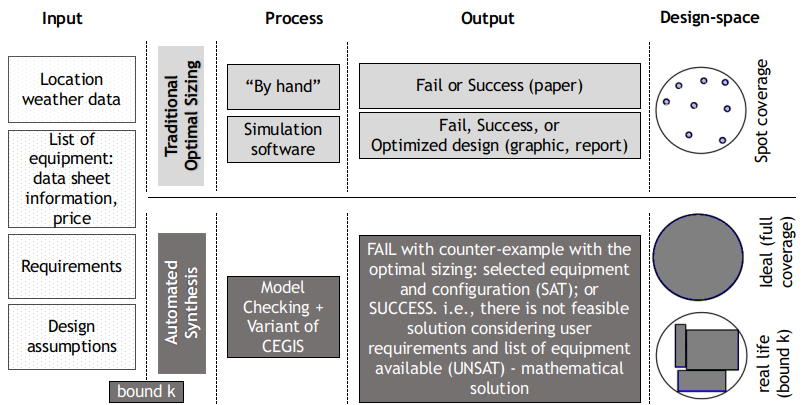
\includegraphics[width=1.0\textwidth]{optimalsizingprocess2g}
\centering
\caption{Comparison of optimal sizing methods}
\label{fig:optimization}
\end{figure}
 
\subsection{A Variant of CEGIS} 

Figure~\ref{CEGISalt} illustrates a variant of CEGIS, previously presented in Section ~\ref{sec:ProgramSynthesis}, Fig.~\ref{Counter-Example-Guided-Inductive-Synthesis}. This variant was created during the research for this thesis and will be detailed in this Section.

\begin{figure}[h]
	\centering
	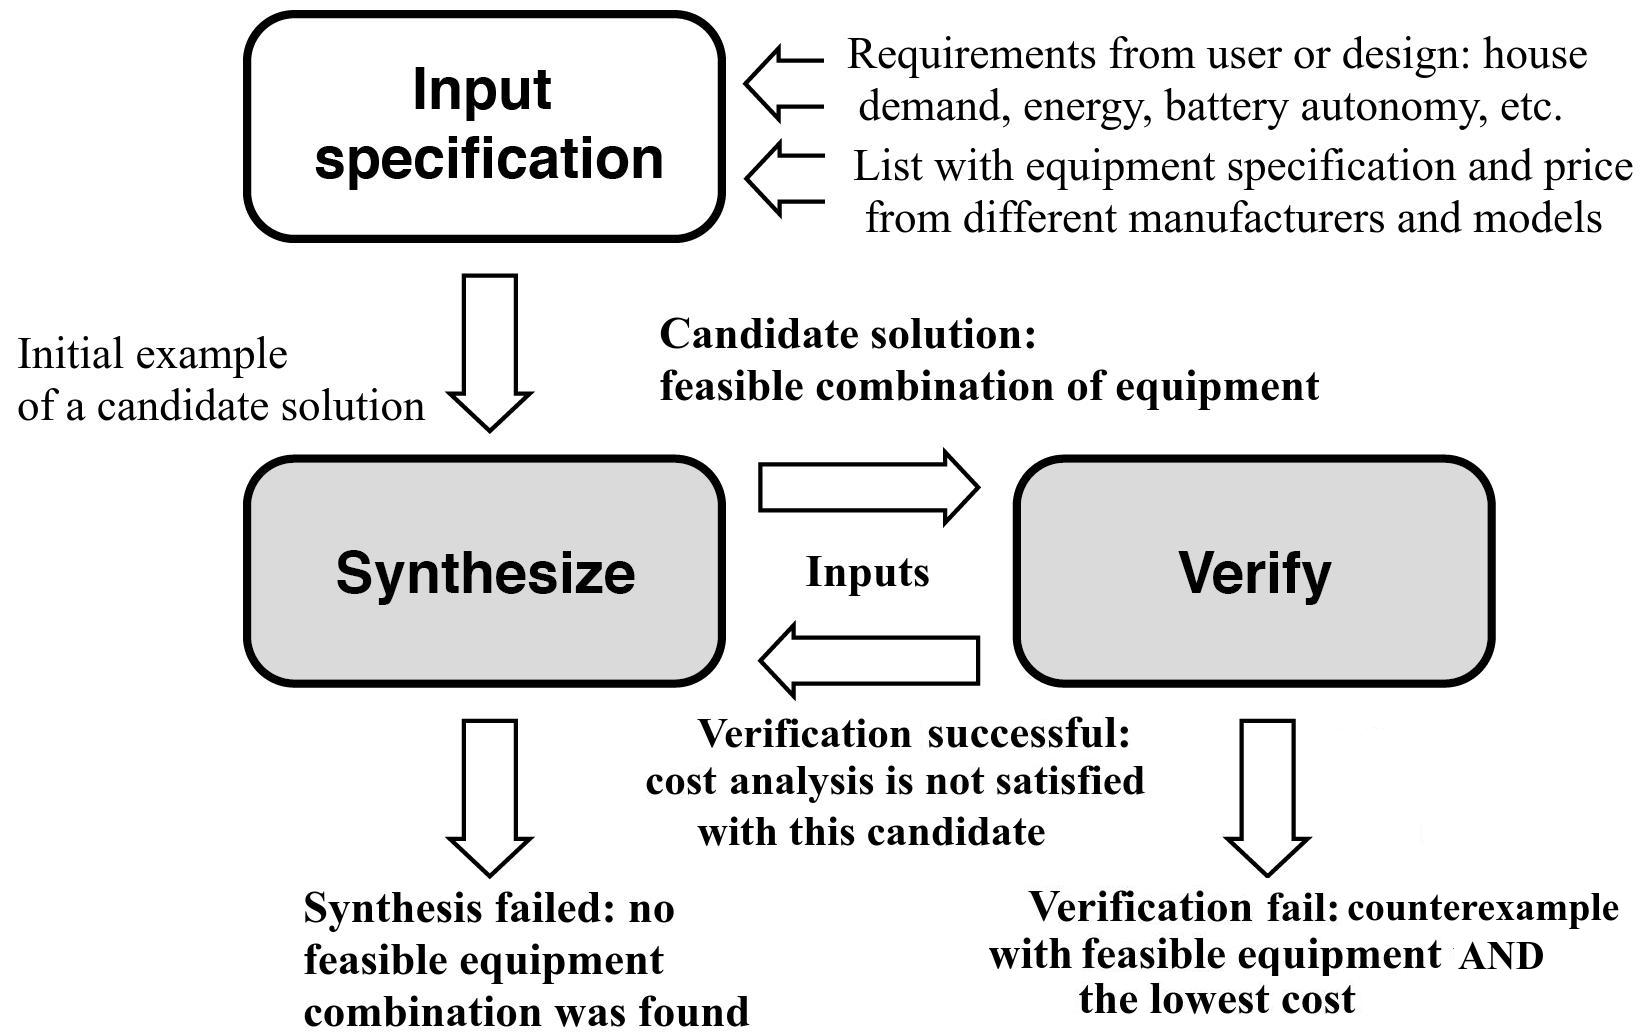
\includegraphics[width=0.75\columnwidth]{fig2_rev2.jpg}
	\caption{CEGIS applied to PV system sizing.}
	\label{CEGISalt}
\end{figure}

Examples of specification used by the proposed method include solar insolation (site dependent), house power demand, house  energy consumption, estimated load curve, AC voltage, and battery autonomy; we also provide a list of equipment specifications and prices from different manufacturers and models. Design assumptions are considered additional project specifications. The assumptions underlying optimal sizing are listed in Section~\ref{sec:OptAssumptions}.

The variant CEGIS used in the proposed approach differs in four specific aspects from the traditional CEGIS described in Figure ~\ref{Counter-Example-Guided-Inductive-Synthesis}: 

\begin{itemize}
\item There is no test vector and every candidate is generated during the run-time in the {\sc Synthesize} phase and sent to the {\sc Verify} phase; 
\item If the {\sc Verify} phase is unsuccessful, a new candidate is generated by {\sc Synthesize} 
\item The lower bound of the {\sc Verify} phase is incremented to search for the lowest cost; 
\item As a result, there is no refinement from the {\sc Verify} phase back to the {\sc Synthesize} phase, i.e. a new counterexample is not added to the {\sc input} set since a failure during the {\sc Verify} phase will only discard a given candidate that could be viable in the next iteration with a new lower bound.
\end{itemize}

Program synthesis engines that implement the CEGIS approach~\cite{sketch} can automatically produce solutions for a large variety of specifications; here we have used symbolic software verifiers based on SMT solvers.

Algorithm~\ref{alg:opt-algorithm} describes our pseudo-code to synthesize stand-alone PV systems using symbolic model checking. The analytical method of optimization was adopted, with LCC economic analysis and power reliability based on critical period criteria.

 \begin{algorithm}
 \caption{Synthesis algorithm}
 \begin{algorithmic}[1]
 \renewcommand{\algorithmicrequire}{\textbf{Input:}}
 \renewcommand{\algorithmicensure}{\textbf{Output:}}
  \REQUIRE weather data (temperature, solar irradiance), list of equipment (data sheet and price information), design requirements (load curve, peak demand, output voltage, battery autonomy), design assumptions (battery state of charge, criteria and objectives for technical and cost analysis)
 \ENSURE FAIL with counterexample showing the optimal sizing; SUCCESS, saying that the project has no feasible solution considering the requirements and the list of equipment available
  \STATE Initialize variables \\
  \STATE Declare list of PV panels, controllers, batteries, and inverters data and cost \\
%  \STATE Declare list of controllers data and cost \\
%  \STATE Declare list of batteries data and cost \\
%  \STATE Declare list of inverters data and cost \\
  \STATE Declare the maximum possible cost $MaxCost$  \\
  \STATE Declare power demand, power peak, energy consumption \\
  \STATE Declare battery autonomy, depth of discharge, AC voltage \\
  \FOR {$HintCost=0$ to $MaxCost$}
 	\STATE Declare non-deterministic variable to select PV Panel from list \\
 	\STATE Declare non-deterministic variable to select Controller from list \\
 	\STATE Declare non-deterministic variable to select Battery from list \\
 	\STATE Declare non-deterministic variable to select Inverter from list \\ 	
 	\STATE Calculate $E_{corrected}, \, E_{p} $ \\
	\STATE Calculate $N_{TPmin}, \, N_{PSmin}, N_{PPmin} $ \\
 	\STATE Calculate $C_{bank}$ \\
	\STATE Calculate $N_{BS}min, \, N_{BP}min, \, N_{B}total$ \\
	\STATE Requirement enforced by \textbf{assume}$(V_{c})$ \\
 	\STATE Calculate $I_{sc,amb}$ \\
 	\STATE Calculate $I_{c,min}$ \\
 	\STATE Requirement enforced by \textbf{assume}$(I_{c} \wedge V_{in}DC \wedge V_{out}AC)$ \\
%	\STATE Requirement enforced by \textbf{assume}$(V_{in}DC \wedge V_{out}AC )$ \\
%	\STATE Requirement enforced by \textbf{assume}$(V_{out}AC)$ \\
	\STATE Requirement enforced by \textbf{assume}$(Demand \wedge P_{surge})$ \\
%	\STATE Requirement enforced by \textbf{assume}$(P_{surge})$ \\
	\STATE non-deterministic variables hold feasible equipment and cost  \\
	\STATE $F_{obj} \leftarrow  N_{TP}*Panel_{Cost} \, + \, N_{TB}*Battery_{Cost} \, + Controller_{Cost} \, + \, Inverter_{Cost} \, + \, Installation_{Cost} \, + \, batrep_{Cost} \, + \, PWO\&M_{Cost}$ \\
	\STATE Violation check with \textbf{assert}$(F_{obj} > HintCost)$ \\
  \ENDFOR
 \RETURN $(\,)$ 
 \end{algorithmic} 
 \label{alg:opt-algorithm}
 \end{algorithm}

Our synthesis algorithm will synthesize constant values; 
it starts with the input of the manufacturer's data and prices of PV panels, batteries, charge controllers and inverters (line $2$). After that, we define user requirements, i.e. house requirements and design definitions, from lines $4$ and $5$. 

The \textit{for}-loop started at line $6$ controls the lowest cost of the PV solution. In particular, it starts with cost $0$ and stops only when the algorithm finds a feasible solution in which the cost breaks the $assertion$ stated in line $22$; if that happens, then our algorithm has found an optimal solution, thereby stating that the {\sc Verify} phase reached a satisfiable condition (\textit{SAT}). The $MaxCost$ value at line $6$ is just a very high value inserted as a limit to the \textit{for}-loop, that will never be reached because the optimal solution will be found first.

Our synthesis algorithm uses non-deterministic variables to choose one specific constant from a given list of PV panels, controllers, batteries and inverters (lines $7$ to $10$). This procedure ensures that our synthesis engine checks all combinations of items from each equipment, and combines them to assemble a viable (candidate) PV solution, which meets user requirements.

Next, we use Eq.~\eqref{eq:Ecorrected}, Eq.~\eqref{eq:Ep}, Eq.~\eqref{eq:NTPmin}, Eq.~\eqref{eq:NPSmin}, Eq.~\eqref{eq:NPPmin}, Eq.~\eqref{eq:Cbank}, Eq.~\eqref{eq:Nbtotal}, Eq.~\eqref{eq:iscamb} and Eq.~\eqref{eq:icmin} to calculate the sizing variables (lines $11$ to $17$). The directive \textit{assume} (lines $15$, $18$ and $19$) 
ensures compatibility of the items chosen from the list of equipment: the {\sc Verify} phase uses only items (among all the possible ones) that satisfy the statements of Lines $15$, $18$ and $19$. Line $15$ is specific to the charge controller voltage check. Line $18$ checks the inverter check $I_{c}$, the charge controller DC input voltage $V_{in}DC$, and charge controller AC output voltage $V_{in}DC$ check. Line $19$ ensures the power demand and the surge power of the inverter.
Therefore, our synthesis algorithm reaches line $20$ with one feasible solution, and the cost of that solution is calculated in $F_{obj}$ (line $21$). This cost is the equivalent to ~\ref{eq:LCC}, as described in Section ~\ref{sec:optcriteria}.

If our algorithm does not find a feasible solution among the item of equipment that were provided for our {\sc Synthesize} phase,  then the result is unsatisfiable (\textit{UNSAT}), i.e. the program finishes without finding a solution, indicating that it was not possible to combine the specific items of equipment in order to create a feasible solution. 

The main challenge for the {\sc Synthesize} phase is to find a feasible candidate solution for the constraints and user requirements. The challenge for the {\sc Verify} phase is to find the lowest acquisition cost from a list of equipment and components provided by the {\sc Synthesize} phase. 

Note that the process described here is completely automated and that a validation is performed by our {\sc Verify} phase to ensure that the approach is sound.

\subsection{Optimization Premises and Assumptions}
\label{sec:OptAssumptions}
%%%%%%%%%%%%%%%%%%%%%%%%%%%%%%%

This section contains premises and assumptions underlying the optimal sizing method, in relation to automated synthesis and simulation software.

In line $2$ of Algorithm~\ref{alg:opt-algorithm}, the synthesis engine is provided with a list of forty items of equipment from ten different manufacturers in order to allow the engine to choose from among all items of PV sizing. The necessary technical information was collected from data sheet of each item. In addition, the price of each item was obtained from available market quotation, in US dollars. All the other currencies were converted to US dollars equivalents at the exchange rate of the day.

With respect to power reliability, the critical period solar energy method will be used~\cite{Pinho}, as described in Section~\ref{sec:sizing}. The usual way is to use loss of load probability (LOLP) or loss of power supply probability (LPSP). However, due to the fact that in this study we are considering neither site characteristics nor load changes over time, which demand historical data, the reliability analysis will be developed only by the critical period method of PV sizing.

Financial analysis details:
\begin{itemize}
	\item LCC lifetime considered: $20$ years;
	\item Installation costs: these include delivery to the isolated community and the actual installation costs: $5$\% of total cost~\cite{Agrener2013};
	\item Value of the discount rate or interest rate: $10$\%, a good rate, considering financial investments in developing countries;
	\item Annual operation and maintenance costs: based on past PV projects of similar size in the Brazilian Amazon, the sum of US\$ 289.64~\cite{Agrener2013} will be adopted. This cost includes battery replacement based on a lifetime of $4$ years for lead-acid batteries, plus inverters and controller replacement (every $10$ years). This means that there will be three battery bank and one inverter-controller replacement during the LCC analysis.
\end{itemize}

The PV system optimization technique adopted here is the intuitive method, since the average daily value of solar irradiance is used in the mathematical model, without considering battery state of charge, or even the random nature of solar irradiation and meteorological conditions. Therefore, all the computational effort will be concentrated on our automated synthesis algorithm.

With regard to batteries, the voltage of the system (DC bus) is set at $24$ V DC (but this can be adjusted to $12$ or $48$ V in the code).

HOMER Pro details:

\begin{itemize}
	\item HOMER Pro does not provide for the LCC cost in its reports. However, it has NPC and LCOE. For this reason, NPC was used to obtain LCC in order to allow the comparison among tools;
	\item The optimization analysis of HOMER Pro permits the definition of a load curve and temperature on the basis of data collected automatically from online databases. However, in order to enable a correct comparison, the curve load and the temperature were defined exactly the same as automated synthesis tools;
	\item Battery autonomy is not a parameter that the user can set when using HOMER Pro. The tool will always meet the user requirement, i.e. the load curve, $365$ days a year;
	\item HOMER Pro does not have an item of equipment explicitly labeled charge controller. It uses a controller resource that can perform in two different ways, depending on optimization choice or user choice: load following or cycle charging~\cite{HOMER}. During the tests  'load following' controller was chosen: it produces only enough power to meet the demand~\cite{HOMER};
	\item A 5\% of capacity shortage was assumed, equivalent to 95\%  availability of the PV system. By definition, availability is the percentage of time during which a power system is capable of meeting the load requirements~\cite{Khatib2014}. For critical loads, 99\% is considered acceptable, while in an ordinary residential electrical load, 95\% is considered acceptable;
	\item A string of two batteries was assumed in order to match the system voltage of $24$ V DC used by the automated synthesis tool;
	\item The premise adopted when using HOMER Pro was that the user does not know the optimal solution, and that in order to obtain this solution it is necessary to include (at the design phase of the tool) generic PV and battery modules that HOMER Pro will search for the optimized power of each component. With that in mind, a generic flat plate PV of $1$ kW was included and generic lead-acid batteries of $1$ kW also (and with capacity of $83.4$ Ah in accordance with HOMER Pro modeling). HOMER, during run-time, decides the size in kW of each module, based on feasibility and lower cost.	
\end{itemize}

\section{General Assumptions}

The general assumptions for the scientific method of automated synthesis are the same presented in Section~\ref{sec:assumptions}, with respect to the code in ANSI-C, to the bound $k$, to the simulation tool comparison, and to the battery state of charge.

%---------------------------------------------------------------------------
\section{Description of the Case Studies} 
%---------------------------------------------------------------------------

The proposed synthesis approach was evaluated in  seven stand-alone PV system case studies: 

\begin{itemize}
\item Case Study 1: Power peak: 342 W, power surge: 342 W, energy consumption: 3,900 Wh/day, battery autonomy: 48 h;
\item Case Study 2: Power peak: 814 W, power surge: 980 W, energy consumption: 4,880 Wh/day, battery autonomy: 48 h;
\item Case Study 3: Power peak: 815 W, power surge: 980 W, energy consumption: 4,880 Wh/day, battery autonomy: 12 h;
\item Case Study 4: Power peak: 253 W, power surge: 722 W, energy consumption: 3,600 Wh/day, battery autonomy: 48 h;
\item Case Study 5: Power peak: 263 W, power surge: 732 W, energy consumption: 2,500 Wh/day, battery autonomy: 48 h;
\item Case Study 6: Power peak: 322 W, power surge: 896 W, energy consumption: 4,300 Wh/day, battery autonomy: 48 h;
\item Case Study 7: Power peak: 1,586 W, power surge: 2,900 W, energy consumtion: 14,000 Wh/day, battery autonomy: 48h.
\end{itemize}

These case studies were defined based on the usual electrical load found in riverside communities in the State of Amazonas,  Brazil~\cite{TrindadeCordeiro19, Agrener2013}, with the exception of case 7, that was idealized as a small town solution to support a few lamps and a 12 kBTUs air-conditioner.

%---------------------------------------------------------------------------
\section{Objectives and Setup}
\label{sec:synthesissetup} 
%---------------------------------------------------------------------------

The evaluation aims to answer two experimental questions: 

\begin{enumerate}

\item[EQ1] \textbf{(soundness)} does the proposed automated synthesis approach provide correct results?

\item[EQ2] \textbf{(performance)} how do the software verifiers compare to each other?

\end{enumerate}

All experiments regarding the verification tools were conducted 
on an otherwise idle Intel Xeon CPU E5-4617 ($8$-cores) with 
$2.90$ GHz and $64$ GB RAM, running Ubuntu $16.04$ LTS $64$-bits. 
For HOMER Pro, an Intel Core i5-$4210$ ($4$-cores) was used, 
with $1.7$ GHz and $4$ GB RAM, running Windows 10. 
The experiments were conducted with a predefined time-out of $240$ minutes.

Three start-of-the-art verification tools, CBMC\footnote{Command-line: \$ cbmc -\phantom{}-unwind 100 filename.c -\phantom{}-trace} version 5.11 with MiniSat 2.2.1~\cite{Kroening}, ESBMC\footnote{Command-line: \$ esbmc filename.c -\phantom{}-no-bounds-check -\phantom{}-no-pointer-check -\phantom{}-unwind 100 -\phantom{}-boolector} version 6.0.0 with the  Boolector 3.0.1 solver~\cite{Brummayer}, %UAutomizer\footnote{Command-line: \$ ./Ultimate -tc config/AutomizerReach.xml -s config/svcomp-Reach-32bit-Automizer\_Default.epf -i filename.c -\phantom{}-traceabstraction.limit.analysis.time 900 -\phantom{}-traceabstraction.stop.after.first.violation.was.found false -\phantom{}-cacsl2boogietranslator.overapproximate.operations.on.floating.types false -\phantom{}- cacsl2boogietranslator.assume.nondeterminstic.values.are.in.range false -\phantom{}-rcfgbuilder.add.additional.assume.for.each.assert true -\phantom{}-rcfgbuilder.simplify.code.blocks true -\phantom{}-rcfgbuilder.size.of.a.code.block LoopFreeBlock}, 
and CPAchecker\footnote{Command-line: \$ scripts/cpa.sh -heap 64000m -config config/bmc-incremental.properties -spec config/specification/sv-comp-reachability.spc filename.c} version 1.8 with MathSAT 5.5.3~\cite{mathsat5}, were used as verification engines to compare the proposed approach effectiveness and efficiency. Note that ``incremental'' ESBMC with the SMT solver Z3 version 4.7.1~\cite{DeMoura} was tried\footnote{Command-line: \$ esbmc filename.c -\phantom{}-no-bounds-check -\phantom{}-no-pointer-check -\phantom{}-unwind 100 -\phantom{}-smt-during-symex -\phantom{}-smt-symex-guard -\phantom{}-z3} as an alternative to use less computing memory. The Simulation tool HOMER Pro version $3.13.1$ was used for comparative purposes.

%---------------------------------------------------------------------------
\section{Experimental Results}  
\label{sec:synthesisresults}
%---------------------------------------------------------------------------

The results are presented at Table~\ref{tab1}. 

\begin{table}
\caption{Case studies and results: optimization of stand-alone PV systems.}\label{tab1}
\begin{scriptsize}
\begin{tabular}{|c|c|c|c|c|}
\hline
\hline
Tools & \makecell{CBMC 5.11 \\(MiniSat 2.2.1)}& \makecell{ESBMC 6.0.0 \\(Boolector 3.0.1 /\\Z3 4.7.1)}& \makecell{CPAchecker 1.8\\(MathSAT 5.5.3)}& HOMER Pro 3.13.1\\
\hline
\hline
Specification & Result & Result & Result & Result \\
\hline
\makecell{\textbf{Case Study 1}\\Peak:342W\\Surge:342W \\E:3,900Wh/day\\Autonomy:48h} & OM & TO / IF & \makecell{SAT (172.03 min) \\NTP:1$\times$340W (1S)\\NBT:8$\times$105Ah (2S-4P)\\Controller 15A/75V\\Inverter 700W/48V\\LCC: US\$ 7,790.53} & \makecell{(Time: 0.33 min)\\2.53 kW of PV\\NBT:12$\times$83.4Ah (2S-6P)\\0.351kW inverter\\LCC: US\$ 7,808.04}\\
\hline
\makecell{\textbf{Case Study 2}\\Peak:814W\\Surge:980W\\E:4,880Wh/day\\Autonomy:48h} & OM & TO / IF & \makecell {SAT (228.7 min) \\NTP:2$\times$330W (2S)\\NBT:10$\times$105Ah (2S-5P)\\Controller 20A/100V DC\\Inverter 1,200W/24V \\LCC: US\$ 8,335.90} & \makecell{(Time: 0.18 min)\\3.71 kW of PV\\NBT:20$\times$83.4Ah (2S-10P)\\0.817kW inverter\\LCC: US\$ 12,861.75} \\
\hline
\makecell{\textbf{Case Study 3}\\Peak:815W\\Surge:980W\\E:4,880Wh/day\\Autonomy:12h} & OM & TO / IF & \makecell {SAT (166.13 min) \\NTP:4$\times$150W (4S)\\NBT:4$\times$80Ah (2S-2P)\\Controller 15A/100V DC\\Inverter 1,200W/24V \\LCC: US\$ 7,306.27} & Not possible \\
\hline
\makecell{\textbf{Case Study 4}\\Peak:253W\\Surge:722W\\E:3,600Wh/day\\Autonomy:48h} & OM & TO / IF & \makecell {SAT (143.71 min) \\NTP:4$\times$150W (4S)\\NBT:10$\times$80Ah (2S-5P)\\Controller 15A/75V\\Inverter 750W/24V \\LCC: US\$ 7,816.31} & \makecell{(Time: 0.23 min)\\2.42 kW of PV\\NBT:12$\times$83.4Ah (2S-6P)\\0.254kW inverter\\LCC: US\$ 7,677.95}\\
\hline
\makecell{\textbf{Case Study 5}\\Peak:263W\\Surge:732W\\E:2,500Wh/day\\Autonomy:48h} & OM & TO / IF & \makecell {SAT (134.93 min) \\NTP:1$\times$340W (1S)\\NBT:6$\times$105Ah (2S-3P)\\Controller 15A/75V\\Inverter 400W/24V \\LCC: US\$ 7,252.14} & \makecell{(Time: 0.18 min)\\1.59 kW of PV\\NBT:10$\times$83.4Ah (2S-5P)\\0.268kW inverter\\LCC: US\$ 6,175.57} \\
\hline
\makecell{\textbf{Case Study 6}\\Peak:322W\\Surge:896W\\E:4,300Wh/day\\Autonomy:48h} & OM & TO / IF & \makecell {SAT (235.75 min) \\NTP:2$\times$200W (2S)\\NBT:10$\times$105Ah (2S-5P)\\Controller 15A/75V\\Inverter 400W/24V \\LCC: US\$ 8,287.23} & \makecell{(Time: 0.22 min)\\3.15 kW of PV\\NBT:14$\times$83.4Ah (2S-7P)\\0.328kW inverter\\LCC: US\$ 9,112.45} \\
\hline
\makecell{\textbf{Case Study 7}\\Peak:1,586W\\Surge:2,900W\\E:14,000Wh/day\\Autonomy:48h} & OM & TO / IF & TO & \makecell{(Time: 0.20 min)\\12.5 kW of PV\\NBT:66$\times$83.4Ah (2S-33P)\\1.60kW inverter\\LCC: US\$ 41,878.11} \\
\hline
\hline
\end{tabular}
\\Legend: OM = out of memory; TO = time out; IF = internal failure, E = energy.
\end{scriptsize}
\end{table}

CPAchecker was able to synthesize optimal sizing in six 
out of the seven case studies (cases $1$ - $6$): the result was produced within the time limit, which varied from $134.71$ to $235.75$ minutes. Fig.~\ref{fig:CPAoptc1} illustrates the result of case 4 with the optimal sizing appearing on the left size as the integer $8$ for the solar panel (which is the model RSM36-6-150P from the manufacturer Risen), battery $0$ refers to the model 12MF80 of 80 Ah from Moura, charge controller $1$ refers to the model 15A-75V MPPT from Victron  Energy, and the inverter number $3$ refers to the model IP350-11 from Epever (750 W). The variables NTP, NPS, NPP, NPS, NBP, and NBTotal, also presented in the counterexample as well, shows the number of panels and batteries and how they are connected.

Only case study $7$ led to a \textit{time out} result in CPAchecker, i.e.  it was not solved within $240$ minutes. This is illustrated in Fig.~\ref{fig:cpaoptcase7}. However, this CPAchecker time-out limitation is removed, the verifier is able to solve the optimization in $44.97$ hours. The violation (SAT result) indicated in Table~\ref{tab1} 
is the $assert$ of line $22$ from Algorithm~\ref{alg:verification-algorithm}. %The results were tested by manual PV sizing and were sound (\textit{RQ1}). %, linking a feasible technical solution with the lowest cost possible, considering the equipment that were inputted to the code. 

\begin{figure}[h]
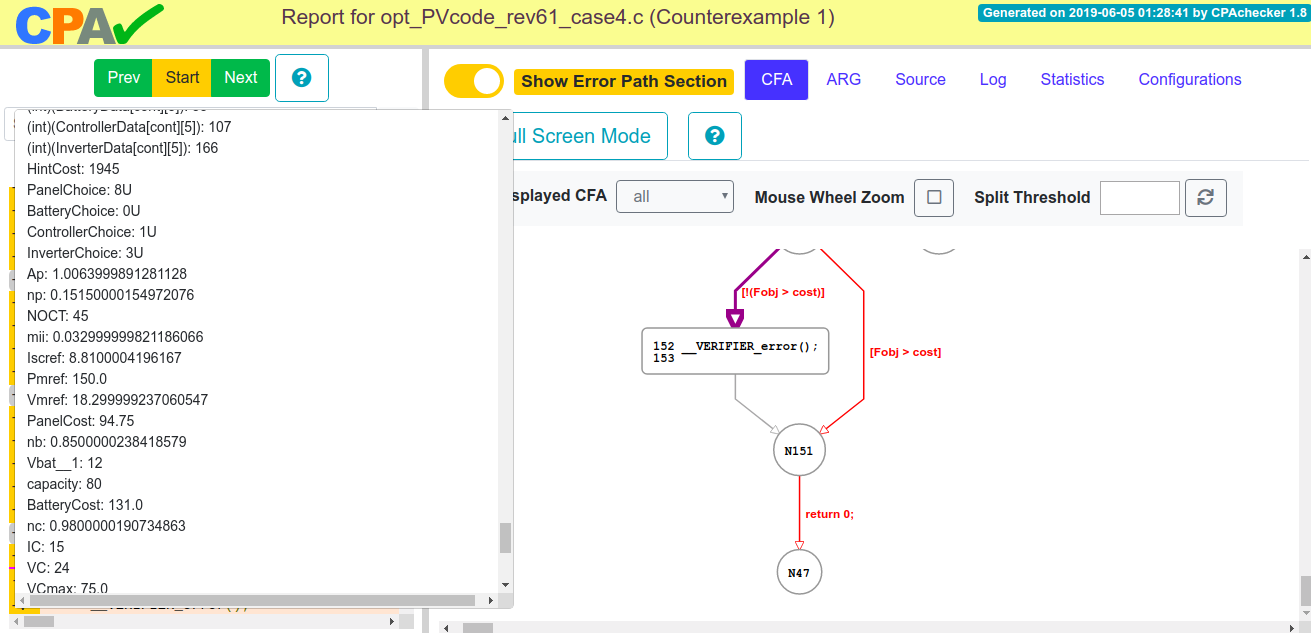
\includegraphics[width=1.0\textwidth]{CPA_opt_c4.png}
\centering
\caption{Counterexample generated by CPAchecker after validation of case 4 (file Counterexample.html).}
\label{fig:CPAoptc1}
\end{figure}

\begin{figure}[h]
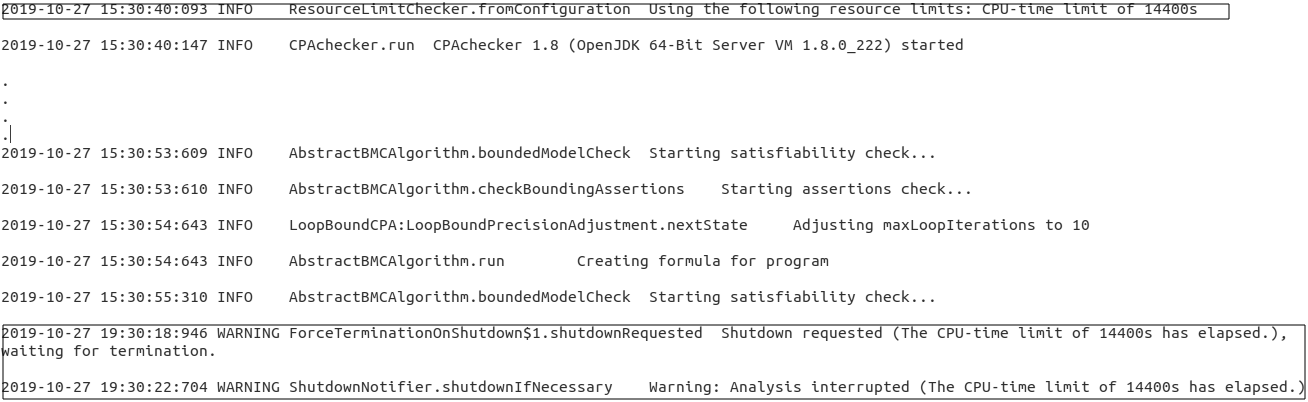
\includegraphics[width=1.0\textwidth]{CPAchecker_timeout_case7.png}
\centering
\caption{CPAchecker time out result for case 7 optimization (file CPALog.txt).}
\label{fig:cpaoptcase7}
\end{figure}

CBMC and ESBMC are unable to produce any conclusive result. \textit{Internal failure}, \textit{time out}, or \textit{out of memory} situations occurred; this partially answers the \textit{EQ2}. Note that the internal failure presented by ESBMC was a Z3 solver issue (a bug), which will require an updated version of ESBMC to fix. Similar to CPAchecker, if the \textit{time out} is removed from ESBMC with the SMT solver Boolector, then the verifier is able to obtain the automated synthesis in $73.18$ hours for case study $2$. CBMC, on the other hand,  could present some result only if the RAM memory of the system was expanded in order to avoid the out of memory issue.

HOMER Pro was able to evaluate six case studies (cases $1$, $2$, $4$, $5$, $6$, and $7$), and in under $30$ seconds, much faster than the proposed automated synthesis tool (cf.~\textit{EQ2}). Case study $3$ could not be simulated since HOMER Pro does not have the battery autonomy adjustment feature, i.e. the tool always tries to feed the given load with electricity $365$ days/year. 

Fig.~\ref{fig:homeroptc4} illustrates parts of the 9-page PDF report presented by HOMER Pro, specifically for case 4.

\begin{figure}[h]
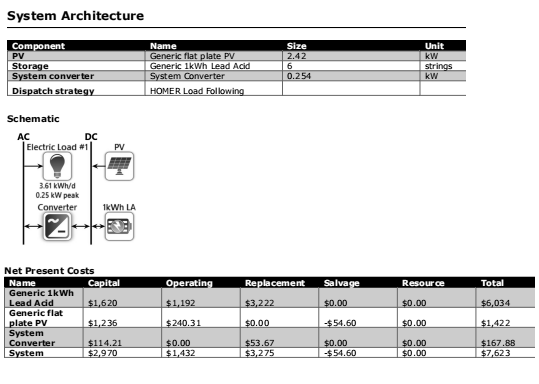
\includegraphics[width=0.8\textwidth]{homeroptc4.png}
\centering
\caption{Optimization report (partial) from HOMER Pro (case 4).}
\label{fig:homeroptc4}
\end{figure}

Certain other HOMER Pro drawbacks were also noted:

\begin{itemize}
\item System equipment does not include an explicit charge controller . HOMER Pro includes a controller automatically just to simulate the charge/discharge of batteries and to meet the load requirement; however, without costs or even with electrical characteristics such as maximum current and voltage, which are common during PV sizing;
\item HOMER Pro requires the inclusion of some battery specification to initiate optimization; however, it does not change the electrical specifications during simulation; the results presented are multiples of the original battery type suggested by the user. For example, it was started with a $83.4$ Ah lead-acid battery and during simulation, HOMER Pro did not try to use other capacities or types;
\item HOMER Pro does not present the optimal solution in terms of connections of PV panel arrays, just the total in terms of power, i.e. it presents neither the models and the power of each PV panel nor the total of panels in series or parallel.
\end{itemize}

%%%%%%%%%%%%%%%%%%%%%%%%%%%%%%%%%%%%%%%%%%%%%%%%%%%%%%%%%%%%%%%%%%%%
\subsection{Comparison Between Formal Synthesis and HOMER Pro}
%%%%%%%%%%%%%%%%%%%%%%%%%%%%%%%%%%%%%%%%%%%%%%%%%%%%%%%%%%%%%%%%%%%%

Comparing the results of the formal synthesis against those of CPAchecker and HOMER Pro, it was observed that most results are quite similar, 
in terms of technical solution and cost (cf. Table~\ref{tab1}). 

Particularly in the case of LCC, the cost was very close in cases $1$, $4$, $5$ and $6$, with differences varying from $0.23$\% to $17.4$\%. Even adopting the same price per kW for PV panels, inverters, and batteries, HOMER Pro does not use costs related to charge controllers, which were introduced into the CPAchecker modeling. The premise used in CPAchecker to adopt a fixed annual cost for operation and maintenance can produce some impact as well on this discrepancy; however, it is not significant since the annual cost is too small when compared to the resulting LCC value.

However, there exists a huge divergence in case study $2$, where the costs presented by HOMER Pro were $54$\% higher than the automated synthesis tool, probably because the operation and maintenance costs assumed by the automated synthesis tool were underestimated for that specific load. 

In general, the PV panels and battery bank were larger in HOMER Pro than with the formal synthesis approach, and that discrepancy is not easy to address without some real systems validation. The mathematical models are different and particular parameters can be tuned as well in each approach, and that can justify the difference, which was presented in all the case studies. As a comparison, consider case study $1$: the optimal solution provided by HOMER Pro requires $7$ $times$ more PV panels than the solution presented by the synthesis tool, and HOMER Pro does not show the arrangement of arrays (i.e. the number of series and parallel PV panels); the battery bank presented by HOMER Pro provides a capacity of $500.4$ Ah ($6 \times 83.4$), while the synthesis tool presented an optimal solution with a total capacity of $420$ Ah ($4 \times 105$). 

Comparing the optimization results with those the real-world, the author had four PV systems deployed and monitored since June $2018$ in a riverside community in State pf Amazonas, Brazil, with demands  similar to those of case studies $1$, $4$, $5$, and $6$, always with a $3$ $\times$ $325$ W ($3$S) panels and $4$ $\times$ $220$ Ah ($2$S-$2$P $= 440$ Ah) lead-acid batteries. These solutions are closer to the result presented by the proposed formal synthesis approach than that of HOMER Pro, thereby showing that the solution is sound, which answers \textit{EQ1}.

HOMER Pro suggests a value in kW for the inverters that is very close to the peak of every case study, and it is just a reference value and not a commercial value of the inverter employed. The proposed synthesis tool, however, presents inverters that are commercial and can be bought off-the-shelf. This is a clear advantage of the formal synthesis method.

As was reported in section~\ref{sec:synthesisresults}, HOMER Pro does not include charge controllers as an explicit item of equipment in its mathematical model; only the synthesis tool presents a commercial controller and includes it during the cost analysis. The formal synthesis method, therefore, presents more reliable results than HOMER Pro.

Case study $7$ was not solved by the synthesis tool within the time limit established during the experimental phase. Case study $3$ could not be simulated in HOMER Pro, because of its restriction on setting battery autonomy, thus leaving both without parameters to compare.

Summarizing, the synthesis tool is capable of presenting a solution which is far more detailed and closer to commercial conditions than the solution presented by HOMER Pro. In particular, the automated synthesis method can provide all the details of every component of a PV system solution, with complete electrical details from the manufacturer data sheet, including  the model of the component, nominal current and voltage. In this respect, even the name of the manufacturer can be cited (in Table~\ref{tab1} it was removed to avoid unauthorized advertising).
%used with the SMT incremental mode\footnote{Command-line: \$ esbmc filename.c -\phantom{}-no-bounds-check -\phantom{}-no-pointer-check -\phantom{}-unwind 100 -\phantom{}-smt-during-symex -\phantom{}-smt-symex-guard -\phantom{}-z3} enabled with the goal of reducing memory usage; we have also used the SMT solver Z3 version 4.7.1~\cite{DeMoura}.

%%%%%%%%%%%%%%%%%%%%%%%%%%%%%%%%%%%%%%%%%%
\section{Threats to validity}
%%%%%%%%%%%%%%%%%%%%%%%%%%%%%%%%%%%%%%%%%%

In this Section, a favorable assessment was made of the proposed formal synthesis method. Nevertheless, three threats to the validity of the experimental results were also identified, which can be further assessed and 
constitute future work: 

\begin{itemize}
\item ($1$) improvement to the power reliability analysis: inclusion of loss of load probability or loss of power supply probability, in order to increase the accuracy of the analysis; 
\item ($2$) the cost analysis is well tailored to Brazilian Amazon; however, a broad analysis of other isolated areas must be  performed in order to make the optimization general in terms of applicability; 
\item ($3$) deployment in the field of PV systems sized using the synthesized results in order to validate them.
\end{itemize}


\section{Conclusion}

In this Chapter we showed in detail how the state-of-the-art computer science method of automated synthesis has been adapted to use in stand-alone solar PV systems in order to obtain optimal project sizing. Moreover, it was possible to illustrate how the proposed method compares with the traditional use of a simulation tool for the same purpose.

Detailed diagrams, flowcharts and algorithms with pseudo-code were presented as support for the proposed work and to aid understanding. Also listed, were the assumptions underlying the automated verification and simulation software. 

Comparison of verifiers with the proposed automated synthesis using model checking was made, in order to obtain the optimal sizing of stand-alone solar PV systems, which showed that CPAchecker had the best overall performance. CBMC and ESBMC were not conclusive for all the cases, reaching the \textit{time out} stipulated ($240$ minutes) or being \textit{out of memory}. CPAchecker was unable to present a conclusive result only in case $7$ (\textit{time out}).

A comparison with a specialized simulation tool was also made, however only $5$ case studies (case $1$, case $2$, case $4$, case $5$, and case $6$) compared to the presented result. Some limitations of the simulation tool, mainly related to not allowing battery autonomy setup, and the $time-out$ or $out of memory$ messages presented by the verifiers, restricted the comparison between the automated verification tools and the simulation tools. However, when the comparison was possible, it was noticeable that the LCC came very close, and that HOMER Pro overestimated the sizing.

Based on the fact that mostly case studies were deployed in the field (case $1$, case $4$, case $5$, and case $6$), with regular visits to conduct interviews with the residents, and consult the monitoring system in those houses, it was possible to compare the computer assisted results with the real-world employment of stand-alone solar PV systems. The final conclusion was that the proposed tool is sound, with an acceptable performance, and a higher quality output.

\chapter{Conclusions}
\label{chap:conclusions}
\fancyfoot[CO,CE]{Conclusions}
At this final chapter, we present the conclusions about the research done and the results obtained during the Doctoral process, including the two scientific methods or techniques from computer science that were applied to solar PV systems. Moreover, a list of future contributions, which probably will foster the creation of a research group that applies model checking to electrical systems (not only renewable sources) closes the work.

\section{Main Contributions}

Our contributions can be split in two, each one concerning the scientific methods proposed with the use of model checking to solar PV systems, and the tools created to validate it.

Related to the first contributions, depicted with details in ~\autoref{chap:automatedverification}, it was described and evaluated an automated verification method to validate over the time a given stand-alone PV system design, and see if it meets its user and electrical requirements using software model checking techniques. There are a lot of possibilities to perform that validation, as testing, laboratory measuring, or even simulation (used before field deployment, as our proposal); however, we showed, supported by an algorithm that uses our approach, moreover supported by case studies, by monitoring data from field, and from interview if the owners, that our approach is feasible and effective.

It was considered five case studies from real PV systems deployed in five different sites, ranging from $700$ W to $1,200$ W (inverter specification); and three state-of-art verification engines were considered (ESBMC, CBMC, and CPAchecker). Although the verification method that we proposed takes longer than simulation methods, it is able to avoid the battery bank oversize produced by the simulation tool in houses $1$, $2$, $3$, and $4$. This result was validated by the sized systems deployed at the field.

Moreover, it was not necessary to 'adapt' the tool, since the specialized simulation tool (HOMER Pro) had to be adjusted in order to not perform the optimization of the system. In addition, only the proposed method of automated verification was possible to validate a system with a specific battery autonomy, since HOMER Pro does not have this feature.

%In a nutshell, our proposed PV system validation method, who check the size of inputted PV system, and verifies it over the time, was feasible and effective, supported by a algorithm written to implement the method, by a comparative with a commercial simulation tool, and by real data collect at the field.
%
Related to the verification engines comparative, the ESBMC with the Z3 solver executed in the 'incremental SMT' configuration presented the better performance (around four times faster than CBMC), used less RAM memory (less than $2$ GB when compared to $9.2$ GB of CBMC and 19.2GB of CPAchecker), and all the results were sound because the PV owners and the monitoring system validated the possible flaws that the system could be presenting in the field.
%New tests must be performed, in an improved setup (i.e., better computing performance) with the goal of obtaining verification results in shorter times than the ones obtained in this study. 

Furthermore, we have also contributions from the method depicted in ~\autoref{chap:automatedsynthesis}. We have described and evaluated an automated synthesis method to obtain the optimal size of the PV system using software model checking techniques. The focus was on the synthesis method to obtain the optimal solution based on formal methods, which can cover better the design-space as opposed to simulation tools. Our thesis produced a methodological research with innovative value regarding the first use of automated synthesis for optimal sizing of solar PV systems.

We proposed a variant of CEGIS synthesis process, working with just one feasible solution from the {\sc Synthesize} phase, and a refinement from the iterative search from the {\sc Verify} phase, which allows the optimization of stand-alone PV systems with the best compromise between power reliability and system cost analysis. Our algorithm, that implements the method, uses a data base of commercial equipment from the marketing, including the price. In order to validate the method, it was considered seven case studies from PV systems in two different sites of the Amazonas State in Brazil, ranging from $253$\,W to $1,586$\,W peak; and three state-of-art verification engines were considered (ESBMC, CBMC, and CPAchecker), in addition to a specialized off-the-shelf simulation tool (HOMER Pro) in order to compare the results. In terms of performance and better results, CPAchecker was the winner and used for the comparative with the simulation tool. 

In summary, our synthesis proposal is capable of presenting a solution, which is far detailed and close to the commercial reality than the solution presented by HOMER Pro. In particular, our method can provide all the details of every component of a PV system solution, with complete electrical details from data sheet of manufacturers, including the model of the component, nominal current, and voltage; we also cover the charge controller, which is unavailable in HOMER Pro. Note that our automated synthesis tool took longer to find the optimal solution than HOMER Pro; however, the presented solution is sound and complete; it also provides a list of equipment to be bought from manufacturers. %Moreover, we extended the CEGIS synthesis method and implemented this extension within our proposed formal synthesis tool, which allows the optimization of stand-alone PV systems with the best compromise between power reliability and system cost analysis.


\section{Future Work Directions}

As the focus here was stand-alone solar PV systems, one future work will be also consider other types of renewable energy and even hybrid ones to allow the method to verify and to obtain the optimal sizing of typical rural electrification systems.

Related to automated sizing, the author plan to improve the power reliability analysis, 
to address the restriction to only allow automated synthesis of riverside communities in the Amazonas state (Brazil), and to validate some cases with deployed PV systems in isolated communities.

It is planned to develop the code of a general purpose simulation tool, using the same mathematical model employed for the model checking methods of this work, to include it in the comparative in order to cover all the possibilities to validate or optimize solar PV systems.

One future long term direction is to foster the creation of a research group in automated verification and synthesis applied to electrical systems; and a international network of researchers in model checking applied to electrical systems.


\section{Concluding Remarks}

The automated verification and automates synthesis methods demonstrate the effectiveness and the potential of use in stand-alone solar PV systems. Some issues must be addressed in order to improve the tools, as performance and the human-computer interaction, however the work has potential and it is promising.

About license and the use of tools that the author employed at this work, must be noticed that HOMER Pro is available only for Microsoft Windows and its annual standard subscription costs US\$ $504.00$~\cite{HOMER}; the verifiers, as CPAchecker, ESBMC and CBMC, and their solvers, they are  based on open source software license and usually allows the users to freely use, modify, and distribute licensed product. Permission is granted, free of charge, to use this software for evaluation and research purposes (and that is a advantage when compared to commercial tools); therefore, some of the licenses do not allow the software to be used in a commercial context.

Based on the fact that the tools detailed here have not similarity in past work in the world, can be concluded that it was produced original research that expands the boundaries of knowledge, putting cutting-edge computer science methodologies to solve typical electrical engineering problems and to improve the design of systems.

And last, but not least important to report, besides the fact that the goal of a PhD is to make a contribution to the body of human research, one of the great things about PhD is you will be able to conduct your own research. In that direction, we can say that with the technique proposed here (formal methods using automated verification and model checking) to energy sector, there is a vast field of future applications and developments, using different renewable sources, as biomass, as wind, or even hybrid, with different mathematical models and requirements; and including smart grids, or electrical systems in general. Few research has been made until now, and the scenario is auspicious from now on.



\appendix
\chapter{List of Publications}
\label{chap:publications}
\fancyfoot[CO,CE]{Appendix}
%\textbf{List of Publications}
%
Here there are a list of papers that were written during the Thesis elaboration and the status of every submission until the date of this document.

\section{Journals}

Trindade, A., Cordeiro, L. \textbf{Automated Formal Verification of Stand-alone Solar Photovoltaic Systems}, submitted: 8-May-2019 , status: in review (2nr round, since 16-July-2019) by Elsevier Solar Energy (Impact Factor 4.374, CAPES A1 Interdisciplinary, CAPES A1 Engineering IV ) \url{https://www.journals.elsevier.com/solar-energy}

Trindade, A., Cordeiro, L. \textbf{An automated formal synthesis optimization method for sizing of stand-alone solar photovoltaic systems: case studies and comparative}, submitted: 29-June-2019, resubmitted: 09-July-2019, status: under review by Elsevier Applied Solar (Impact Factor 7.9, CAPES A1 Interdisciplinary, CAPES A2 Engineering IV, CAPES B1 Computer Science) \url{https://www.journals.elsevier.com/applied-energy}


\section{Congress}

Trindade, A., Cordeiro, L. \textbf{Automated Formal Synthesis of Optimal Sizing for Stand-Alone Solar Photovoltaic Systems}, submitted: 06-MAY-2019, status: under review by The IEEE/ACM Automated Software Engineering (ASE 2019) Conference (New Ideas Papers) \url{https://2019.ase-conferences.org/track/ase-2019-papers}

\fancyfoot[CO,CE]{References}
%\printbibliography
\renewcommand\bibname{References}
%\bibliographystyle{abntex2-num}
\bibliography{trindadeThesis}{}


\end{document}
